%% GRB 081222 — timing and spectral analysis (single-pulse campaign, burst #2)
%% DRAFT — all numbers real and provisional-flagged; one section per pipeline step.
\documentclass[twocolumn]{aastex631}

\newcommand{\grb}{GRB~081222}
\newcommand{\trig}{bn081222204}
\newcommand{\pgstat}{\mathrm{PGstat}}

\shorttitle{\grb}
\shortauthors{Chand, Sharma, \& Joshi}

\begin{document}

\title{\grb}

\author{Agentic AI Report by Vikas Chand, Khushboo Sharma, and Jagdish C. Joshi}
\noaffiliation

\begin{abstract}
We present the complete timing and time-resolved spectral analysis of the
single-pulse burst \grb\ (\textit{Fermi}/GBM trigger \trig; $z = 2.77$), the
second burst of a 106-burst single-pulse campaign run on a staged,
gate-reviewed pipeline, and the campaign's first burst with a redshift. The
windowed duration is $T_{90} = 11.33 \pm 0.32$~s ($3.01$~s rest frame) with
only $2.4\sigma$ of emission beyond the analysis window; per-band durations
follow a poor single power law ($T_{90} \propto E^{-0.11 \pm 0.04}$,
$\chi^2/\mathrm{dof} = 4.3$). The pulse is FRED-like (two-sigmoid asymmetry
$\varphi = 0.263 \pm 0.029$). The minimum variability timescale is
estimator-dependent by construction: a windowed method finds $30.4 \pm 2.1$~ms
($\approx 8$~ms rest frame), a global wavelet method returns $215 \pm 17$~ms,
and the Haar cross-check yields only an upper limit ($< 1.02$~s). Scanning the
cross-correlation fit window around the peak gives a spectral lag of
$\tau = 0.474^{+0.171}_{-0.269} \pm 0.377_{\rm win}$~s (25--50 vs.\
100--300~keV, soft lagging hard): this burst's flat-topped correlation
localizes its peak only to $\pm 0.4$~s, and we quote that as a systematic. We
then fit 24 spectral models in six Bayesian-block bins and the time-integrated
spectrum. The low-energy index runs $\alpha = -0.70$ to $-0.96$ ---
synchrotron-compatible, in sharp contrast to the first campaign burst --- and
the Band function wins the integrated spectrum outright. In the decay phase a
cutoff power law plus blackbody with a physical temperature
($kT = 16.5 \pm 3.7$~keV) tops the 24-model ranking by
$\Delta\mathrm{AIC} = 0.8$; it passes our Wien-peak edge gate but fails a
residual-evidence test, and we report it as a tracked candidate, not a
detection. Every panel of the model grid is rendered under a no-model-dropped
rule with three provenance tiers; all figures and numbers passed independent
verification gates.
\end{abstract}

\keywords{Gamma-ray bursts (629) --- Time domain astronomy (2109)}

\section{Introduction} \label{sec:intro}

\grb\ triggered the \textit{Fermi} Gamma-ray Burst Monitor
\citep{2009ApJ...702..791M} on 2008 December 22
($\mathrm{RA} = 22\fdg7$, $\mathrm{Dec} = -34\fdg1$), with a GBM-catalog
duration of $18.9 \pm 2.3$~s and a 10--1000~keV fluence of
$1.19\times10^{-5}$~erg~cm$^{-2}$. A secure redshift $z = 2.77$
\citep{2008GCN..8713....1C,2008GCN..8718....1G} makes it the first burst of
this campaign with rest-frame leverage, and Konus-\textit{Wind} provides an
independent time-integrated spectrum \citep{2008GCN..8721....1G}. As burst \#2
of the single-pulse campaign, it also carries a methodological role: every
step below runs on the pipeline frozen from burst \#1
\citep[see][]{1993ApJ...413..281B,2019ApJ...886...20Y}, and the two bursts
already bracket opposite answers to two physical questions --- the low-energy
index's relation to the synchrotron limit, and the presence of thermal
components.

\section{Observations, Detectors, and Approved Selections} \label{sec:data}

We use TTE data from NaI detectors $n_0$ (reference, engine-selected), $n_1$,
$n_2$, and BGO $b_0$ (Figure~\ref{fig:step1}), with the spectral convention of
\citet{2020ApJ...903....9C}: NaI 8--900~keV excluding the 30--40~keV K-edge,
BGO 0.2--38~MeV. Background and source intervals are the human-approved
Stage-1 selections (source window $(-1.16, 16.48)$~s;
Figures~\ref{fig:step3}--\ref{fig:step4}); the same selections drive
spectroscopy and timing. Inter-detector effective-area factors float in
$[0.8, 1.2]$; we note at the outset that $b_0$'s factor rails at 0.80 in most
fits (and 1.20 in the last bin) --- a calibration prior held fixed by design,
and a caveat that travels with every low-energy statement in this paper.

\begin{figure}
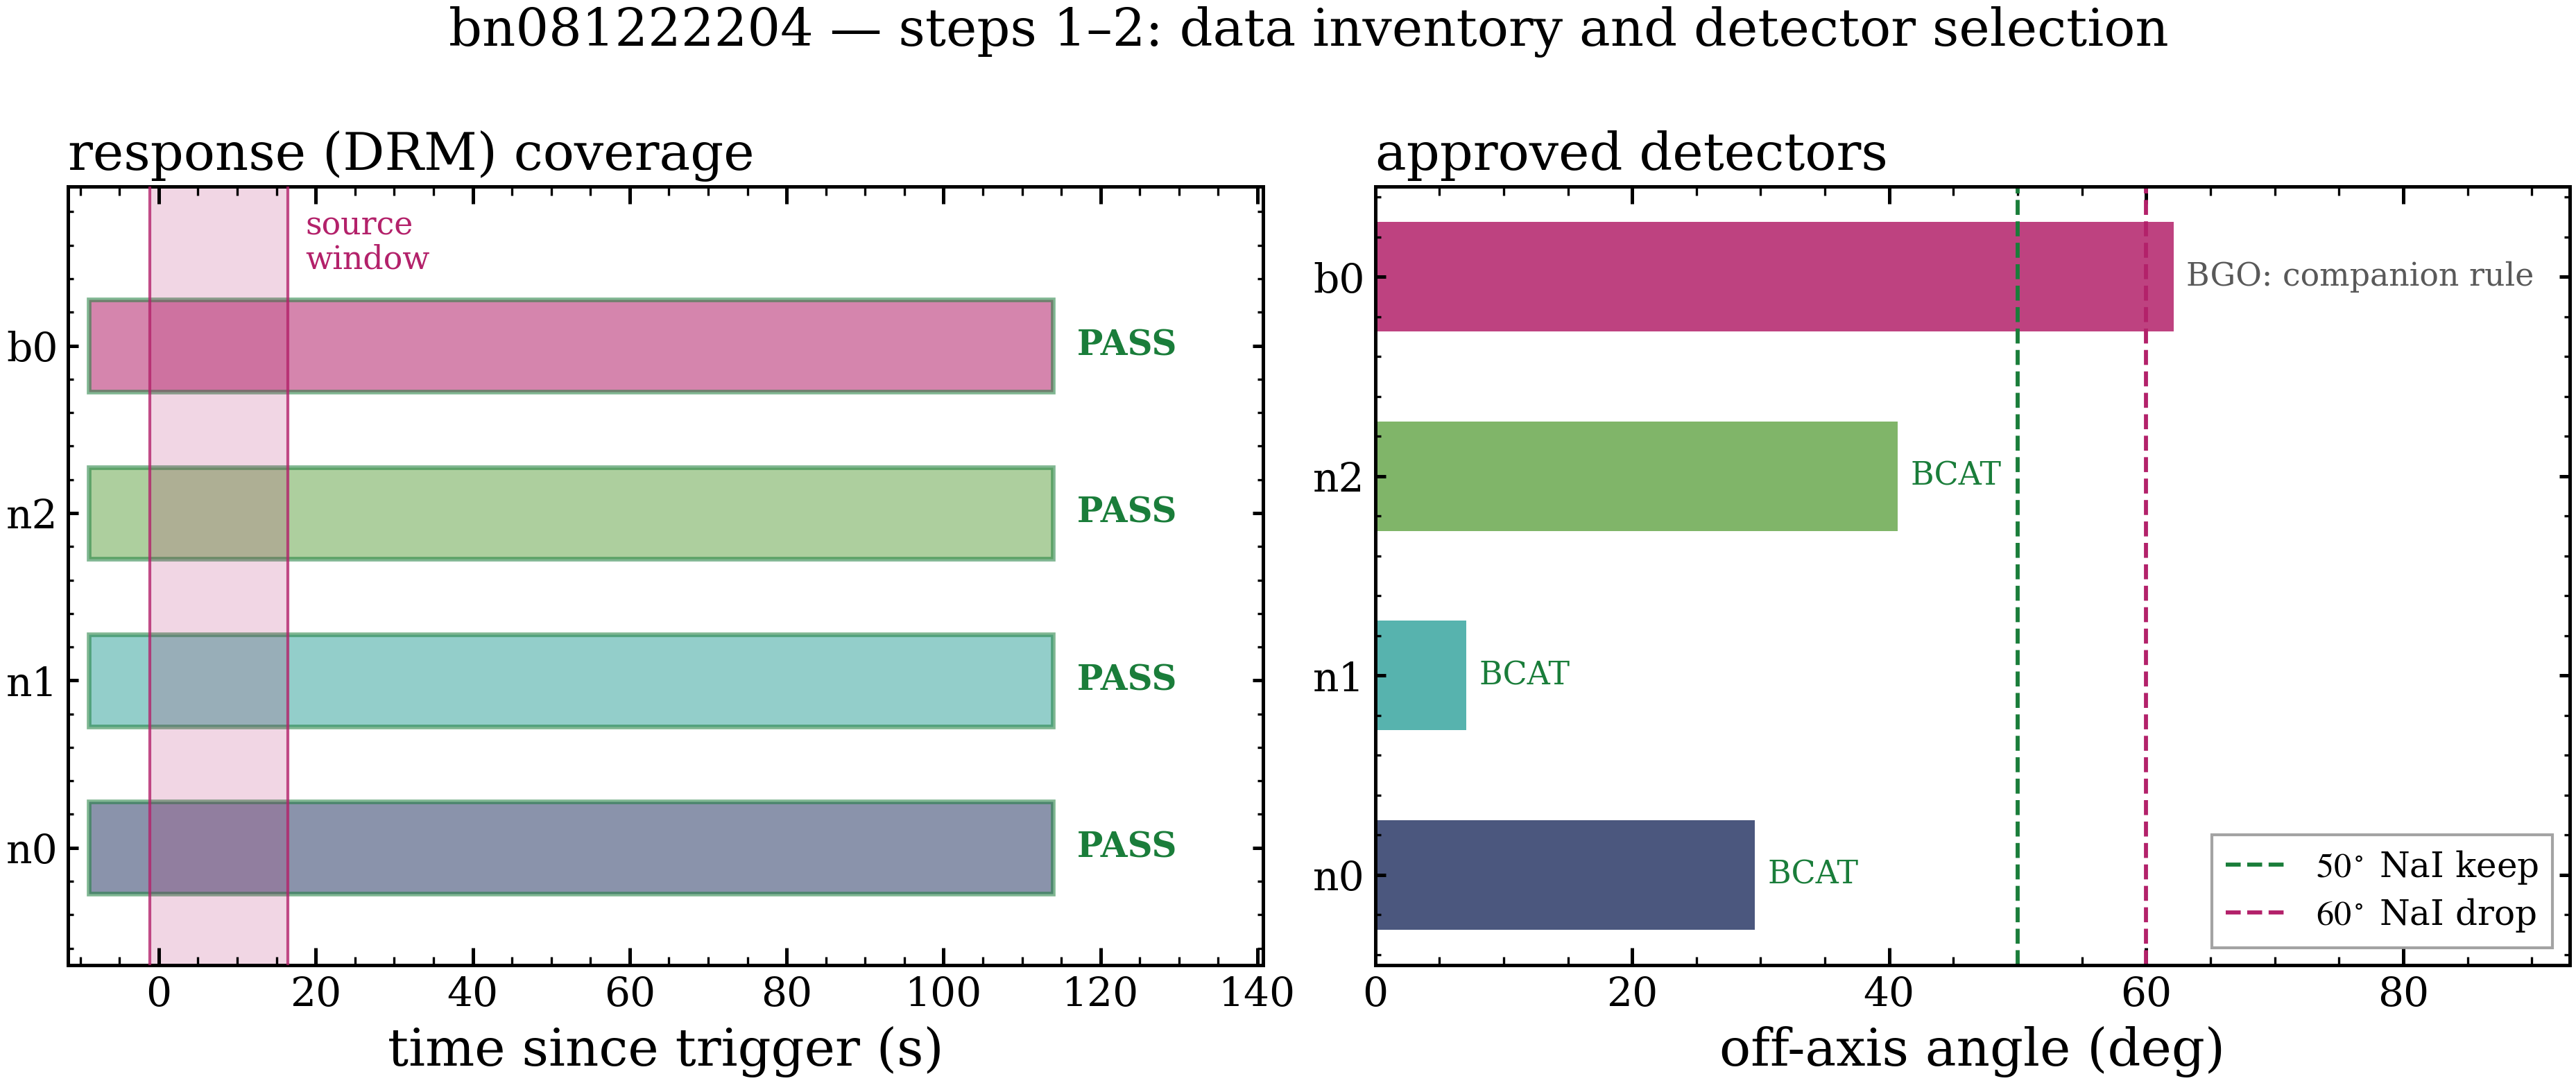
\includegraphics[width=\columnwidth]{figs/bn081222204_step1_inventory.png}
\caption{Detector selection for \grb: source angles with the $50\arcdeg$ rule;
selected detectors $n_0$, $n_1$, $n_2$, $b_1$. \label{fig:step1}}
\end{figure}

\begin{figure}
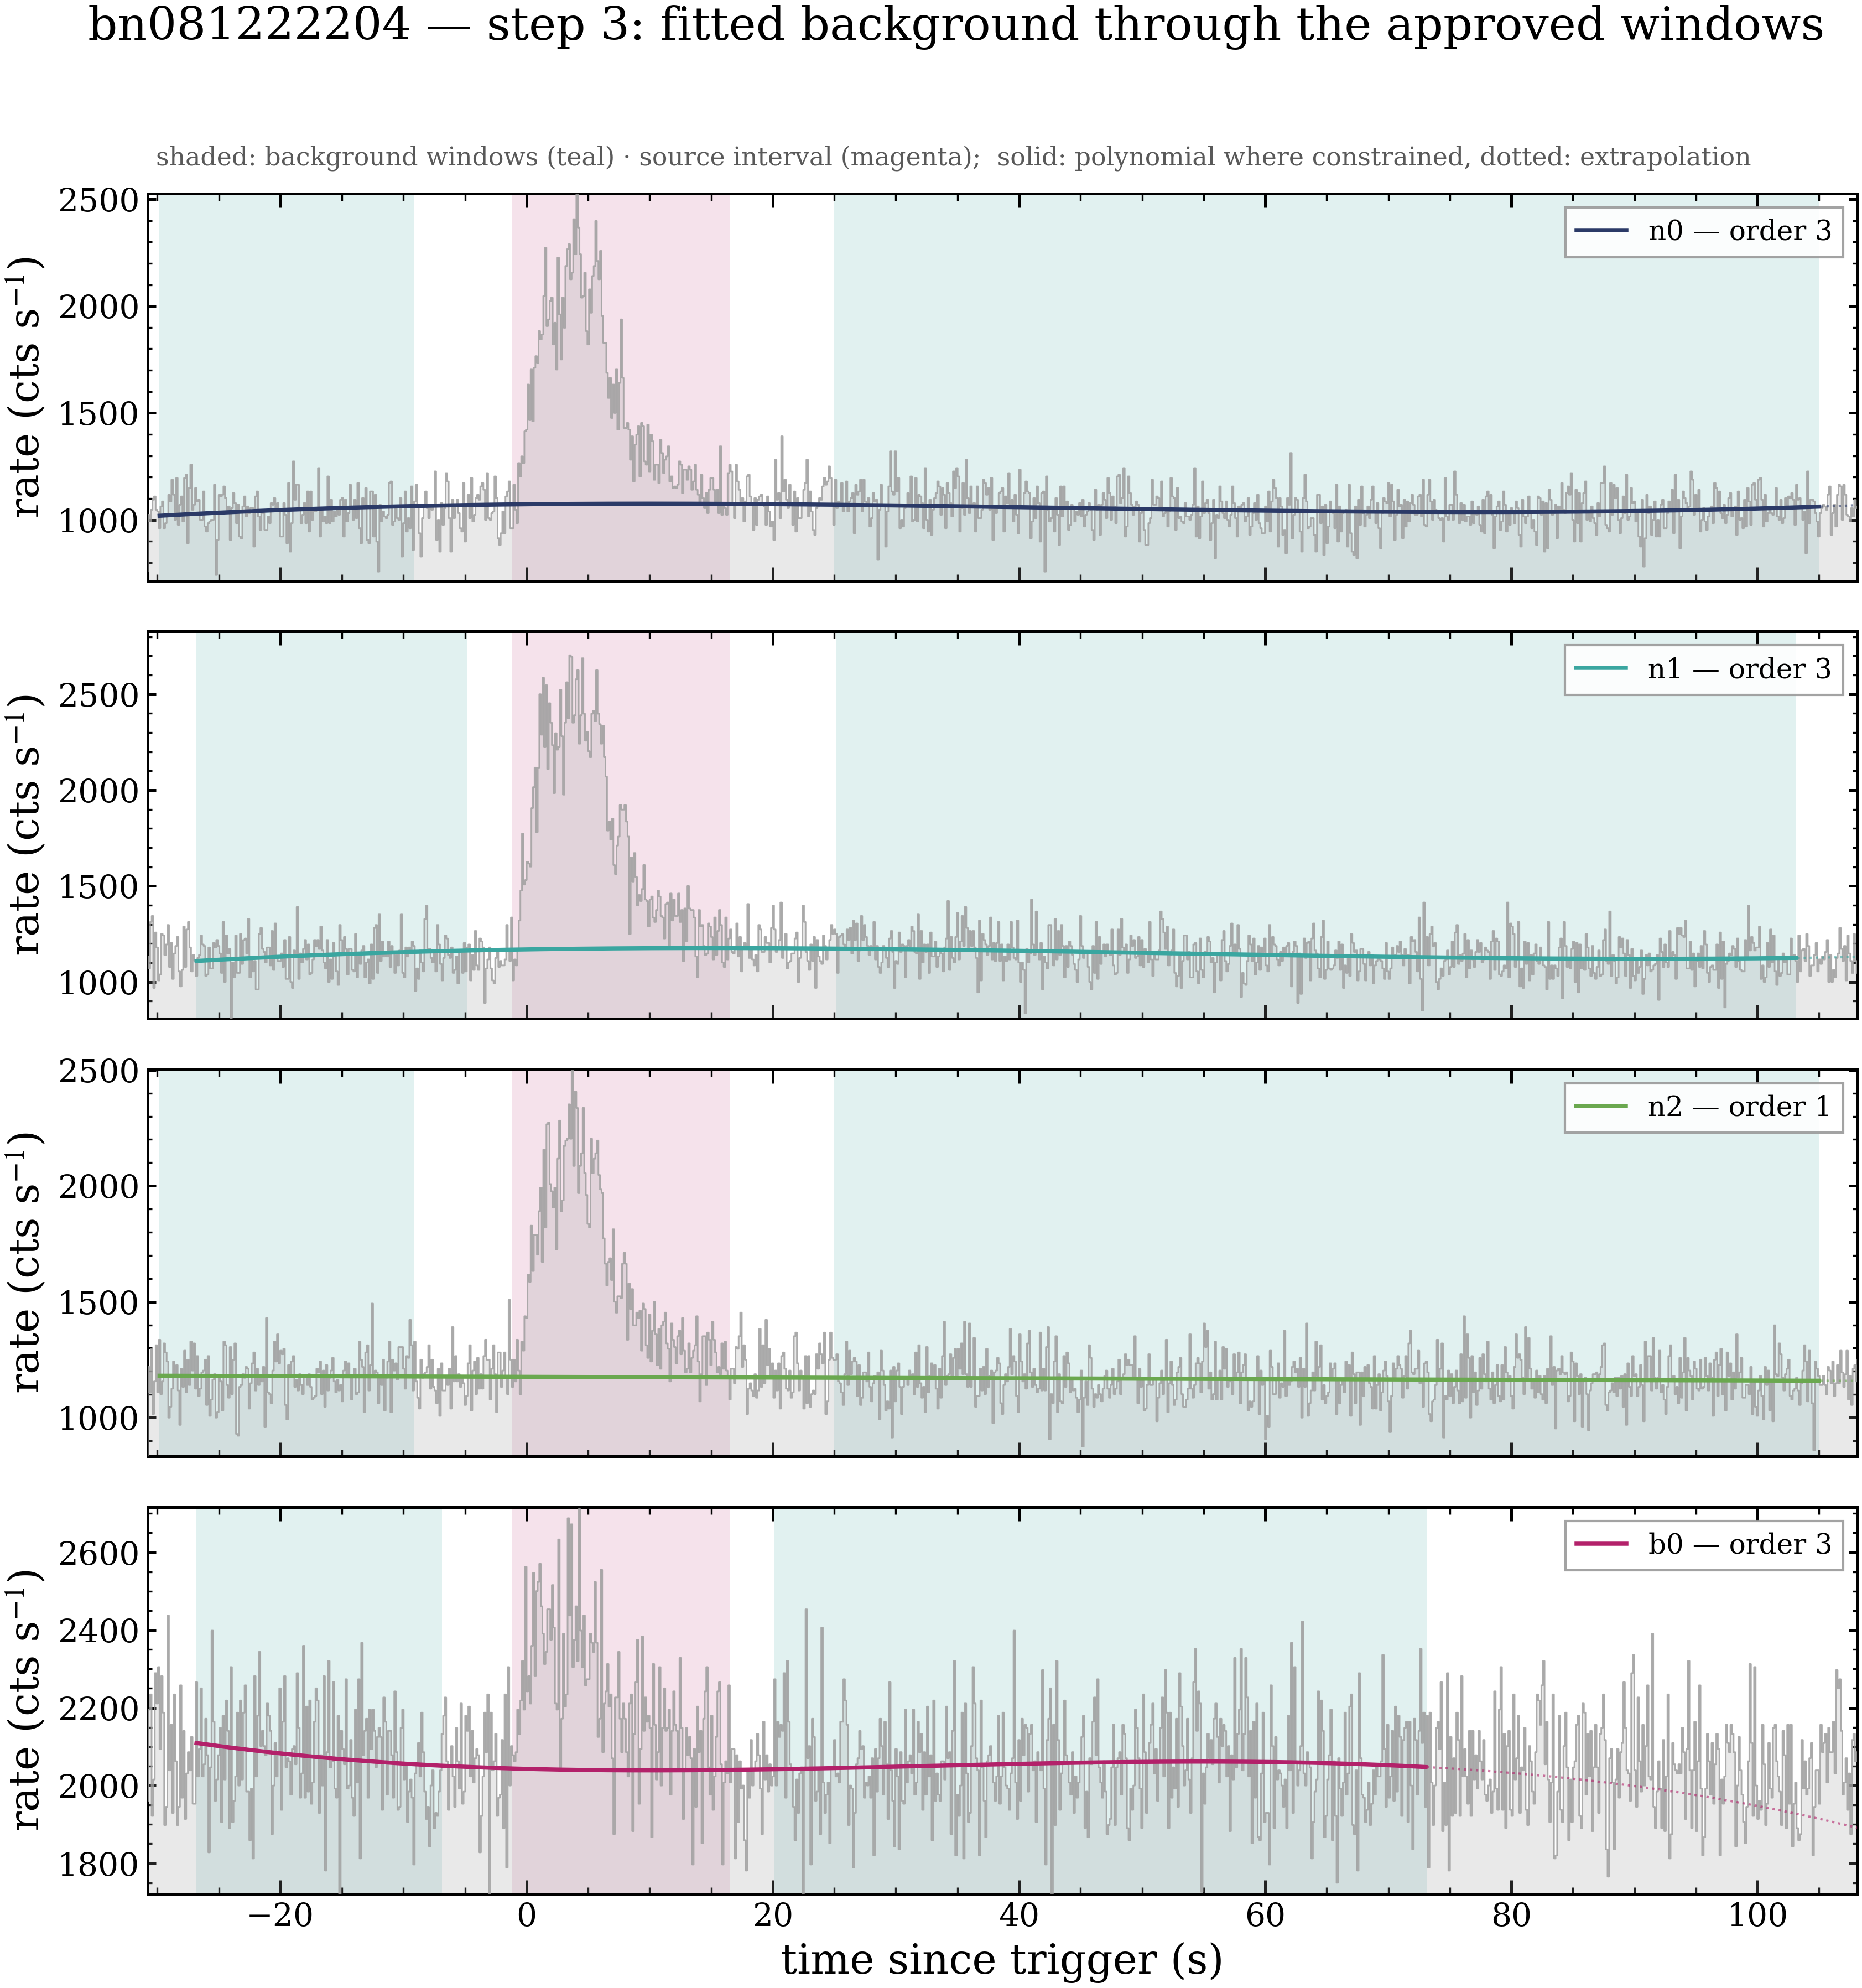
\includegraphics[width=\columnwidth]{figs/bn081222204_step3_background.png}
\caption{Approved background intervals and per-detector polynomial fits.
\label{fig:step3}}
\end{figure}

\begin{figure}
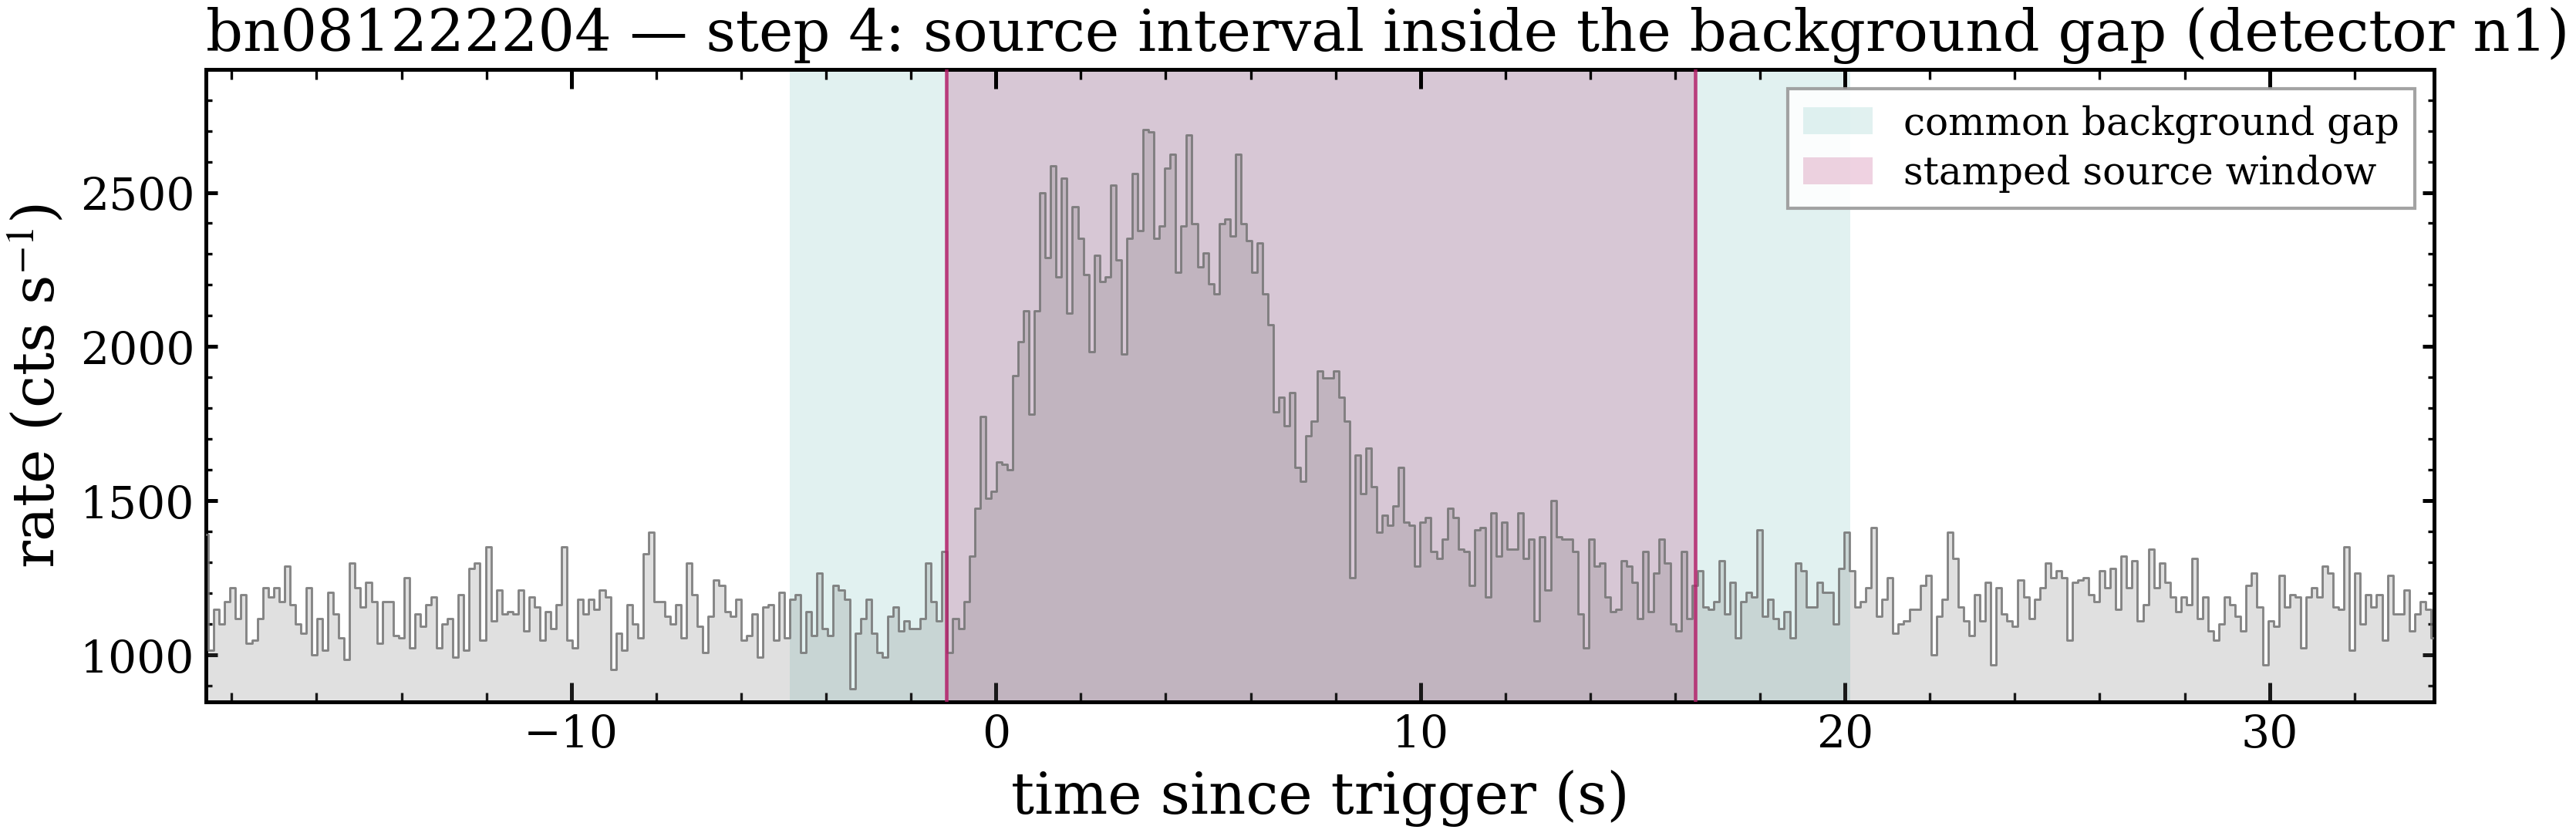
\includegraphics[width=\columnwidth]{figs/bn081222204_step4_source.png}
\caption{Approved source interval over the background-subtracted light curve.
\label{fig:step4}}
\end{figure}

\section{Timing Analysis} \label{sec:timing}

All timing runs on the approved selections, reference NaI $n_1$ for the
temporal chain.

\subsection{Durations} \label{sec:durations}

The windowed duration is $T_{90} = 11.33 \pm 0.32$~s spanning
$[0.53, 11.86]$~s, with the covariance-true Monte Carlo of the campaign
estimator; the interval beyond the source window holds only $2.4\sigma$ of
excess, so unlike burst \#1 this window captures the burst and the duration
is not flagged as a lower limit. The GBM catalog quotes $18.9 \pm 2.3$~s: the
difference is the catalog's own (wider) interval and fluence-space method
versus our windowed count-space measurement, and we flag it for the
literature-comparison step rather than reconcile it by hand. $T_{50} =
4.14$~s. In the rest frame, $T_{90}/(1+z) = 3.01$~s.

Per-band durations (Figure~\ref{fig:step7}) run $11.5 \pm 0.9$~s (8--25~keV)
to $8.1 \pm 0.7$~s (100--350~keV) but follow a single power law poorly
($T_{90} \propto E^{-0.11 \pm 0.04}$, $\chi^2/\mathrm{dof} = 4.3$): three
soft bands are nearly equal before a drop, a caution against per-burst use of
the population-mean band scaling \citep{2013ApJ...763...15Q}.

\begin{figure*}
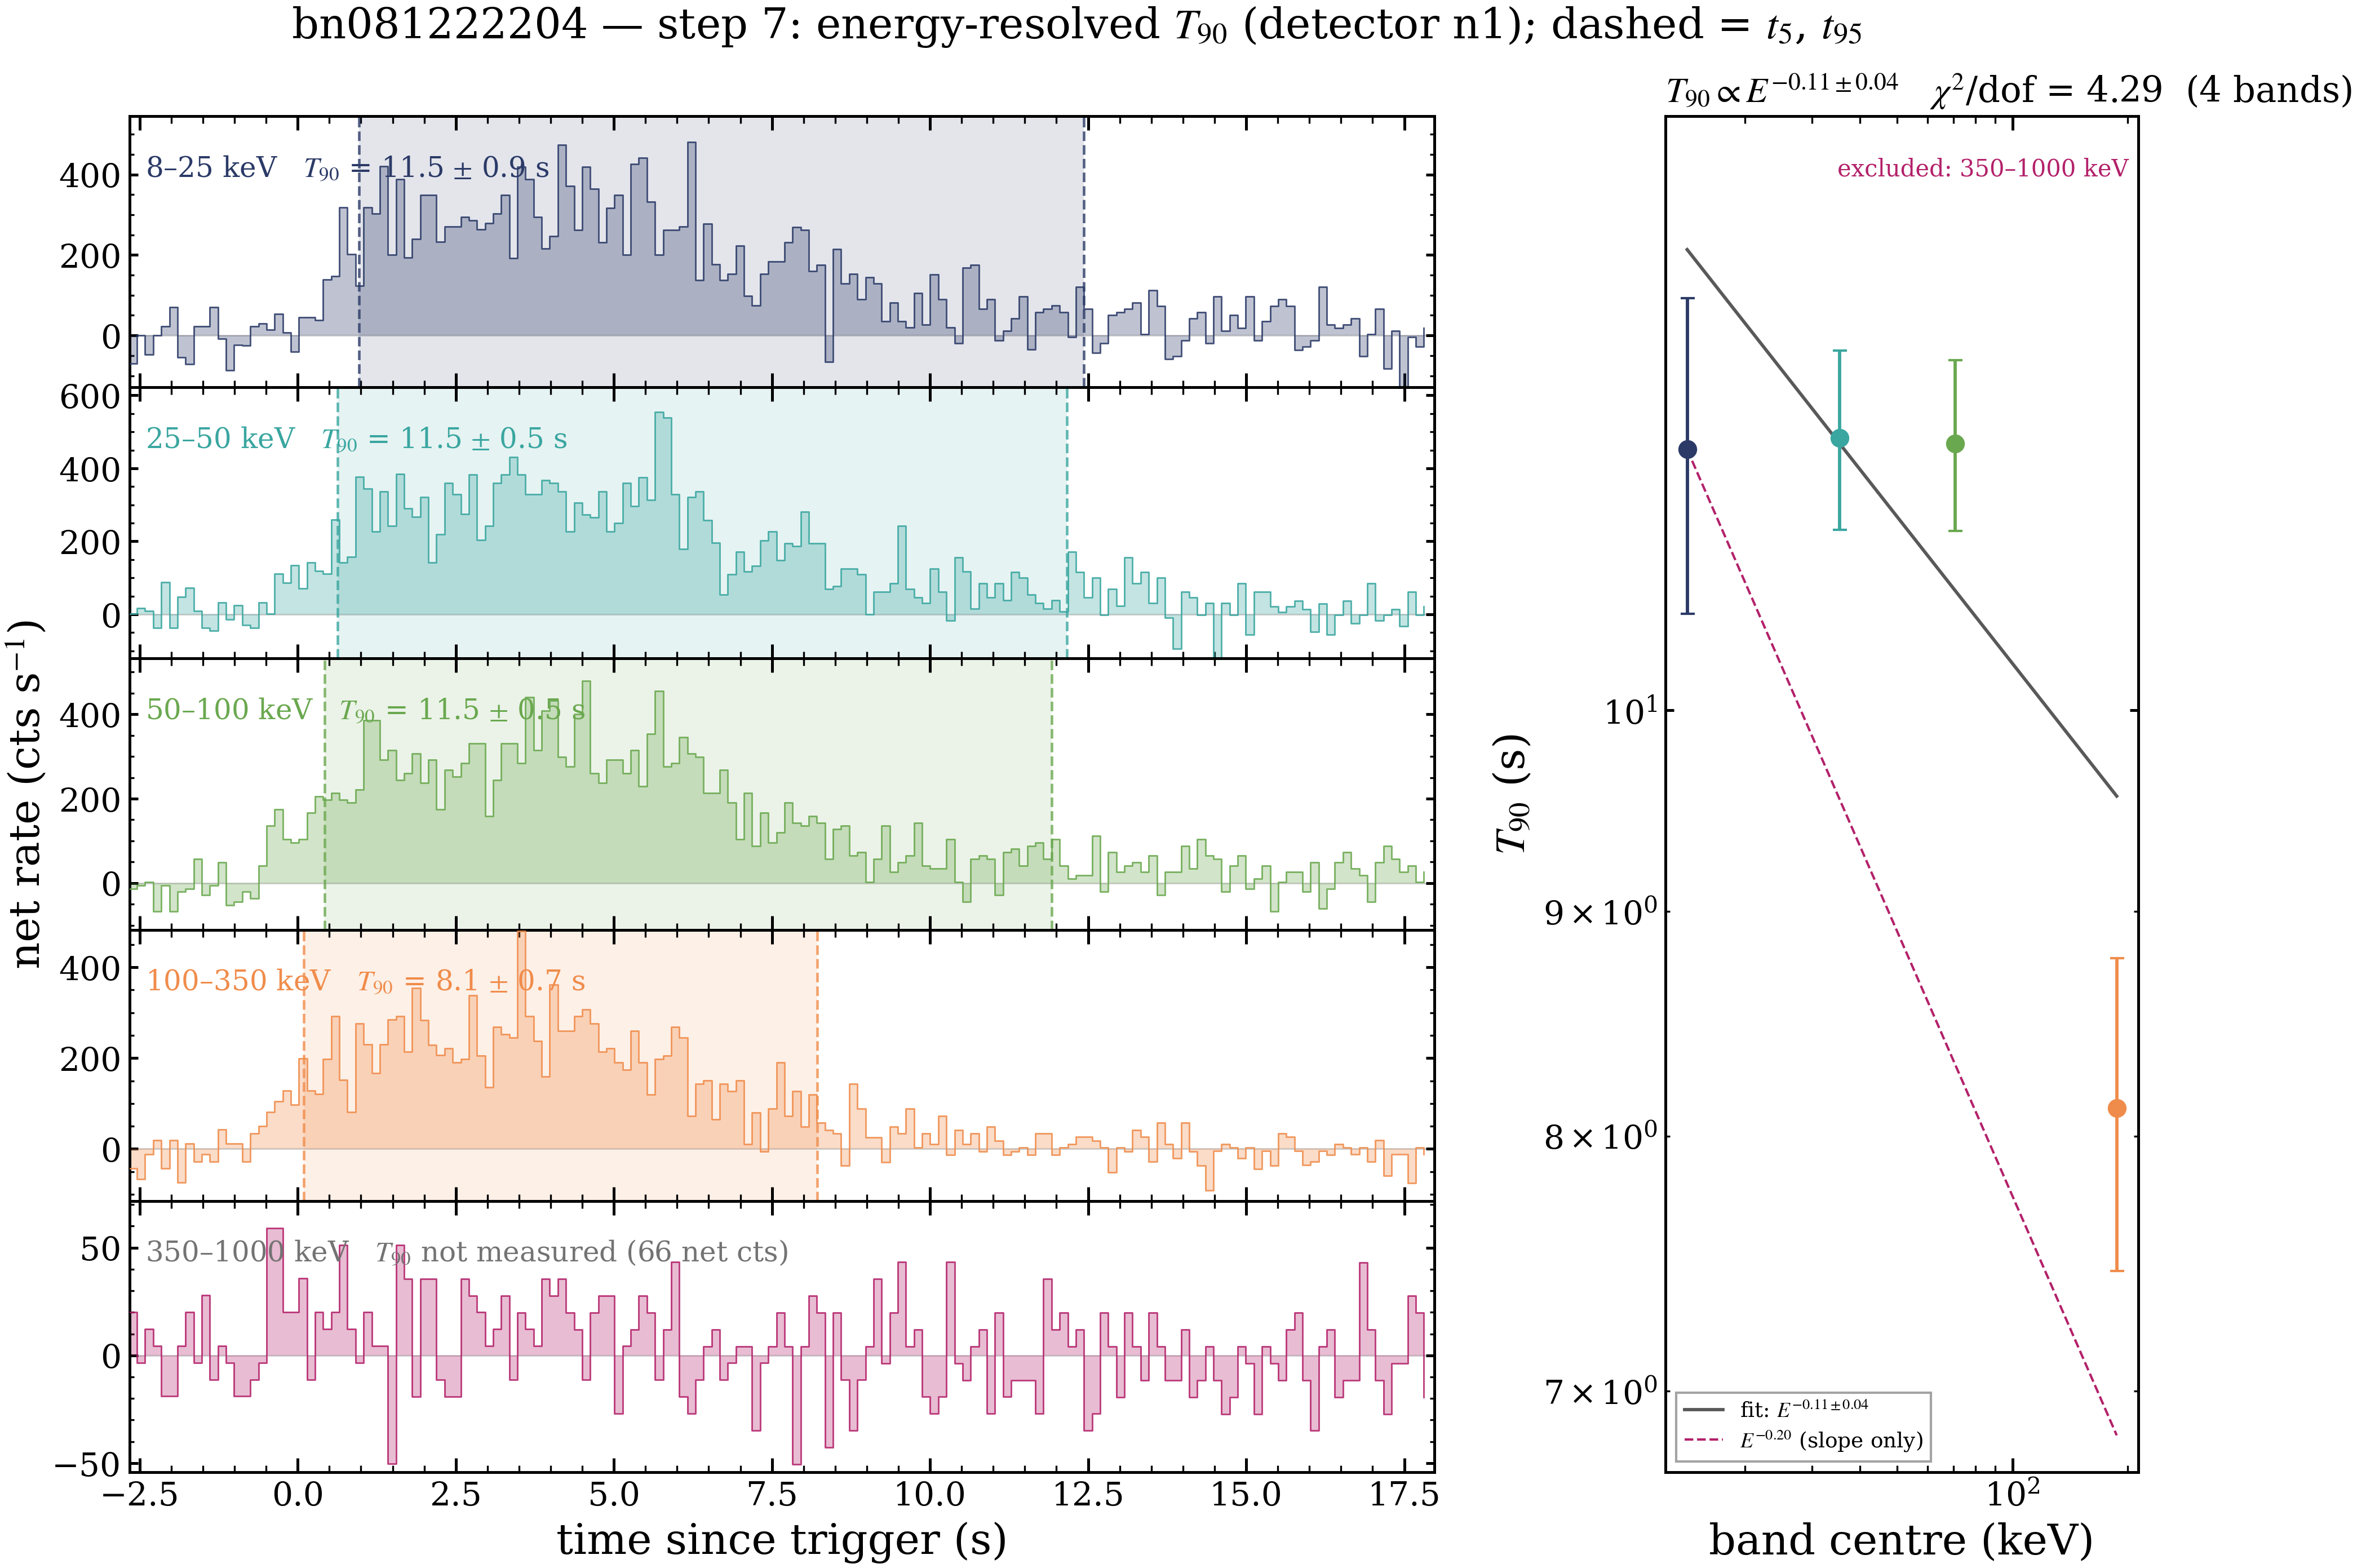
\includegraphics[width=\textwidth]{figs/bn081222204_step7_temporal.png}
\caption{Per-band light curves with individual $T_{90}$ spans (the
350--1000~keV band is excluded for insufficient counts) and the $T_{90}(E)$
relation; the population slope of \citet{2013ApJ...763...15Q} is shown for
reference only. \label{fig:step7}}
\end{figure*}

\subsection{Pulse Shape} \label{sec:pulse}

The \citet{2003ApJ...596..389K} profile wins the shape comparison
($\chi^2_r = 1.09$; Norris 1.12), and the two-sigmoid of
\citet{2025ApJ...991..230G} gives $\varphi = s_l/s_r = 0.263 \pm 0.029$
($R^2 = 0.937$): FRED-like, and statistically indistinguishable from burst
\#1's $\varphi = 0.317 \pm 0.026$ --- two FREDs of consistent asymmetry
(Figure~\ref{fig:pulse}).

\begin{figure}
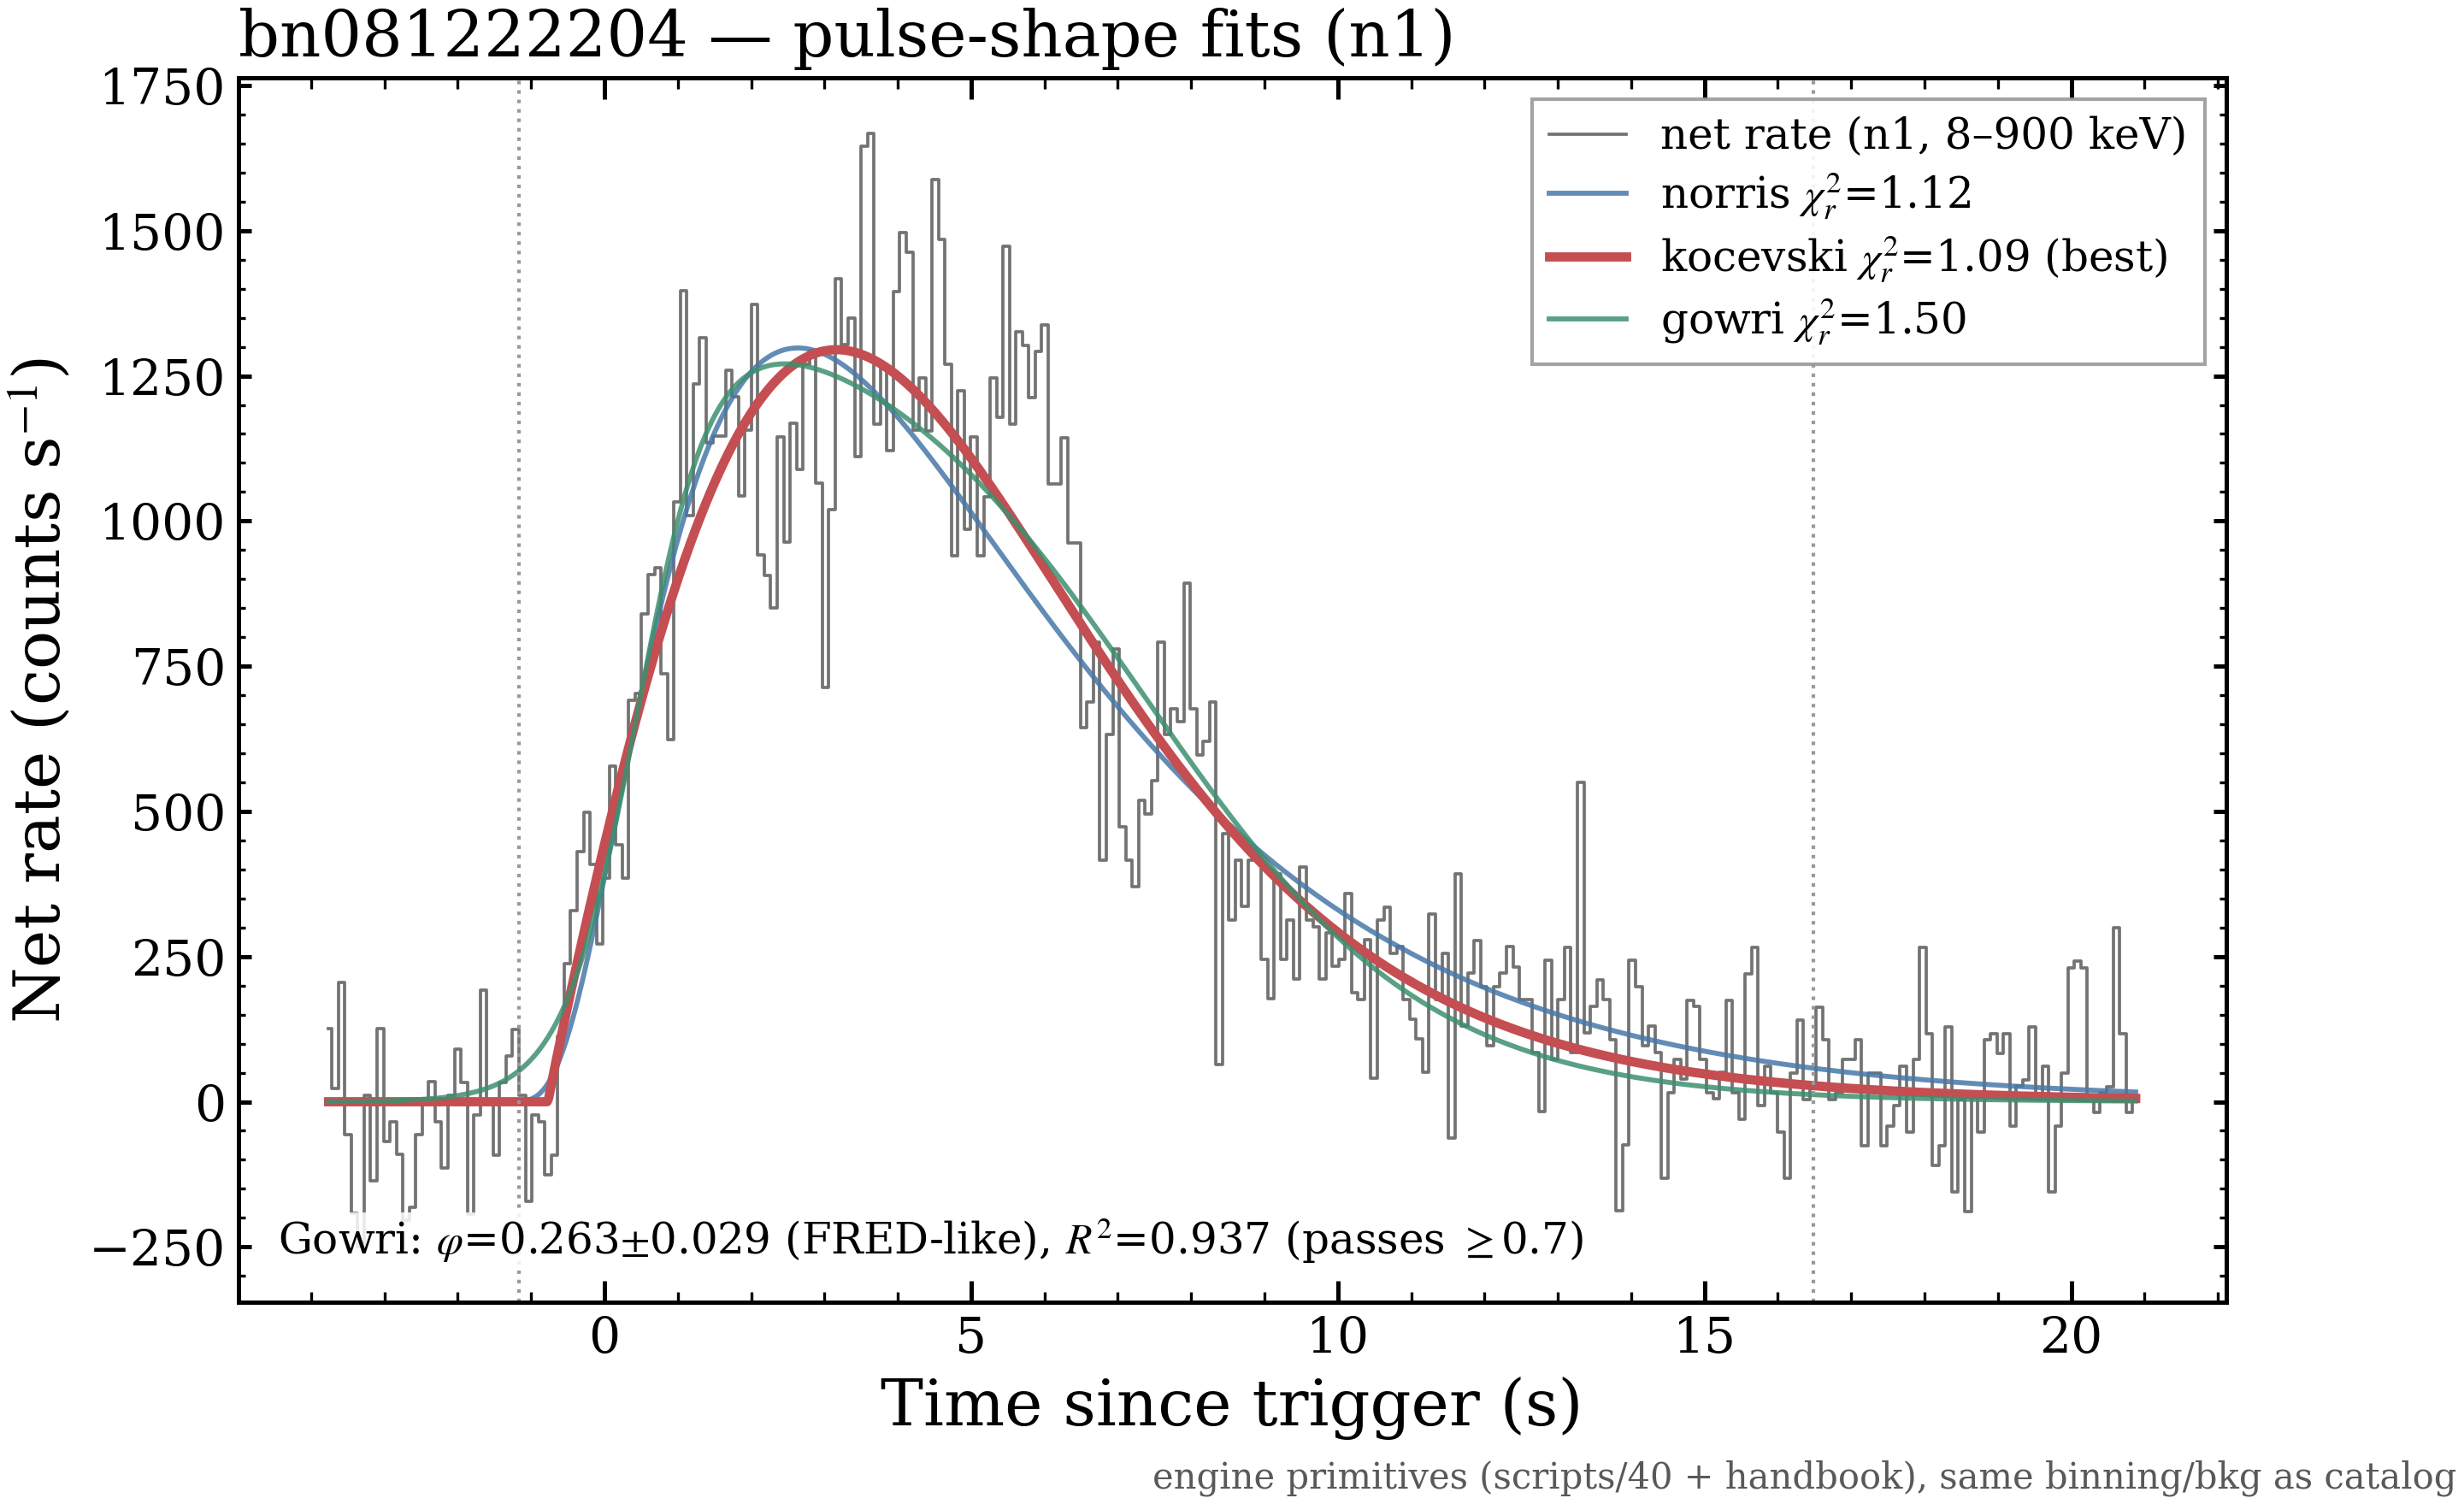
\includegraphics[width=\columnwidth]{figs/bn081222204_step7_pulse.png}
\caption{Pulse-shape fits to the net 8--900~keV light curve; the Kocevski
profile is the $\chi^2_r$ winner. \label{fig:pulse}}
\end{figure}

\subsection{Minimum Variability Timescale} \label{sec:mvt}

Three estimators, three labeled answers (Figure~\ref{fig:mvt}): the windowed
framework of \citet{2026ApJ...999...51B} --- the engine-selected canonical
value --- finds $30.4 \pm 2.1$~ms ($\Delta t = 2$~s segment, detection);
the global CWT \citep{2018ApJ...864..163V} returns $215 \pm 17$~ms, which we
note is grid-quantized (the discrete wavelet-scale ladder makes cross-burst
CWT values cluster on rungs; the quoted error is grid spacing); and the Haar
cross-check \citep{2014ApJ...787...90G} yields only an upper limit
($< 1.02$~s), drawn as one. In the rest frame the canonical MVT is
$\approx 8$~ms --- a direct engine-variability timescale at $z = 2.77$.

\begin{figure}
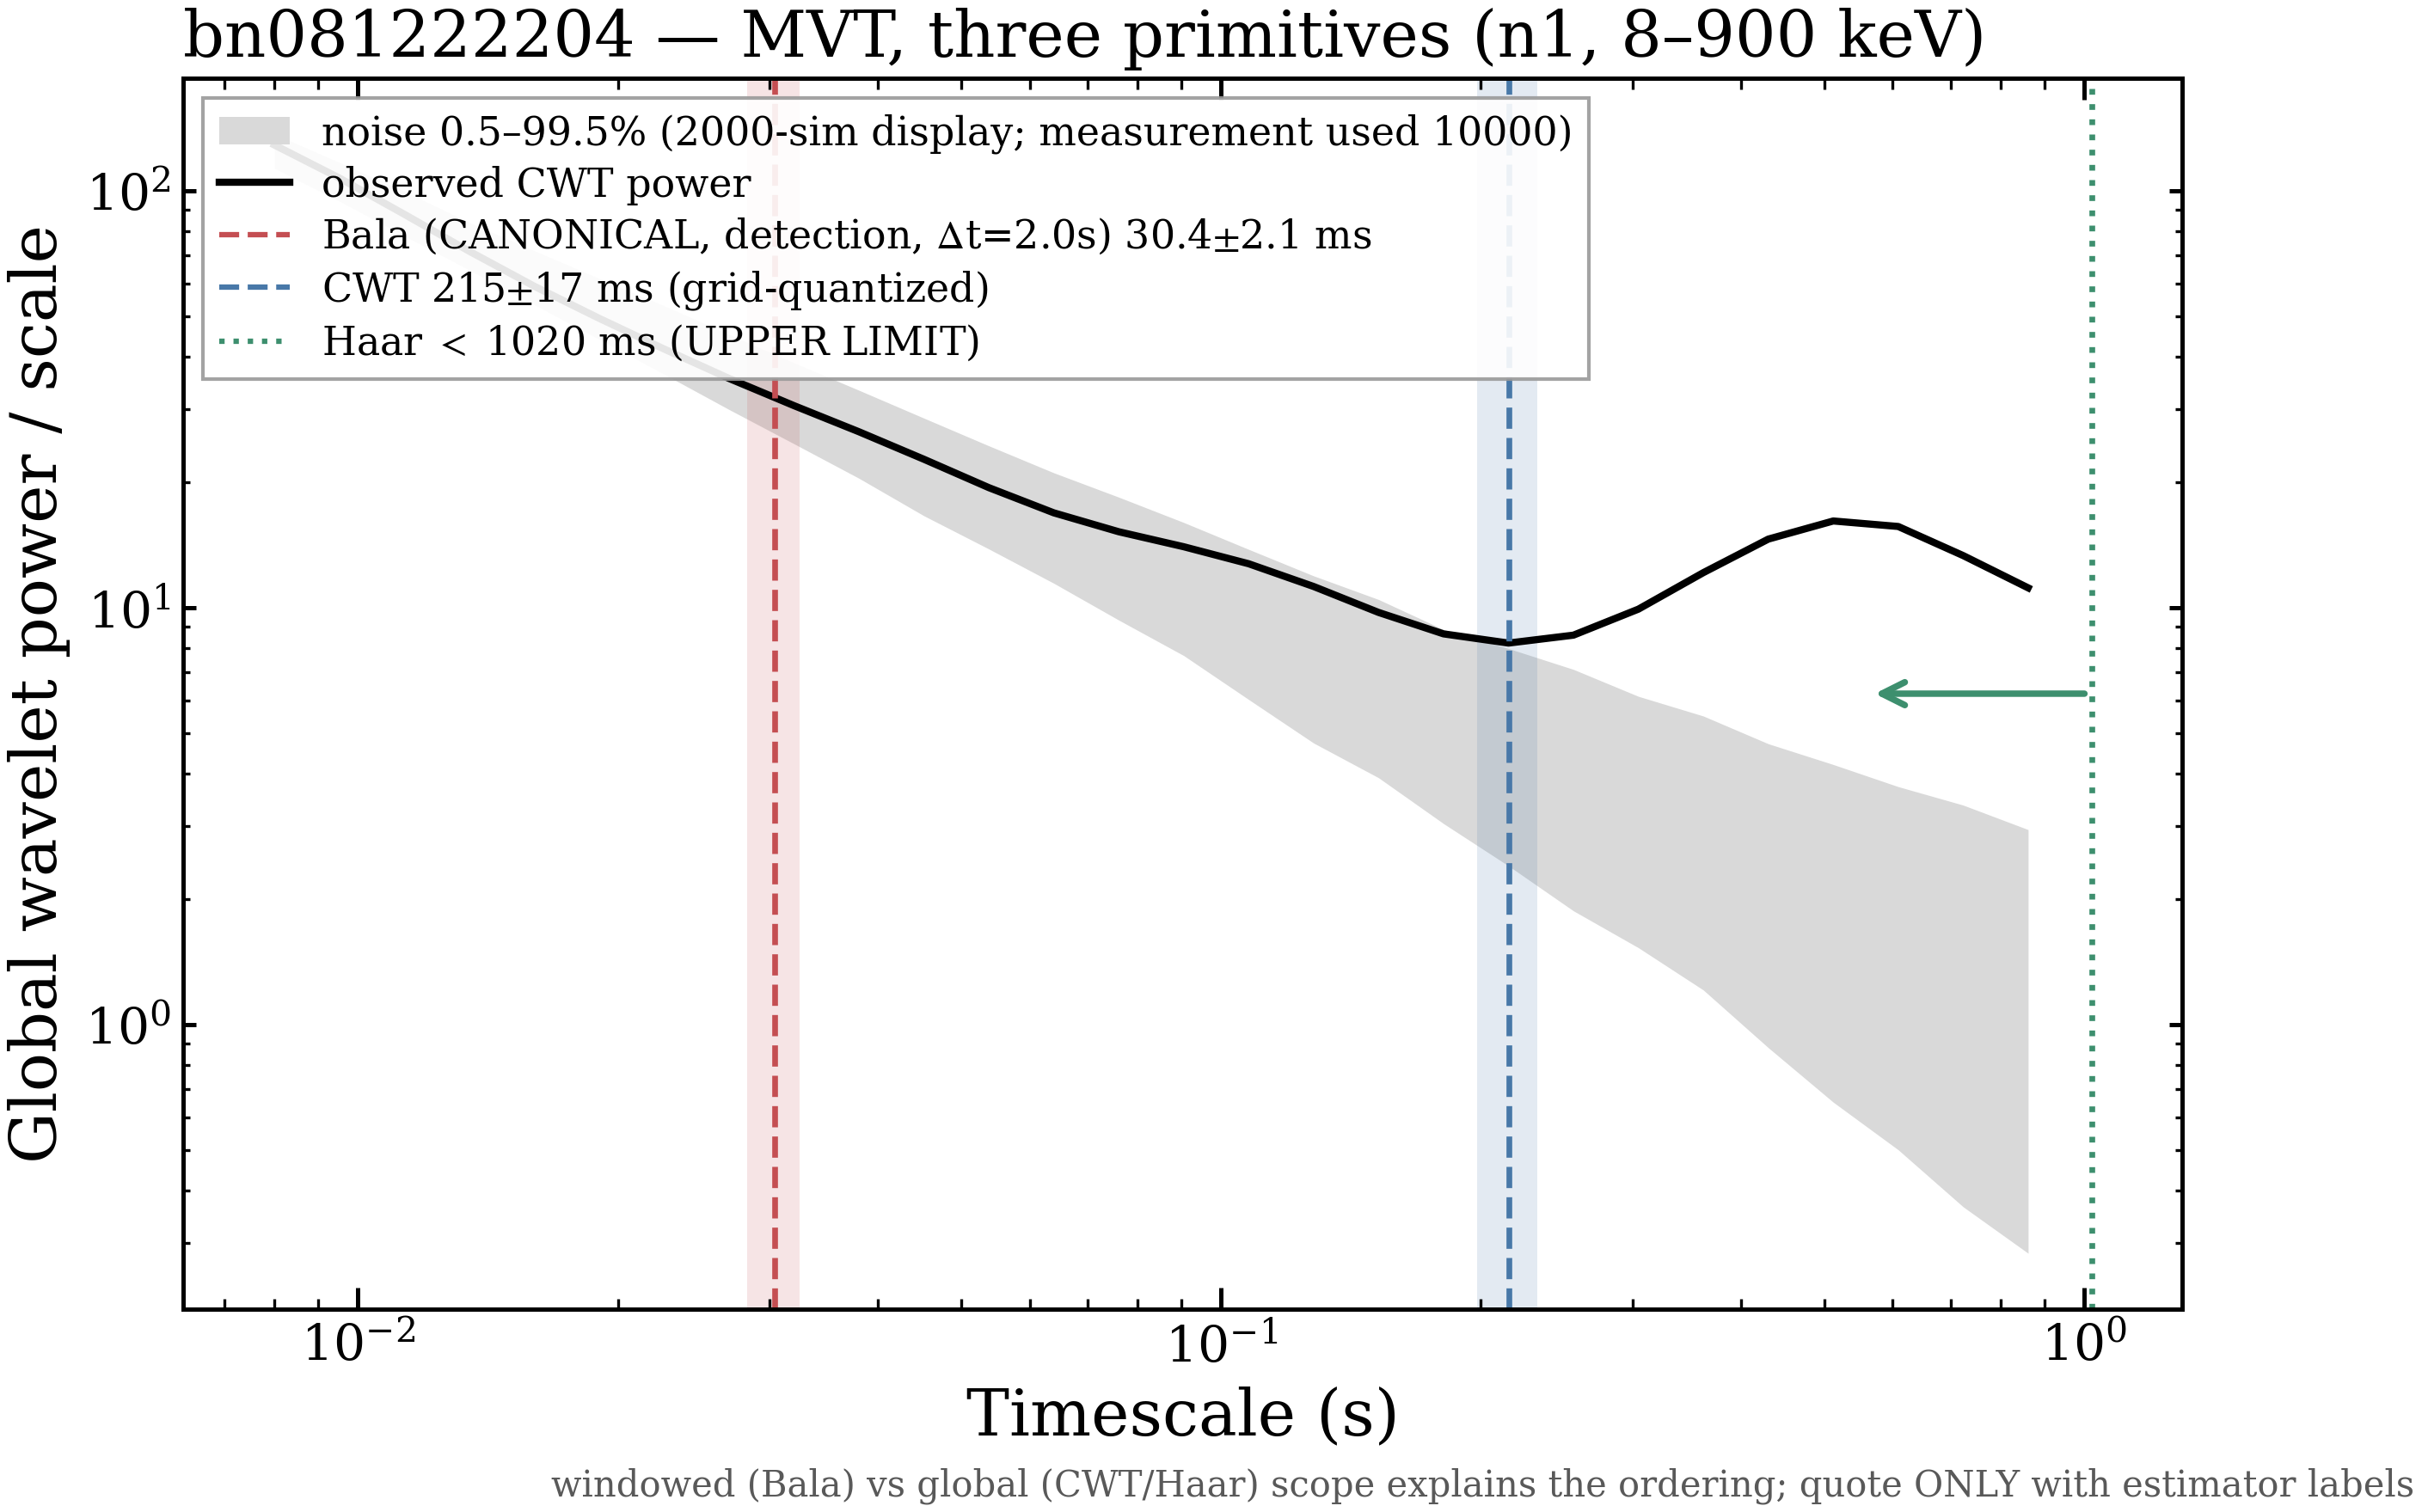
\includegraphics[width=\columnwidth]{figs/bn081222204_step7_mvt.png}
\caption{Global CWT power spectrum against its Poisson floor with all three
MVT estimators marked; the Haar value is an upper limit and is rendered as
one. Windowed-vs-global scope explains the ordering. \label{fig:mvt}}
\end{figure}

\subsection{Spectral Lag} \label{sec:lag}

Using the DCCF \citep{1997ApJ...486..928B} with an asymmetric-Gaussian peak
model \citep{2015MNRAS.446.1129B} and flux-randomization Monte Carlo
\citep{1998PASP..110..660P}, we scan the fit window around the correlation
peak (the peak position is the deliverable; the window spread enters as a
systematic): $\tau = 0.474^{+0.171}_{-0.269} \pm 0.377_{\rm win}$~s, soft
lagging hard \citep{1996ApJ...459..393N,2010ApJ...711.1073U}, with a
$30\sigma$ correlation peak (Figure~\ref{fig:lag}). The window systematic
dominates: this burst's flat-topped DCCF localizes its peak only to
$\pm 0.4$~s, and any use of this lag must carry that width. In lag--width
terms, $\tau/T_{90} \approx 0.042$ --- half of burst \#1's 0.085: two bursts
into the campaign, the lag--width ratio is already not constant. Rest-frame
lag $\approx 0.13$~s.

\begin{figure}
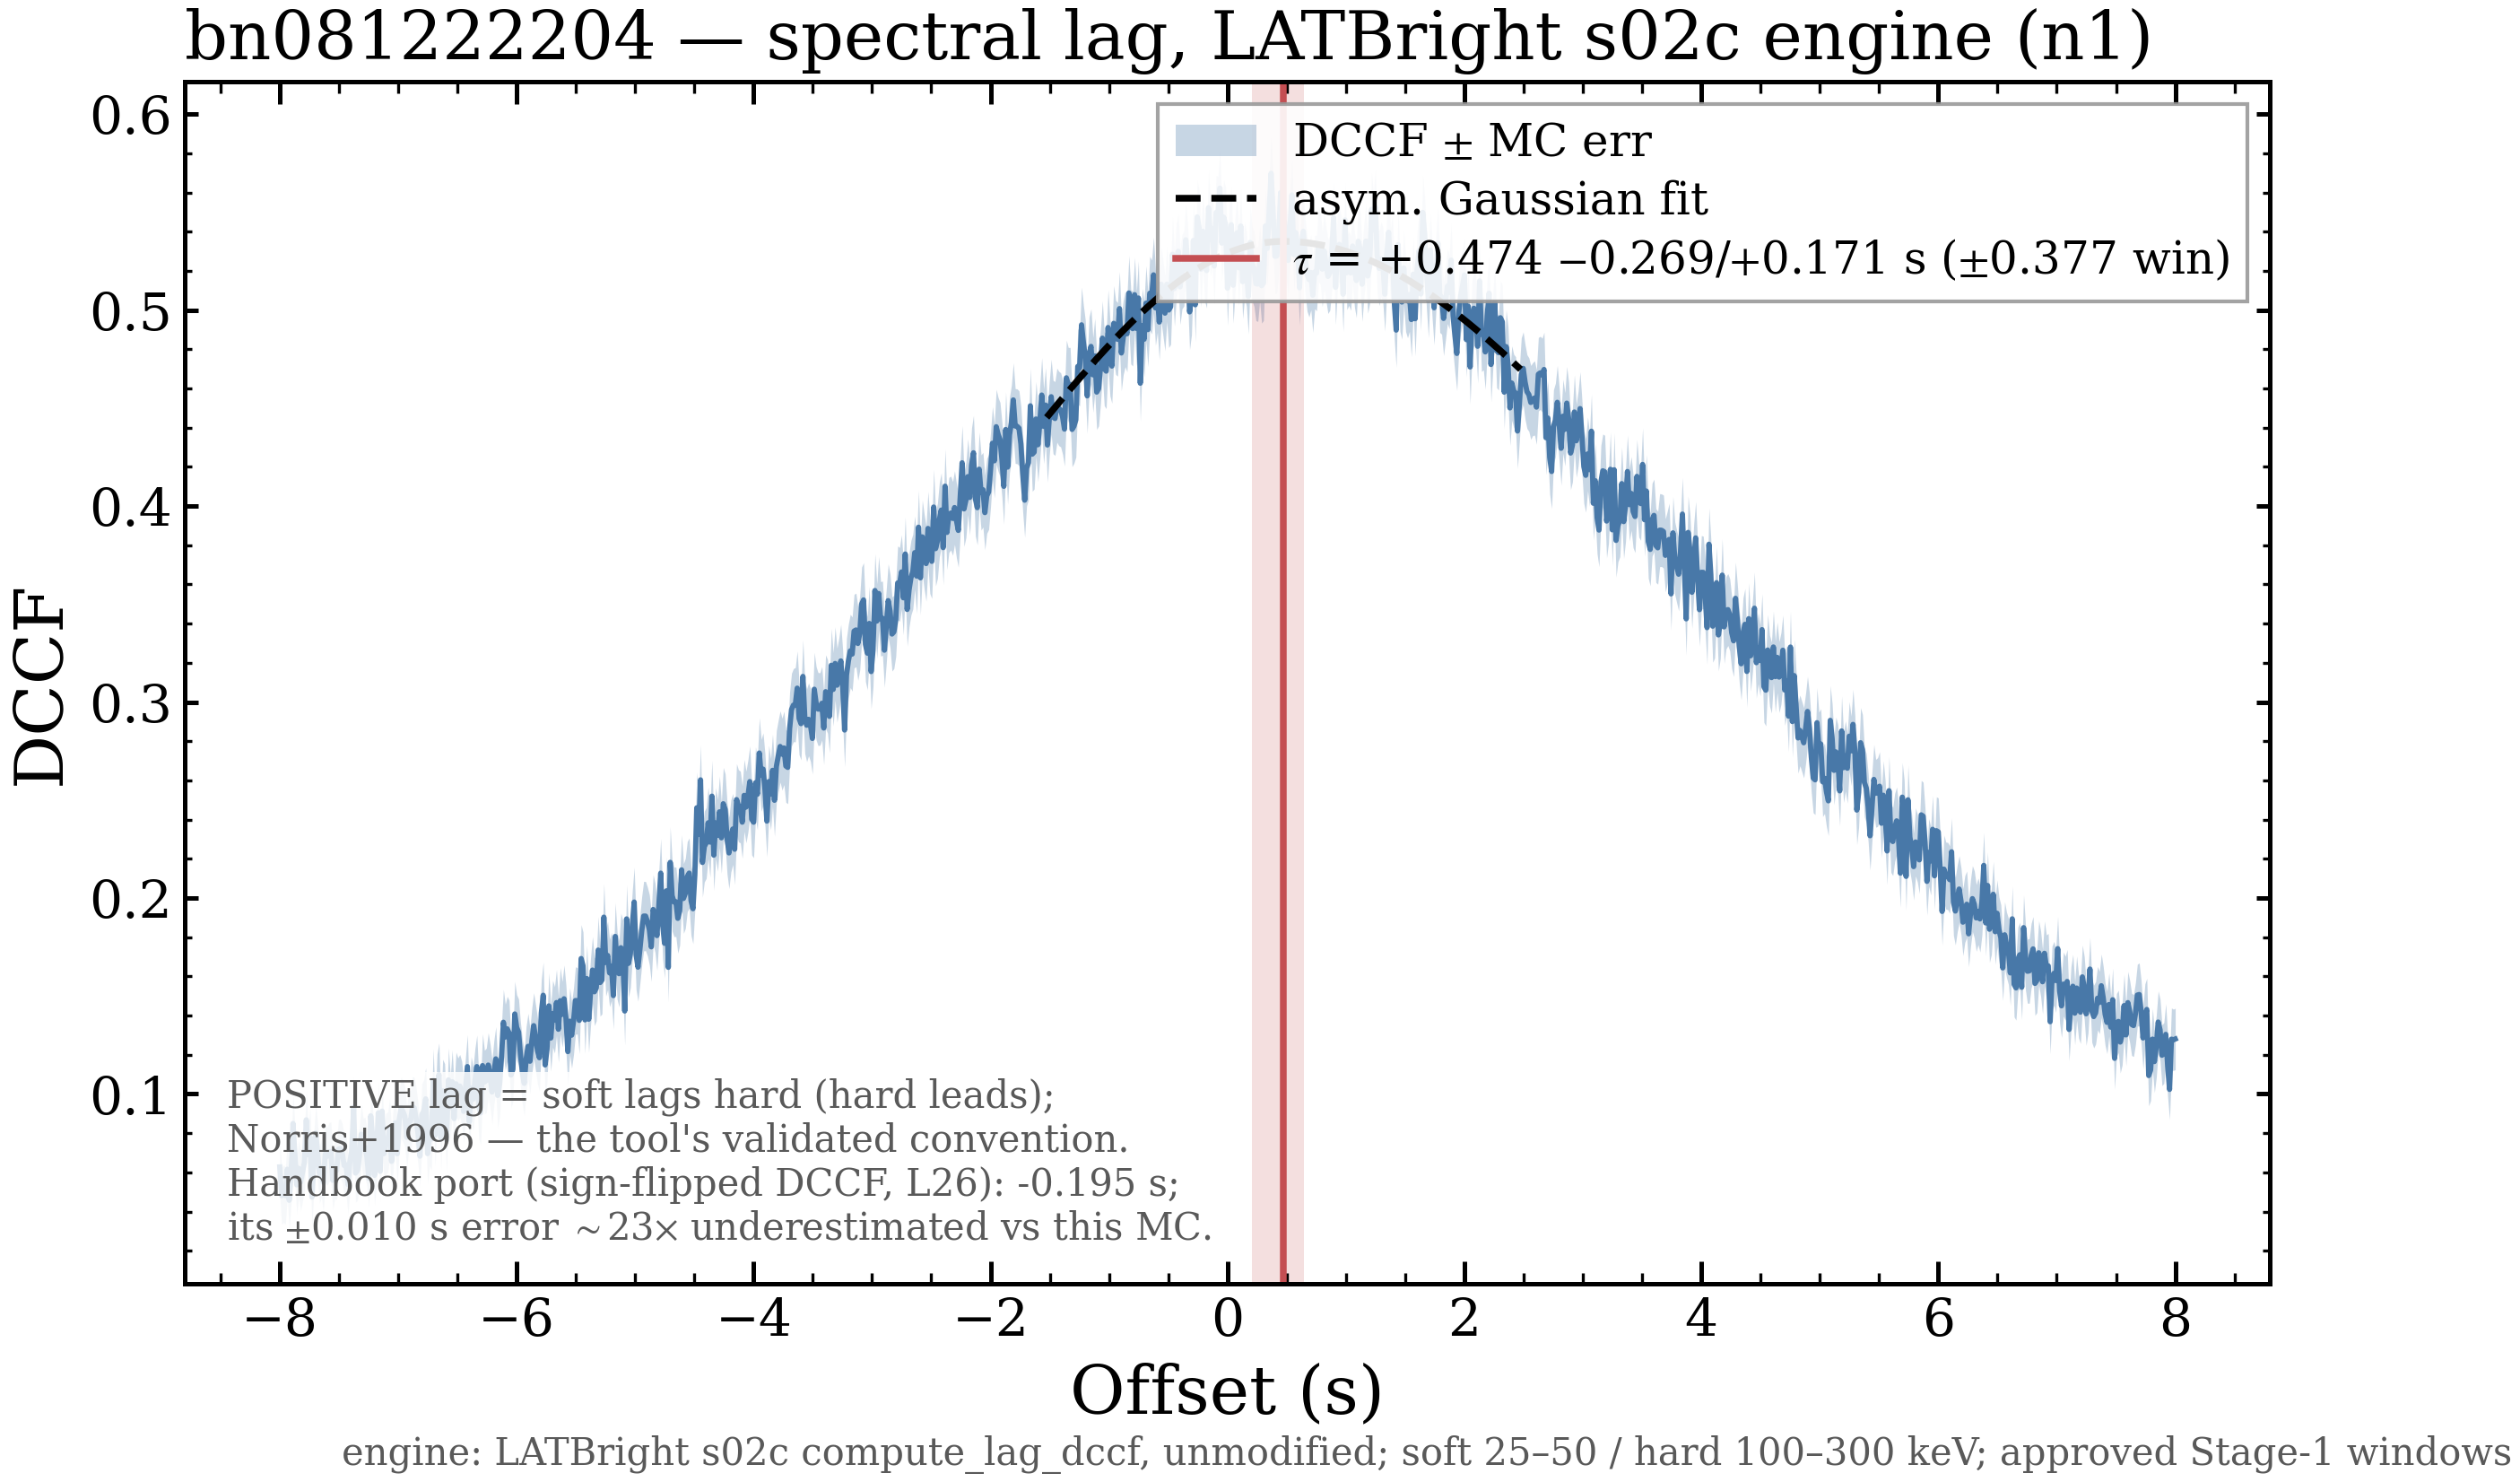
\includegraphics[width=\columnwidth]{figs/bn081222204_step7_lag_latbright.png}
\caption{DCCF of the 25--50 vs.\ 100--300~keV light curves with the
window-scanned asymmetric-Gaussian peak fit; the legend carries both the
Monte-Carlo errors and the window systematic. \label{fig:lag}}
\end{figure}

\section{Time Binning} \label{sec:binning}

Bayesian blocks \citep{2013ApJ...764..167S} through 3ML
\citep{2015arXiv150708343V} with the campaign's $S \ge 10$ significance merge
yield six bins spanning $-0.47$ to $14.57$~s (Figure~\ref{fig:step5}).

\begin{figure}
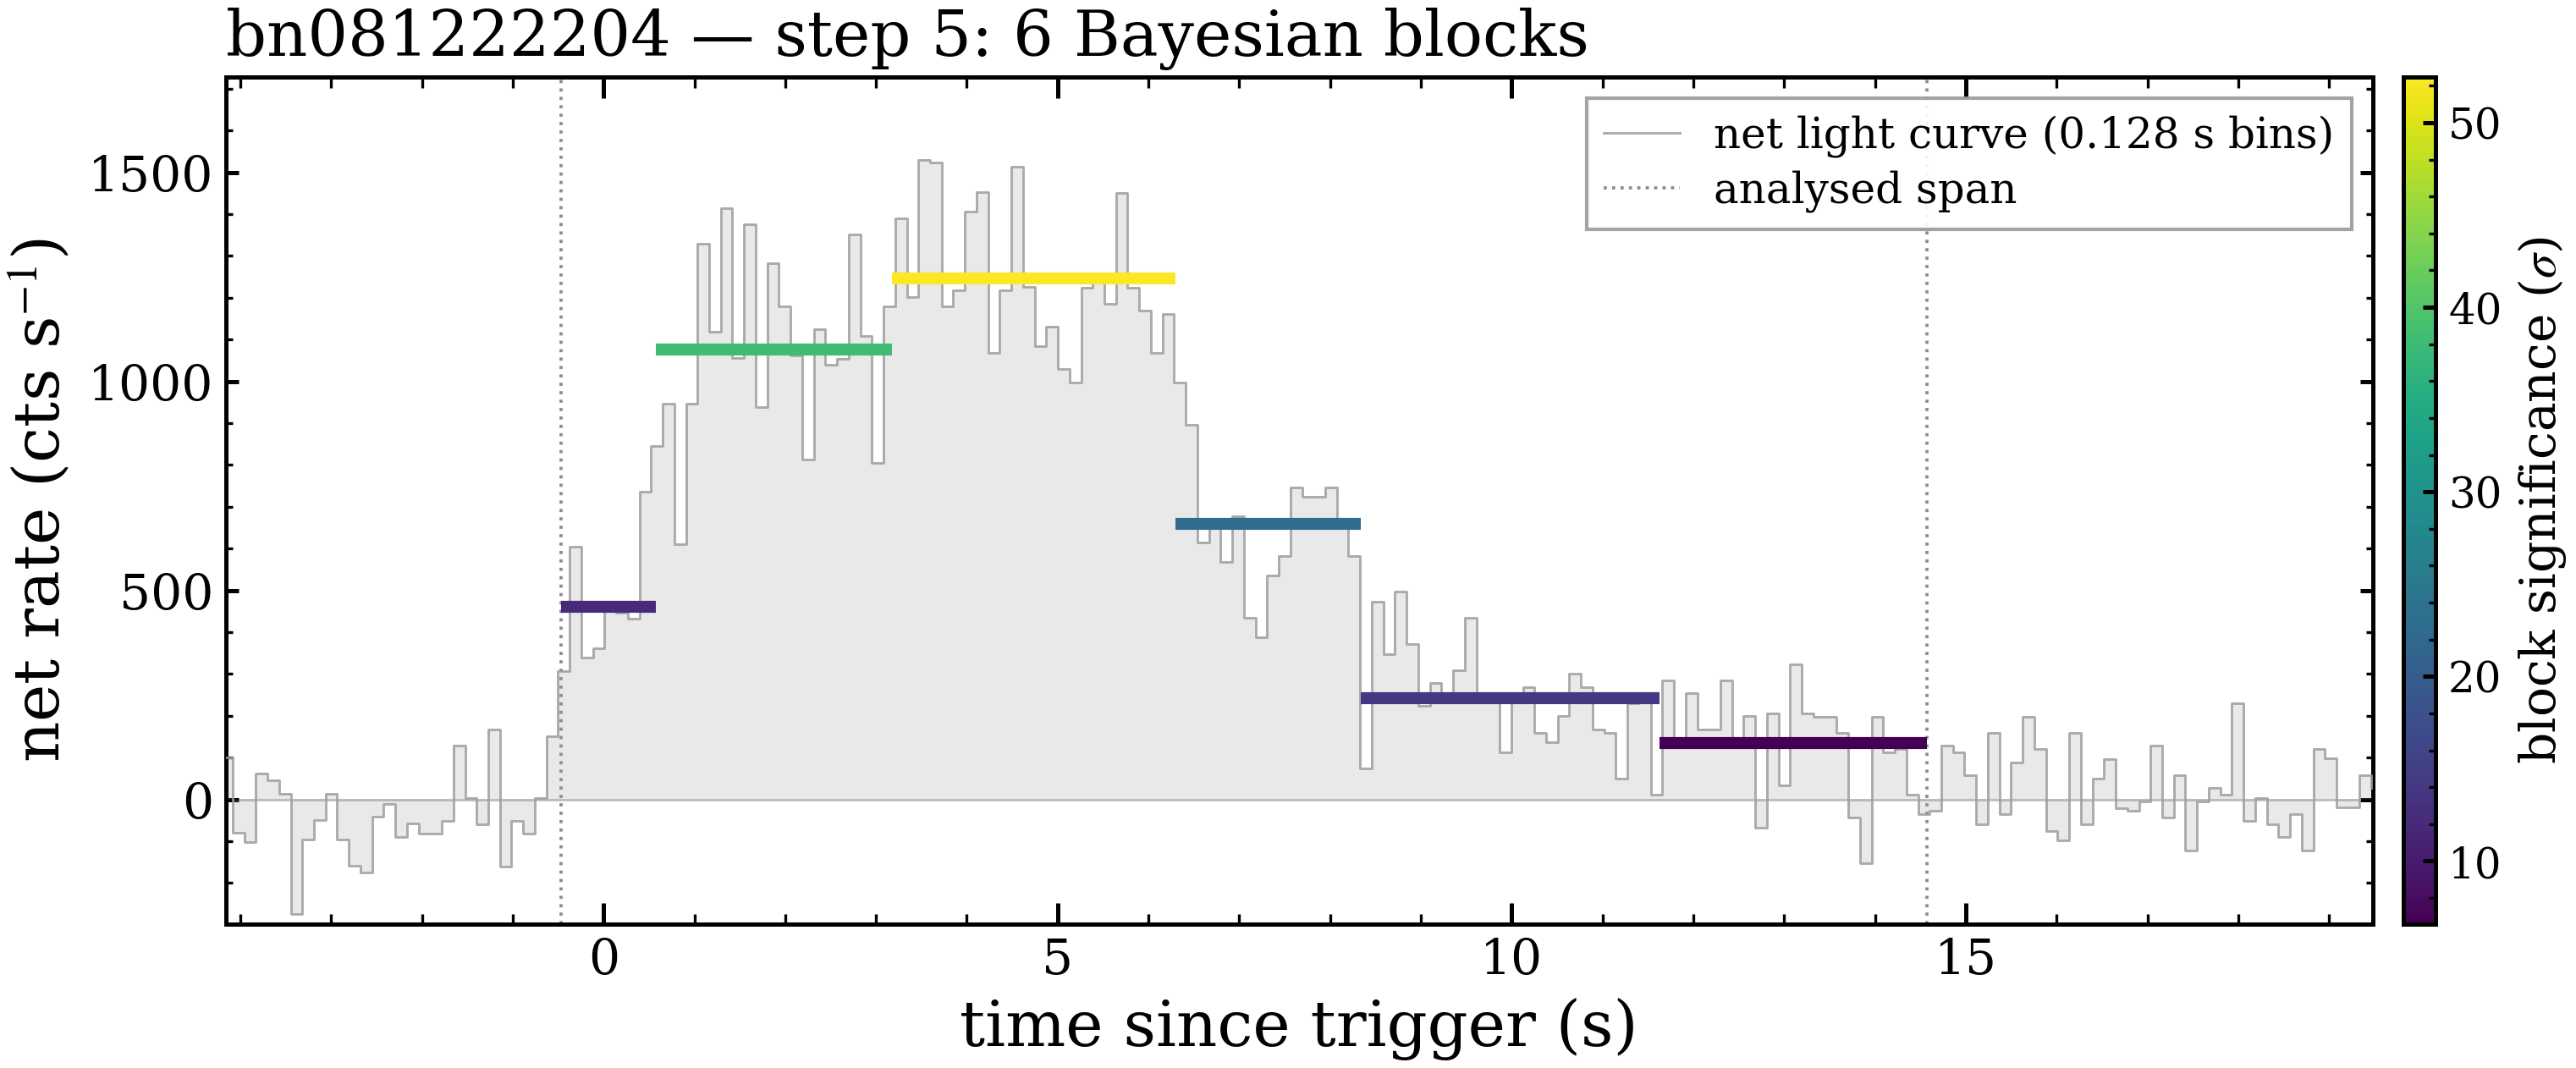
\includegraphics[width=\columnwidth]{figs/bn081222204_step5_binning.png}
\caption{Bayesian-block decomposition and the six spectroscopy bins.
\label{fig:step5}}
\end{figure}

\section{Time-Resolved Spectroscopy} \label{sec:spectra}

\subsection{Method and Panel Provenance} \label{sec:specmethod}

We fit the campaign's 24 spectral models in each bin and the integrated
spectrum ($\pgstat$ minimization, AIC selection
\citep{1974ITAC...19..716A}; $\Delta\mathrm{AIC} < 2$ reported as ties).
Every (model, bin) pair is rendered under the campaign's no-model-dropped
rule in one of three provenance tiers: live-verified (the display fit
reproduces the stored solution to $|\Delta\mathrm{AIC}| \le 0.1$), frozen
replay (the stored solution evaluated exactly, stamped, no error band), or a
labeled structural refusal (none occurred: 168/168 panels exist). One model
required an engine retry in the faintest bin (a transient multistart
failure); it converged on the second attempt and its row was merged. The
time-integrated winner has $\pgstat/\mathrm{dof} = 5593.9/460$.

\subsection{Results} \label{sec:specresults}

Table~\ref{tab:winners} lists winners and parameters.
Figure~\ref{fig:sedtint} shows the integrated spectrum;
Figure~\ref{fig:montage} the AIC-ordered 24-model montage;
Figures~\ref{fig:evoBAND}--\ref{fig:evoCPLBB} the parameter evolution of the
three winner-union models; per-bin montages are in
Appendix~\ref{app:montages}.

\textit{The tail owns this burst.} Band wins the integrated spectrum
outright ($\beta = -2.24^{+0.09}_{-0.12}$; plain CPL trails by 13.3, driven
by a coherent BGO 1--4~MeV run) and the hard rise (bin~0:
$\alpha = +0.06^{+0.51}_{-0.37}$, $\beta = -1.69^{+0.09}_{-0.14}$) and
mid-burst (bin~2; the hard-rise spectrum is shown in
Figure~\ref{fig:sedbin0}). CPL suffices in the softer bins. Unlike burst \#1, no
composite wins the integrated spectrum: with a gentler $E_{\rm p}$ decay
($152 \rightarrow 104$~keV; Figure~\ref{fig:evoCPL}), time integration does
not manufacture spurious components here.

\textit{Synchrotron-compatible continuum.} Across the body of the burst the winning-model
$\alpha$ spans $-0.70$ to $-0.96$ --- below the $-2/3$ line of death,
the opposite of burst \#1's $\alpha \simeq -0.3$. With the $b_0$
effective-area rail as a standing caveat, this burst's respect of the
synchrotron limit is testable now; burst \#1's violation requires a
calibration-decoupling refit before it can be claimed (see
\S\ref{sec:discussion}).

\textit{A physical-temperature thermal candidate, honestly weighed.} In the
decay bin~4 ($[8.3, 11.6]$~s), CPL+BB tops all 24 models
($\Delta\mathrm{AIC} = 0.8$ over second) with $kT = 16.5 \pm 3.7$~keV ---
Wien peak $\simeq 65$~keV, well inside the fitted band, so it passes the
campaign's edge-artifact gate (which burst \#1's spurious low-$kT$ winners
fail). An independent earlier analysis of the same phase found
$kT = 21.4$~keV, a consistency worth noting. But the residual evidence is
thin: no localized 40--100~keV residual mode distinguishes CPL+BB from plain
CPL (Figure~\ref{fig:sedbin4}, where the dotted decomposition shows the BB
contributing a shallow shoulder under a continuum three times higher), the
likelihood gain sits in continuum re-shaping (the cutoff runs unconstrained),
the BB normalization is $\sim 1\sigma$ from zero, and $kT$ shows no
continuity in neighboring bins (Figure~\ref{fig:evoCPLBB}). We record it as
a \emph{tracked candidate} ($N = 1$), not a detection.

\begin{deluxetable*}{lccccl}
\tablecaption{AIC-selected best model per bin. \label{tab:winners}}
\tablehead{
\colhead{Bin} & \colhead{Interval (s)} & \colhead{Model} &
\colhead{AIC} & \colhead{$\Delta$AIC$_{\rm 2nd}$} & \colhead{Parameters}
}
\startdata
T$_{\rm INT}$ & $[-0.47, 14.57]$ & Band & 5607.9 & 1.1 &
$\alpha=-0.81^{+0.05}_{-0.05}$, $E_{\rm p}=150^{+10}_{-9}$,
$\beta=-2.24^{+0.09}_{-0.12}$ \\
0 & $[-0.47, 0.58]$ & Band & 1800.6 & 0.7 &
$\alpha=+0.06^{+0.51}_{-0.37}$, $E_{\rm p}=152^{+46}_{-32}$,
$\beta=-1.69^{+0.09}_{-0.14}$ \\
1 & $[0.58, 3.17]$ & CPL & 3222.8 & 1.1 &
$\Gamma=-0.96^{+0.05}_{-0.05}$, $E_{\rm c}=259^{+38}_{-31}$ \\
2 & $[3.17, 6.30]$ & Band & 3446.3 & 1.0 &
$\alpha=-0.70^{+0.06}_{-0.06}$, $E_{\rm p}=140^{+9}_{-9}$,
$\beta=-2.43^{+0.13}_{-0.18}$ \\
3 & $[6.30, 8.34]$ & CPL & 2824.0 & 1.9 &
$\Gamma=-0.80^{+0.11}_{-0.11}$, $E_{\rm c}=105^{+20}_{-15}$ \\
4 & $[8.34, 11.63]$ & CPL+BB\tablenotemark{a} & 3302.1 & 0.8 &
$\Gamma=-1.62\pm0.11$, $E_{\rm c}=3227\pm4500$; $kT=16.5\pm3.7$,
$K_{\rm BB}=(6.4\pm5.5)\times10^{-5}$ \\
5 & $[11.63, 14.57]$ & CPL & 3196.6 & 1.8 &
$\Gamma=-0.90^{+0.35}_{-0.31}$, $E_{\rm c}=104^{+93}_{-38}$ \\
\enddata
\tablenotetext{a}{Physical-temperature candidate (passes the Wien-peak edge
gate) with thin residual evidence; reported as tracked, not detected.
MINOS failed for this fit; errors are covariance-based.}
\tablecomments{Energies in keV; all margins to second place are ties or
near-ties ($\Delta\mathrm{AIC} \le 2$). Full 24-model tables are
machine-readable products. All values provisional pending campaign freeze.}
\end{deluxetable*}

\begin{figure}
\includegraphics[width=\columnwidth]{figs/bn081222204_SED_TINT_Band.png}
\caption{Time-integrated $\nu F_\nu$ spectrum with the winning Band fit
(strict-XSPEC unfolding at \texttt{rebin 5 5}; 68\% band from native 3ML
propagation with validity guards; count-space residuals below).
\label{fig:sedtint}}
\end{figure}

\begin{figure}
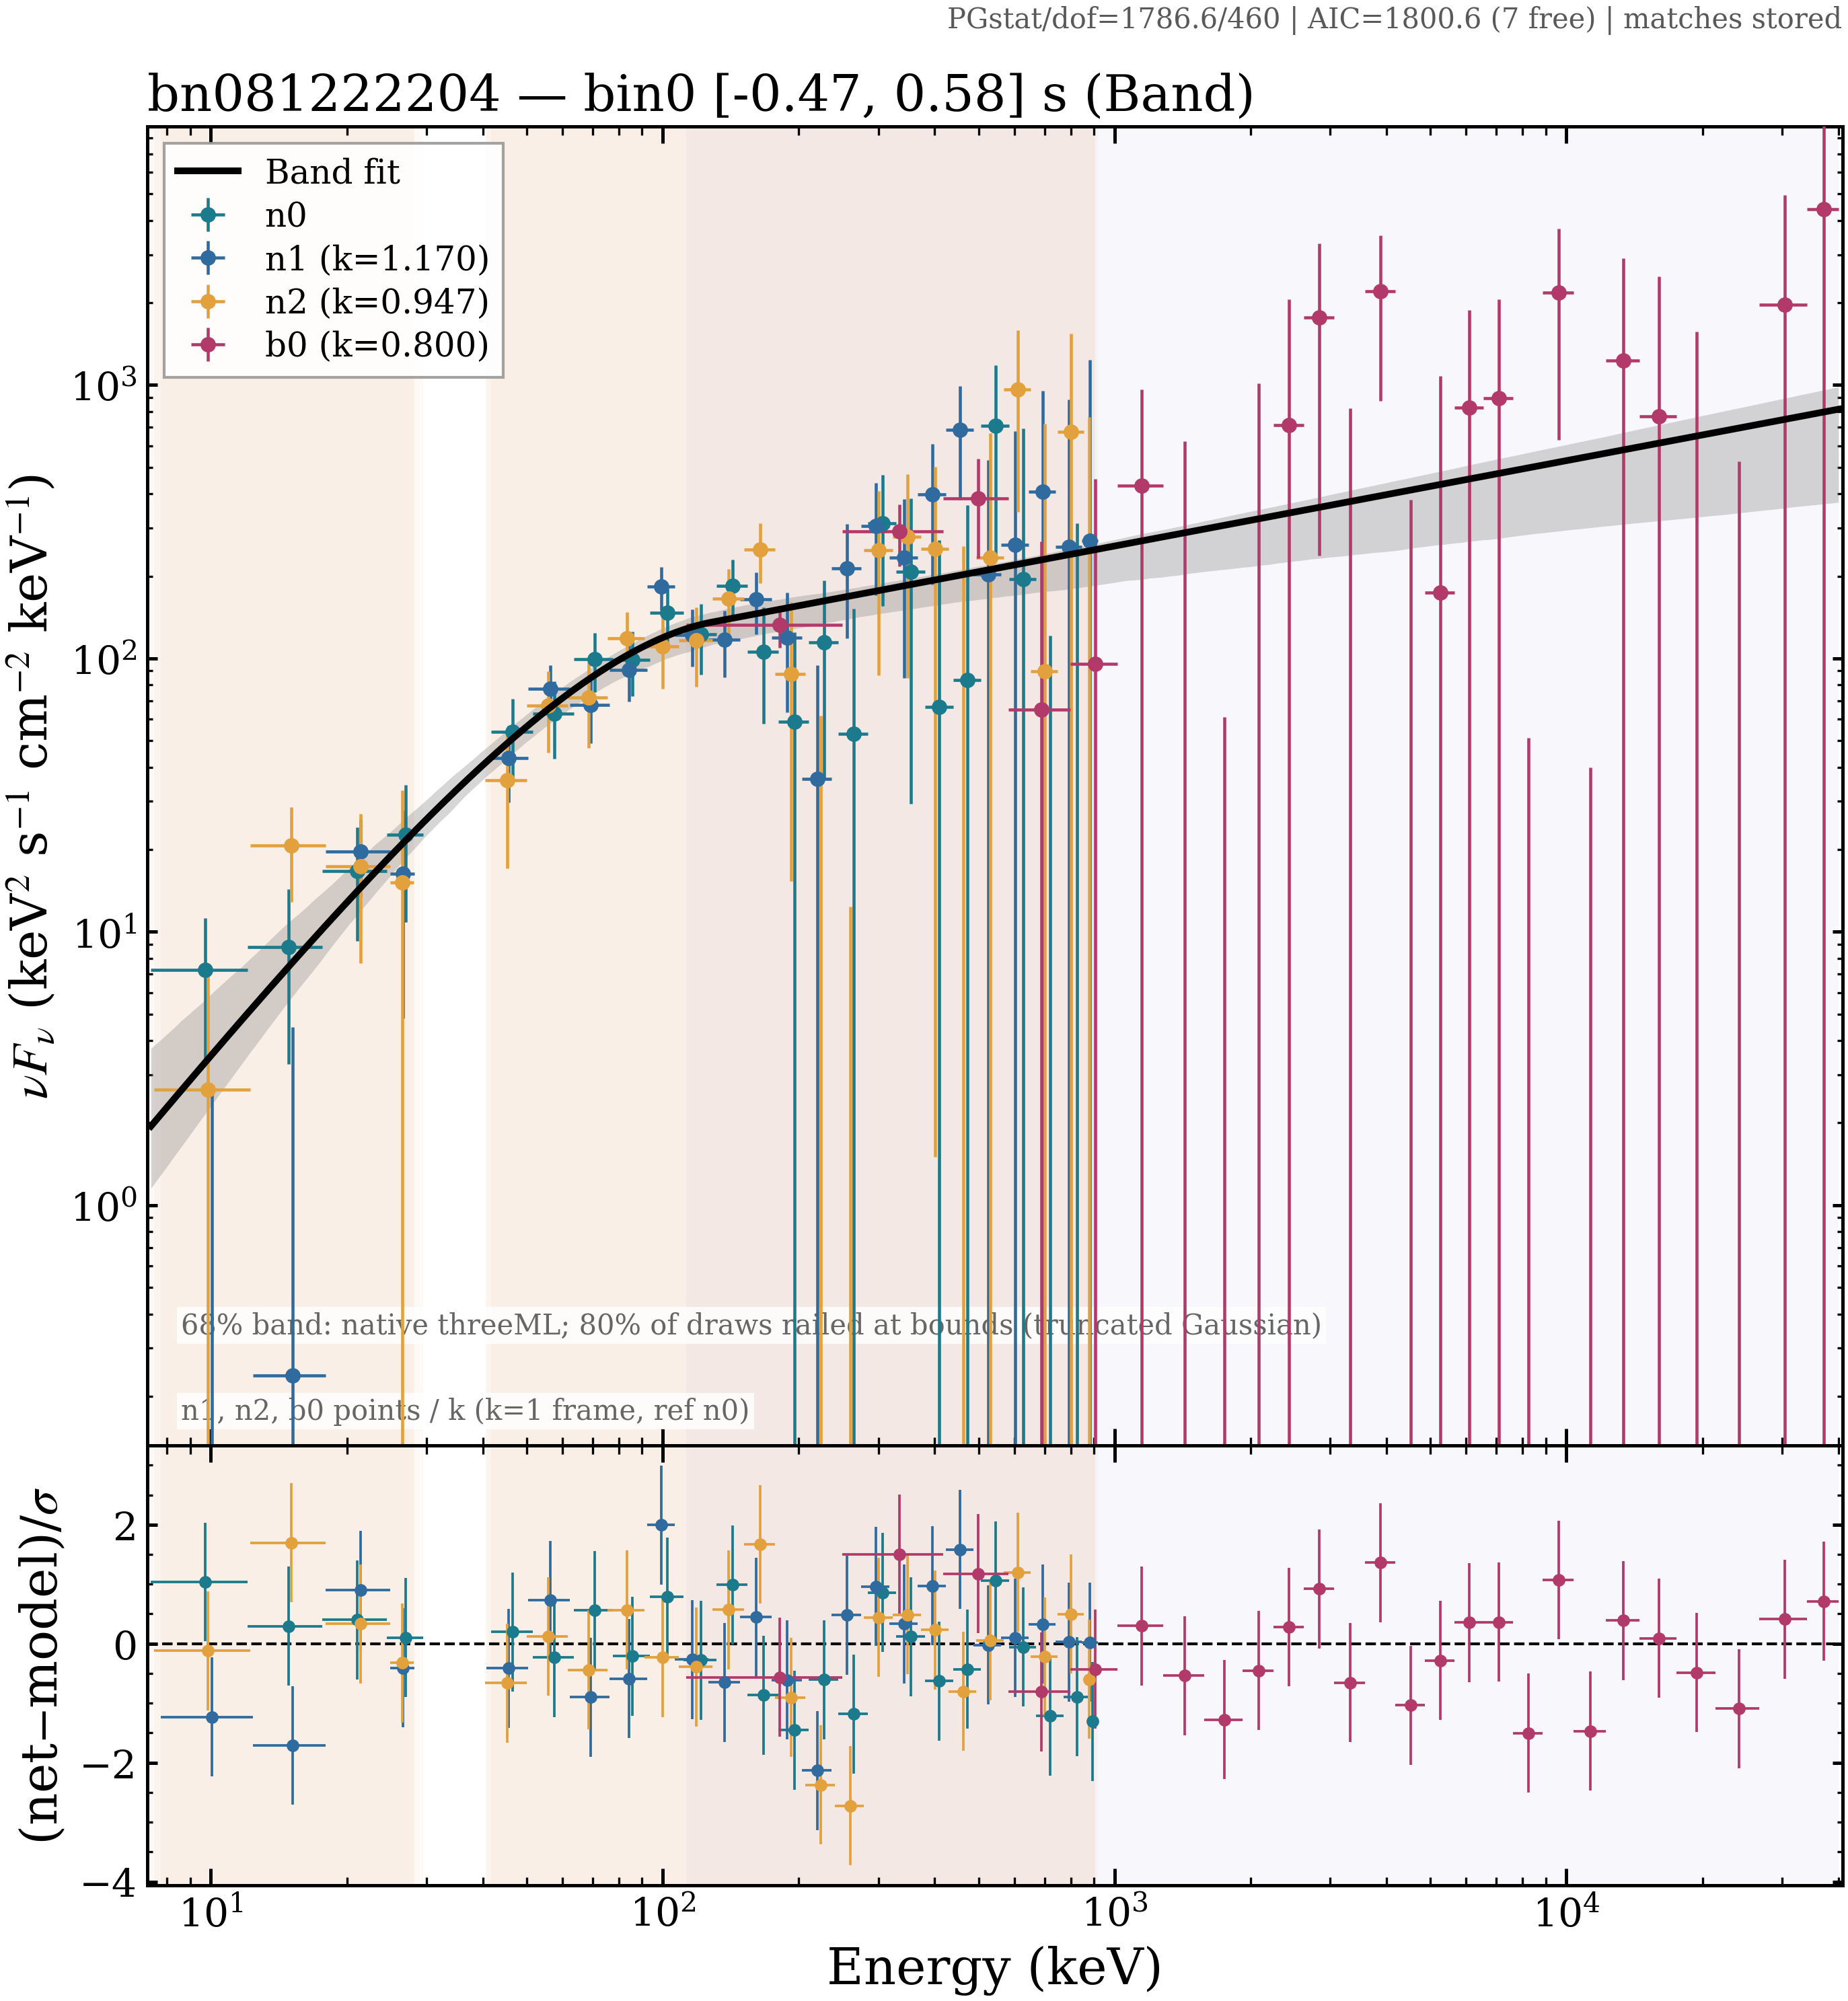
\includegraphics[width=\columnwidth]{figs/bn081222204_SED_bin0_Band.png}
\caption{The hard rise (bin 0): Band fit with $\alpha = +0.06$ and
$\beta = -1.69$ --- the tail present from the first second.
\label{fig:sedbin0}}
\end{figure}

\begin{figure}
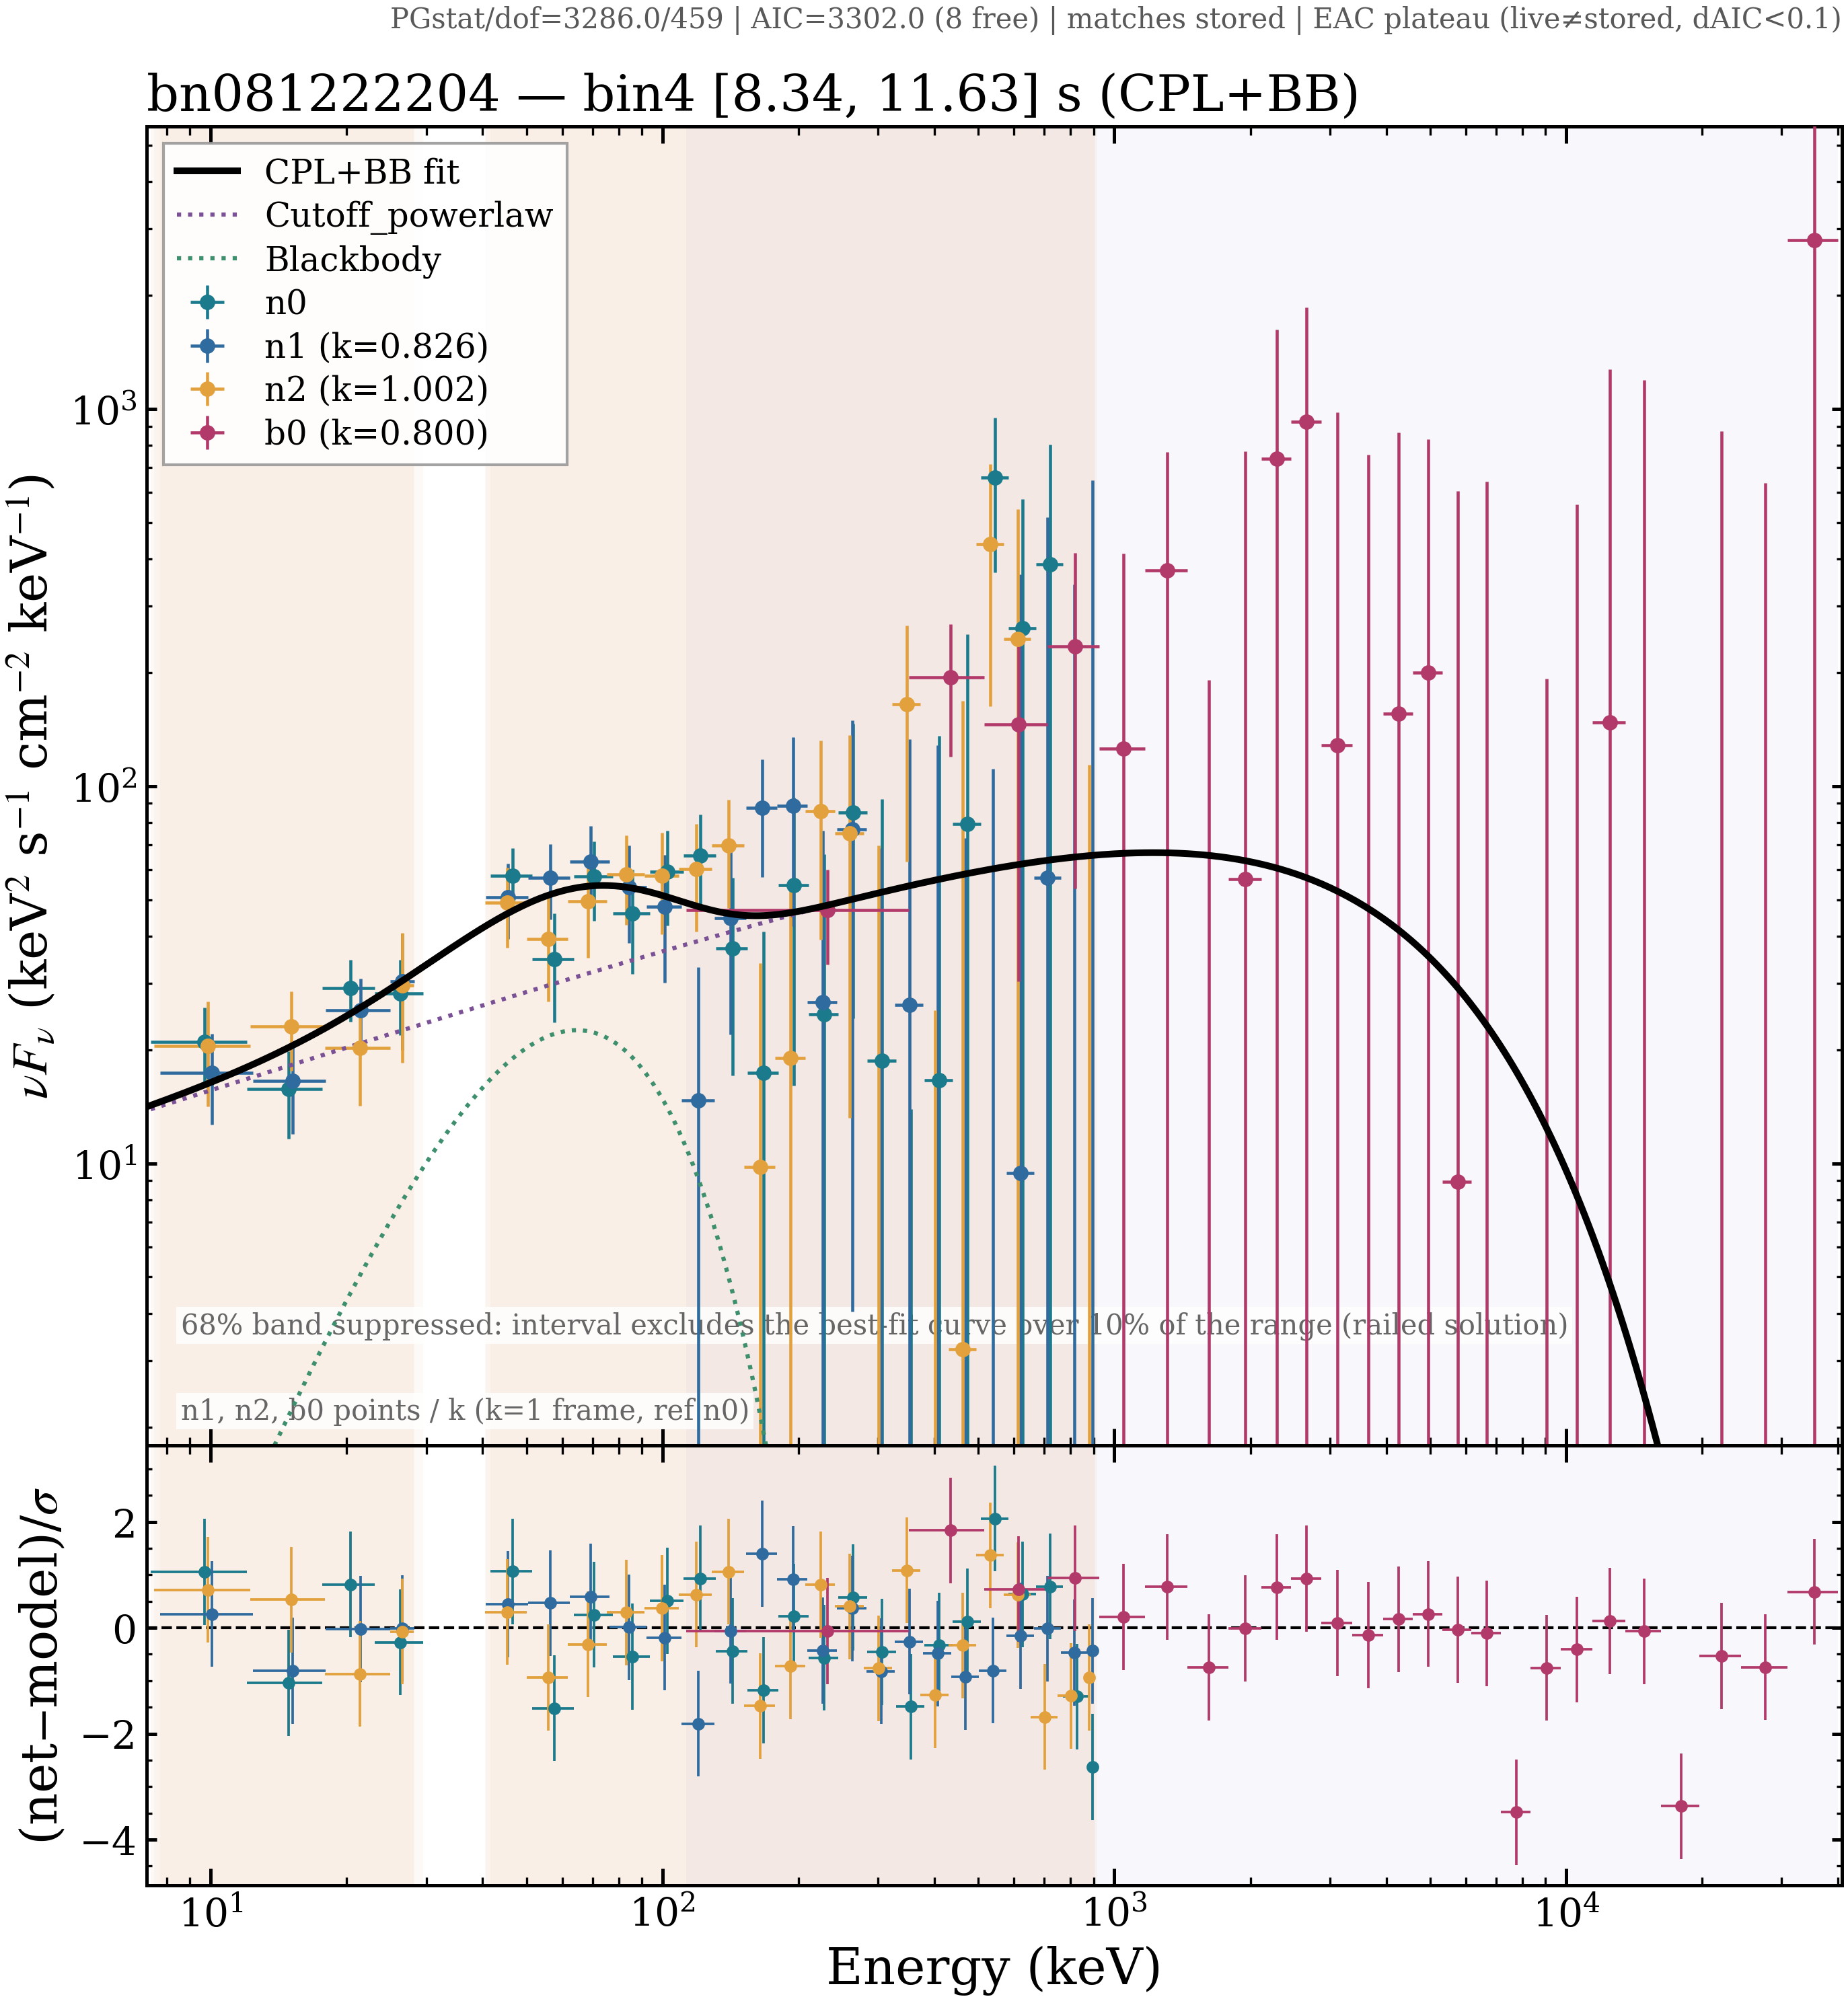
\includegraphics[width=\columnwidth]{figs/bn081222204_SED_bin4_CPLBB.png}
\caption{The bin-4 CPL+BB candidate with XSPEC-style dotted component
decomposition: the $kT = 16.5$~keV blackbody contributes a shallow
$\sim$65~keV shoulder beneath a continuum three times higher --- the
graphic form of the ``likelihood-thin'' verdict. The 68\% band is suppressed
here because the bound-railed solution's interval fails the curve-containment
guard (stated on-figure). \label{fig:sedbin4}}
\end{figure}

\begin{figure*}
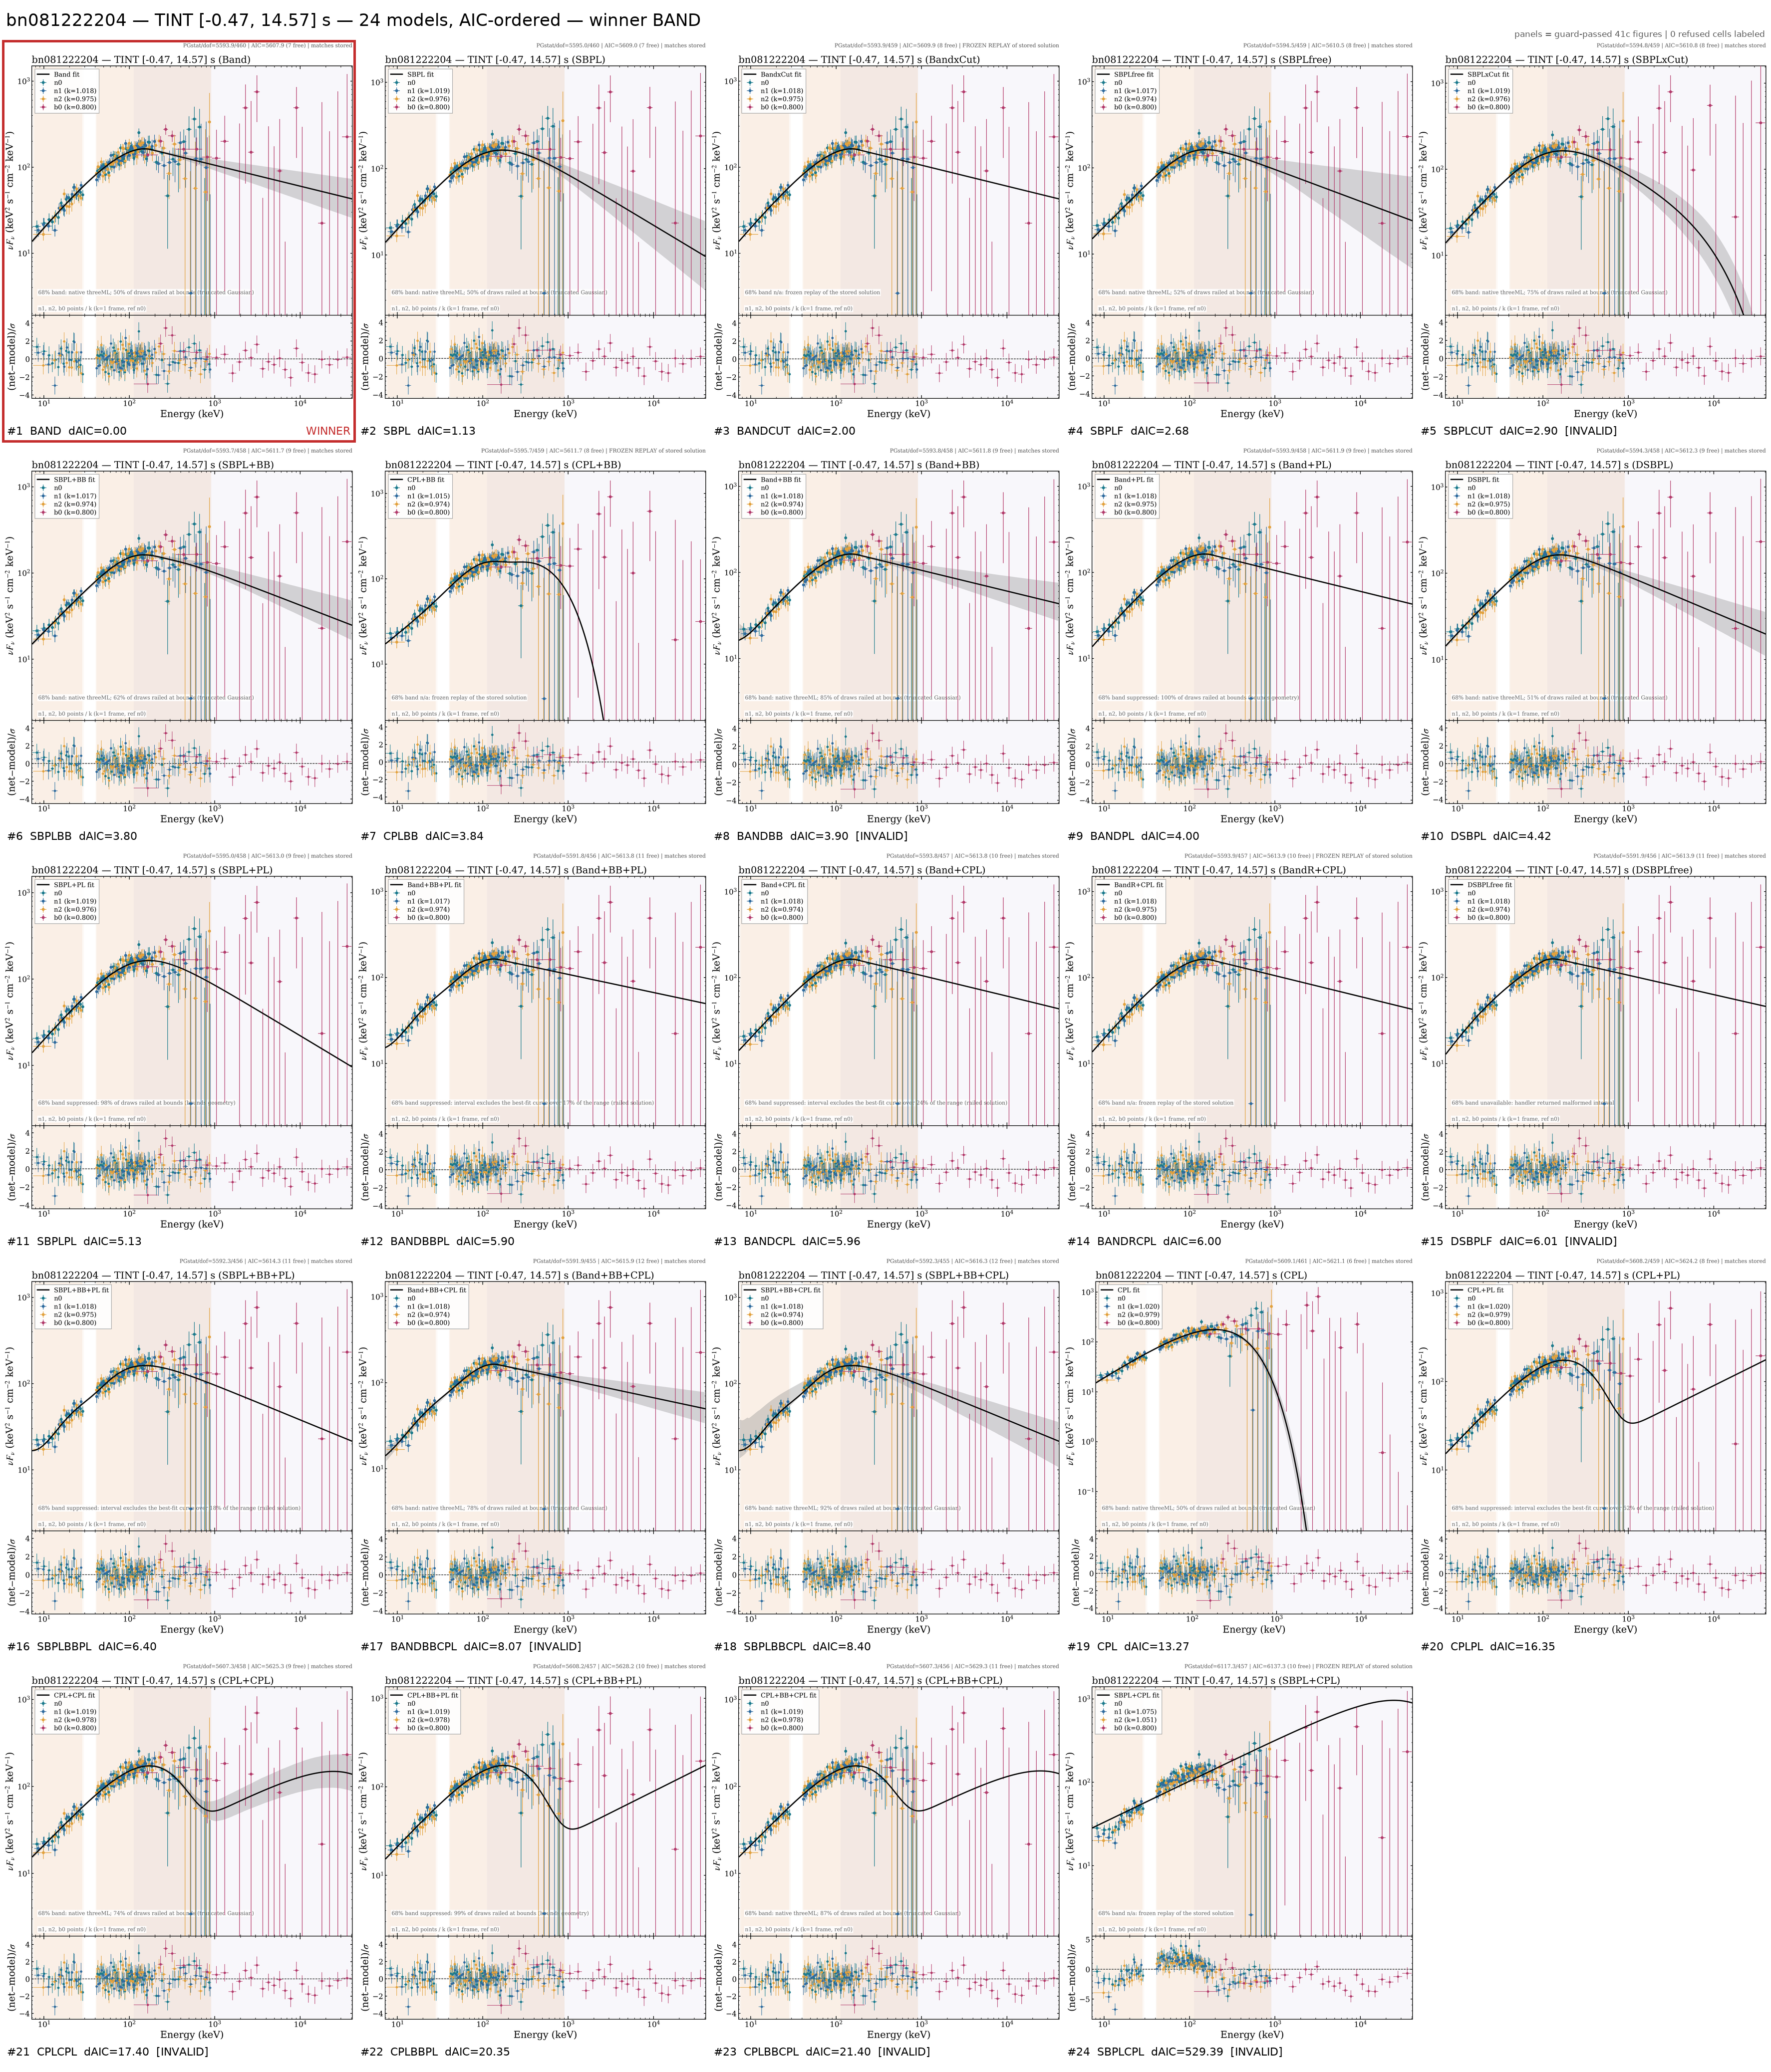
\includegraphics[width=\textwidth]{figs/bn081222204_montage_TINT.png}
\caption{All 24 models fit to the integrated spectrum, AIC-ordered (winner
framed). Every cell is a real panel under the no-model-dropped rule; frozen
replays are stamped. \label{fig:montage}}
\end{figure*}

\begin{figure}
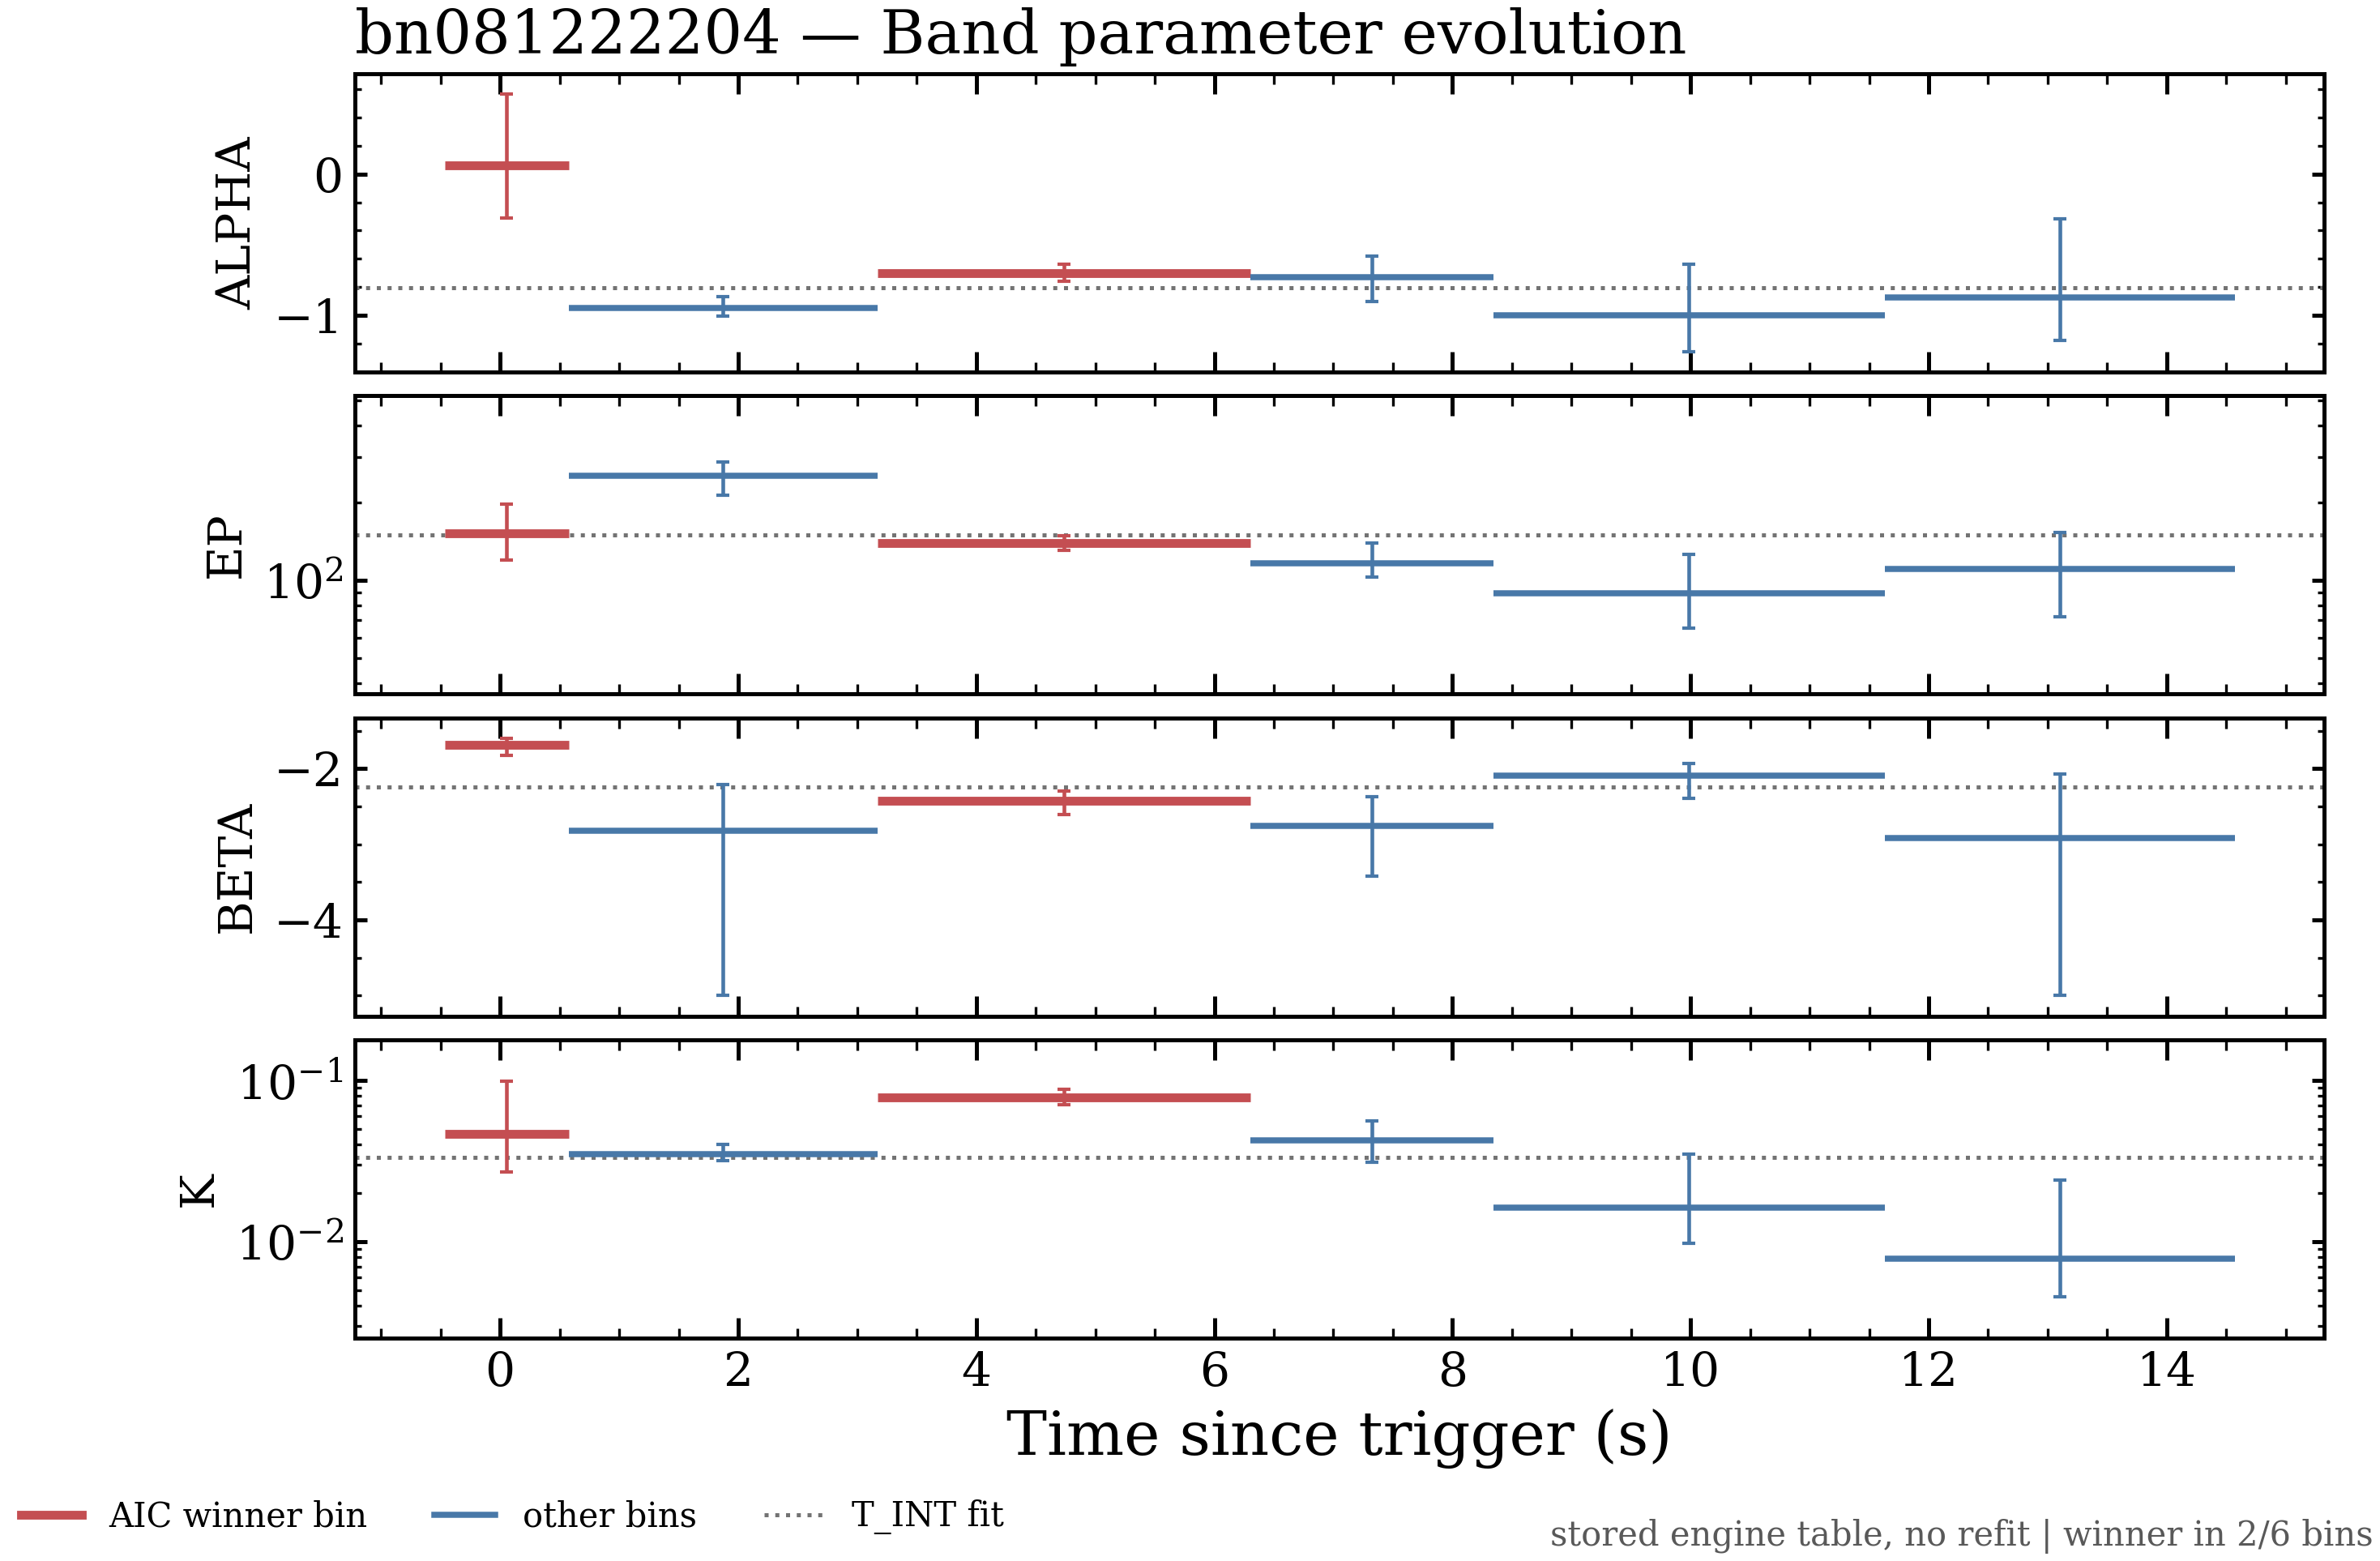
\includegraphics[width=\columnwidth]{figs/bn081222204_paramevo_BAND.png}
\caption{Band parameter evolution (red = winner bins). \label{fig:evoBAND}}
\end{figure}

\begin{figure}
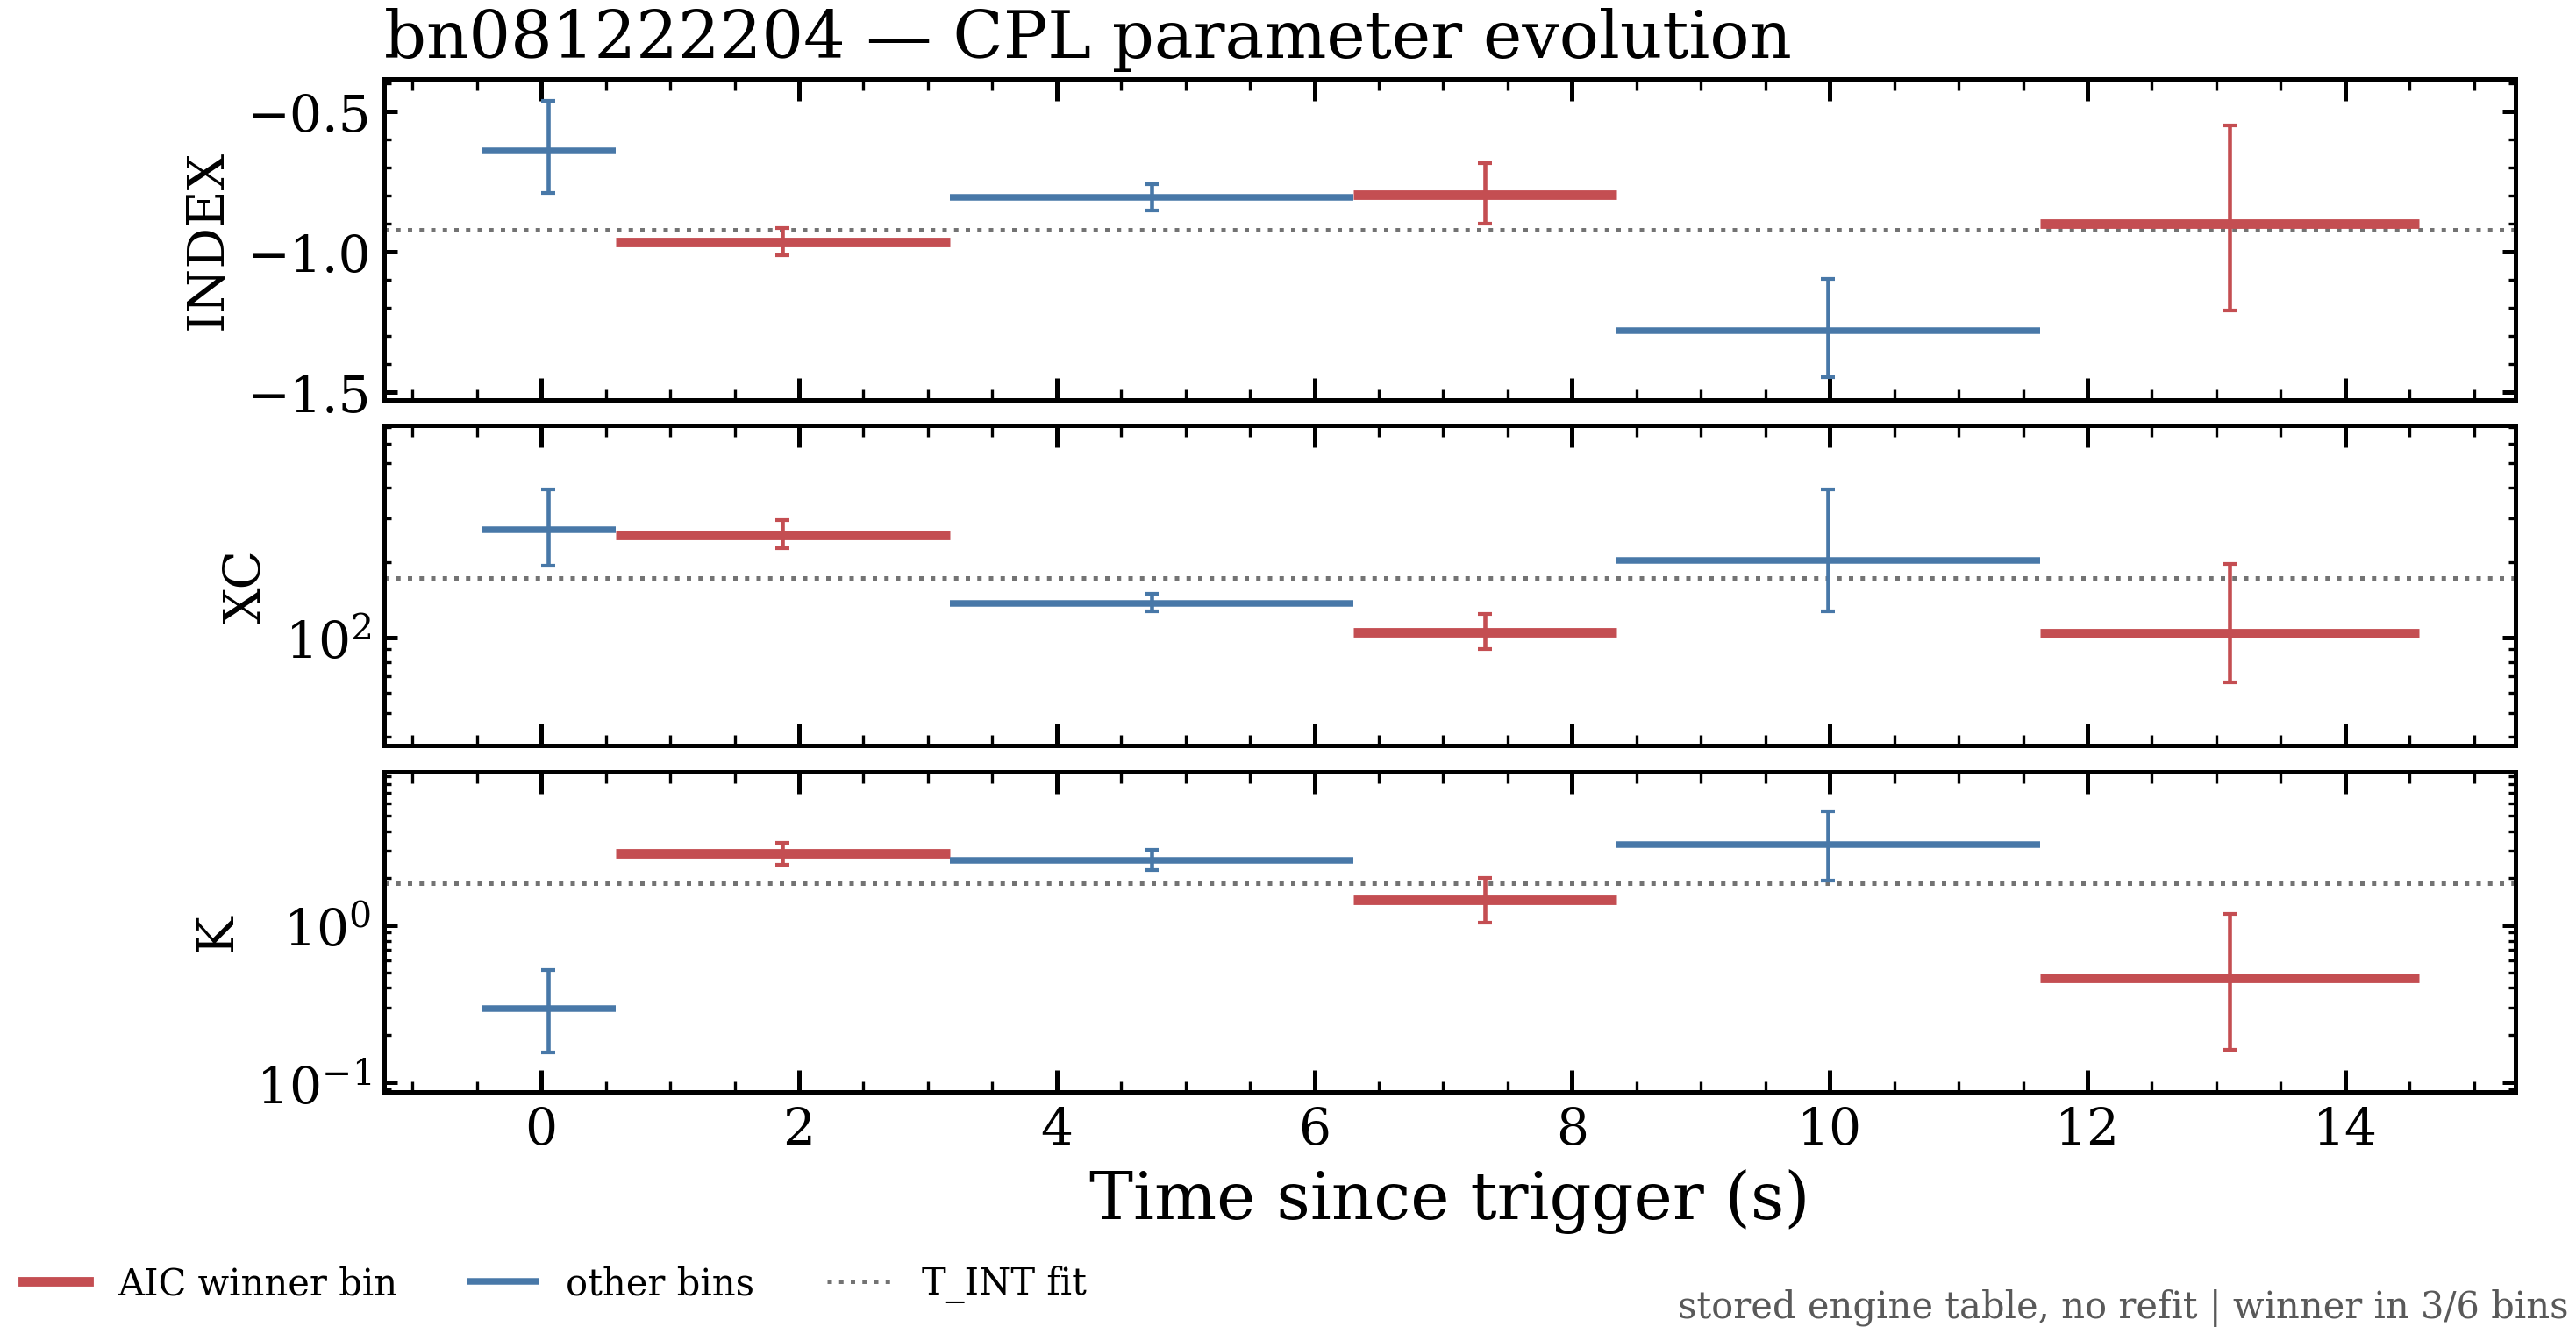
\includegraphics[width=\columnwidth]{figs/bn081222204_paramevo_CPL.png}
\caption{CPL parameter evolution: $E_{\rm c}$ decays $259 \rightarrow
104$~keV while $\Gamma$ stays near $-0.9$. \label{fig:evoCPL}}
\end{figure}

\begin{figure}
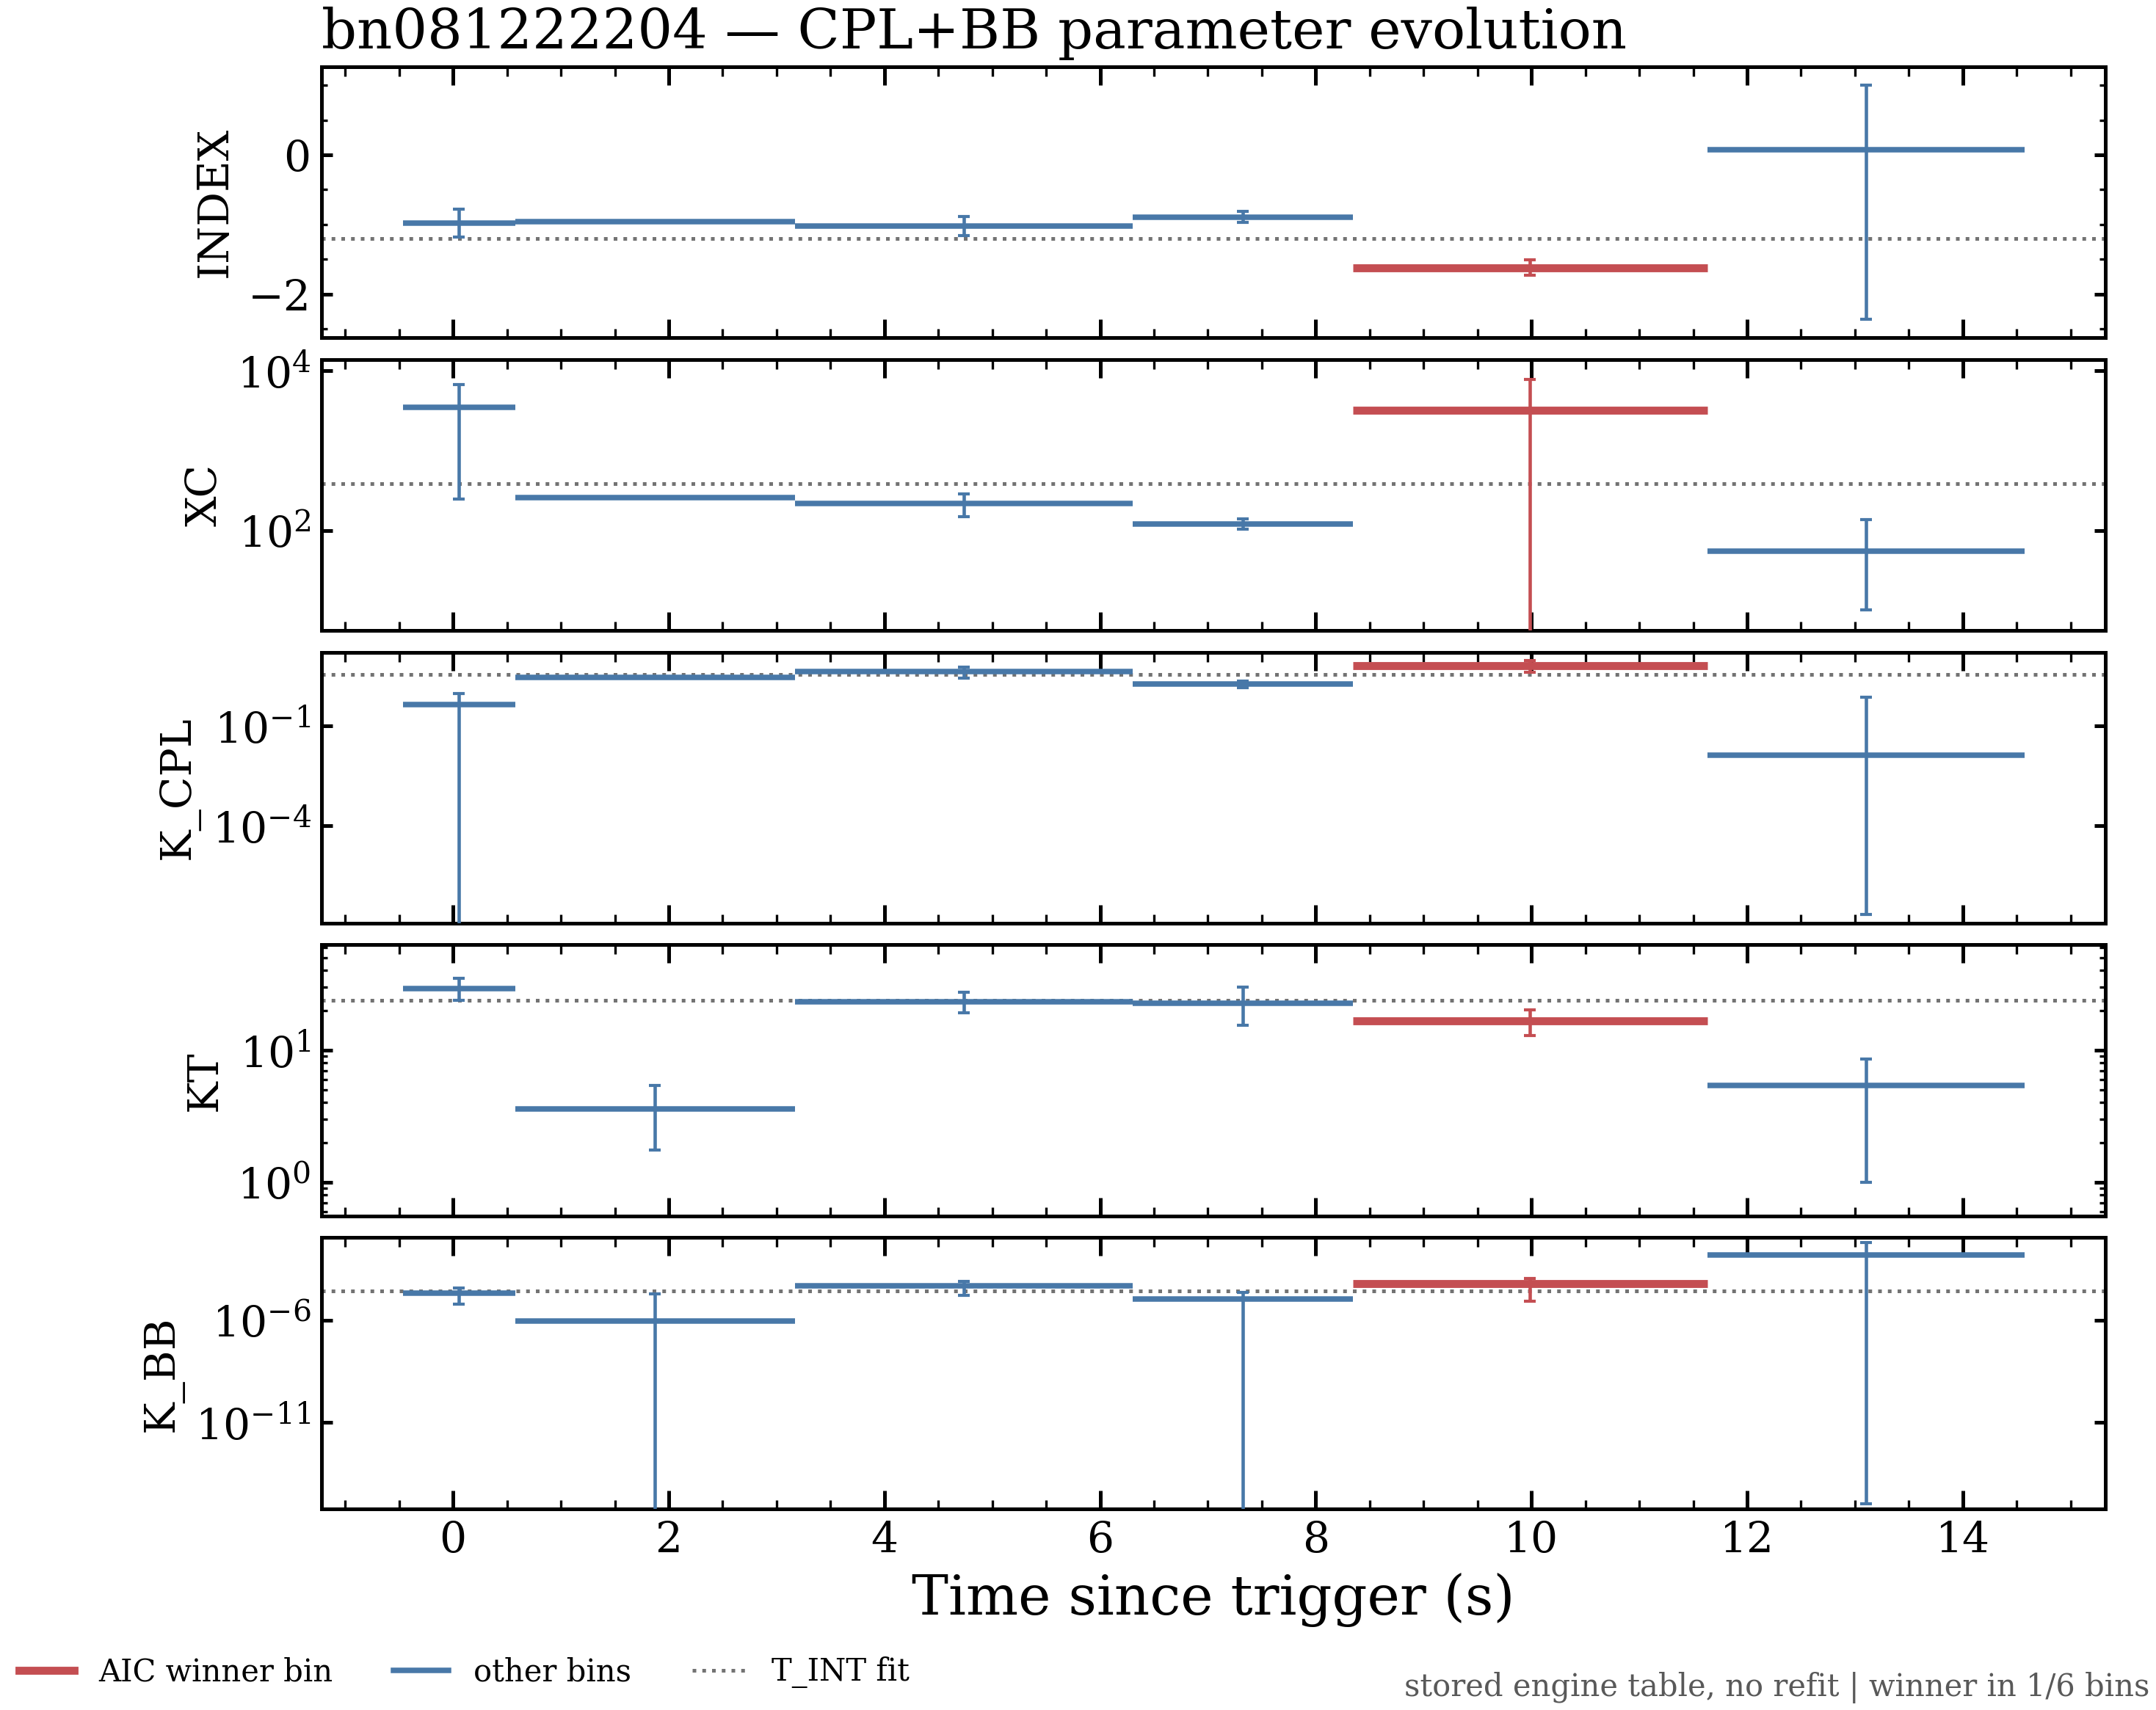
\includegraphics[width=\columnwidth]{figs/bn081222204_paramevo_CPLBB.png}
\caption{CPL+BB parameter evolution; $kT$ shows no continuity across bins
--- part of the candidate verdict. \label{fig:evoCPLBB}}
\end{figure}

\section{Discussion} \label{sec:discussion}

\textbf{Two bursts, opposite spectra.} The campaign's first two FREDs of
nearly equal asymmetry disagree on both headline spectral questions: burst
\#1 sits at $\alpha \simeq -0.3$ (violating the synchrotron line of death in
every bin) with zero thermal evidence and an integrated composite that is
evolution in disguise; \grb\ respects the limit everywhere, hosts one
physical-temperature thermal candidate, and its integrated spectrum is an
honest Band. A two-burst ``population'' proves nothing --- but it already
demonstrates that single-pulse morphology does not pin down the emission
physics, and it sets up the campaign's per-burst $\alpha$ census with a
calibration caveat attached: in both bursts one detector's effective-area
factor rails at its bound, and the burst-\#1 violation claim is gated on a
decoupling refit before it enters any census.

\textbf{The thermal question, done both ways.} Burst \#1 shows how thermal
components die at the band edge (its bin-2 ``winner'' has
$3.92\,kT < 8$~keV); \grb\ shows the opposite failure mode: a candidate that
passes the edge gate and still cannot claim detection because the residuals
do not demand it. The pair calibrates the campaign's census instrument in
both directions --- specificity and restraint.

\textbf{Timing quantities carry their estimators.} The MVT spans
$30$~ms--$1$~s on the same data depending on the question asked; the lag's
window systematic exceeds its statistical error. Rest-frame values
($T_{90} \simeq 3.0$~s, MVT $\simeq 8$~ms, $\tau \simeq 0.13$~s) enter the
campaign's lag--variability program \citep{2013ApJ...778....3S,
2025JARNA..11...27G} with those labels attached --- and the already-diverging
lag--width ratios of the first two bursts (0.085 vs.\ 0.042) preview what a
single-pulse-selected sample can say that mixed-morphology samples cannot.

\section{Analysis Provenance} \label{sec:provenance}

Every figure passed a fresh-context verification gate before inclusion
(producer--verifier separation, sha256-bound verdicts); every number binds to
a machine-readable sidecar; live display fits are hard-guarded to the stored
solutions; all 168 model panels exist under the no-model-dropped rule; the
delivery pipeline is hook-enforced (un-gated figures are mechanically
blocked). The gate ledger and per-bin reviewer notes are archived with the
campaign products; a companion paper describes the agentic pipeline.

\section{Summary} \label{sec:summary}

\begin{enumerate}
\item $T_{90} = 11.33 \pm 0.32$~s (windowed; window captures the burst;
rest frame 3.01~s); $T_{90}(E)$ follows a single power law poorly
($\chi^2/\mathrm{dof} = 4.3$); $\varphi = 0.263 \pm 0.029$ (FRED).
\item MVT $= 30.4 \pm 2.1$~ms (windowed canonical; $\approx 8$~ms rest
frame) vs.\ $215 \pm 17$~ms (global CWT, grid-quantized) and $< 1.02$~s
(Haar limit) --- estimator labels are part of the measurement.
\item Lag $= 0.474^{+0.171}_{-0.269} \pm 0.377_{\rm win}$~s: the window
systematic dominates; $\tau/T_{90} = 0.042$, half of burst \#1's ratio.
\item $\alpha = -0.70$ to $-0.96$: synchrotron-compatible throughout ---
the opposite of burst \#1; Band wins the integrated spectrum outright with
$\beta = -2.24$.
\item A physical-temperature thermal candidate ($kT = 16.5 \pm 3.7$~keV,
decay phase) passes the edge gate but fails the residual test: tracked,
not detected.
\item All 168 (model, bin) panels exist under the no-model-dropped rule;
every figure and number carries verified provenance.
\end{enumerate}

\begin{acknowledgments}
\textit{Fermi}/GBM public data; analysis with 3ML
\citep{2015arXiv150708343V}. Produced by the single-pulse campaign's staged,
gate-reviewed agentic pipeline; all numbers provisional pending the campaign
freeze.
\end{acknowledgments}

\appendix

\section{Per-bin model montages} \label{app:montages}

\begin{figure*}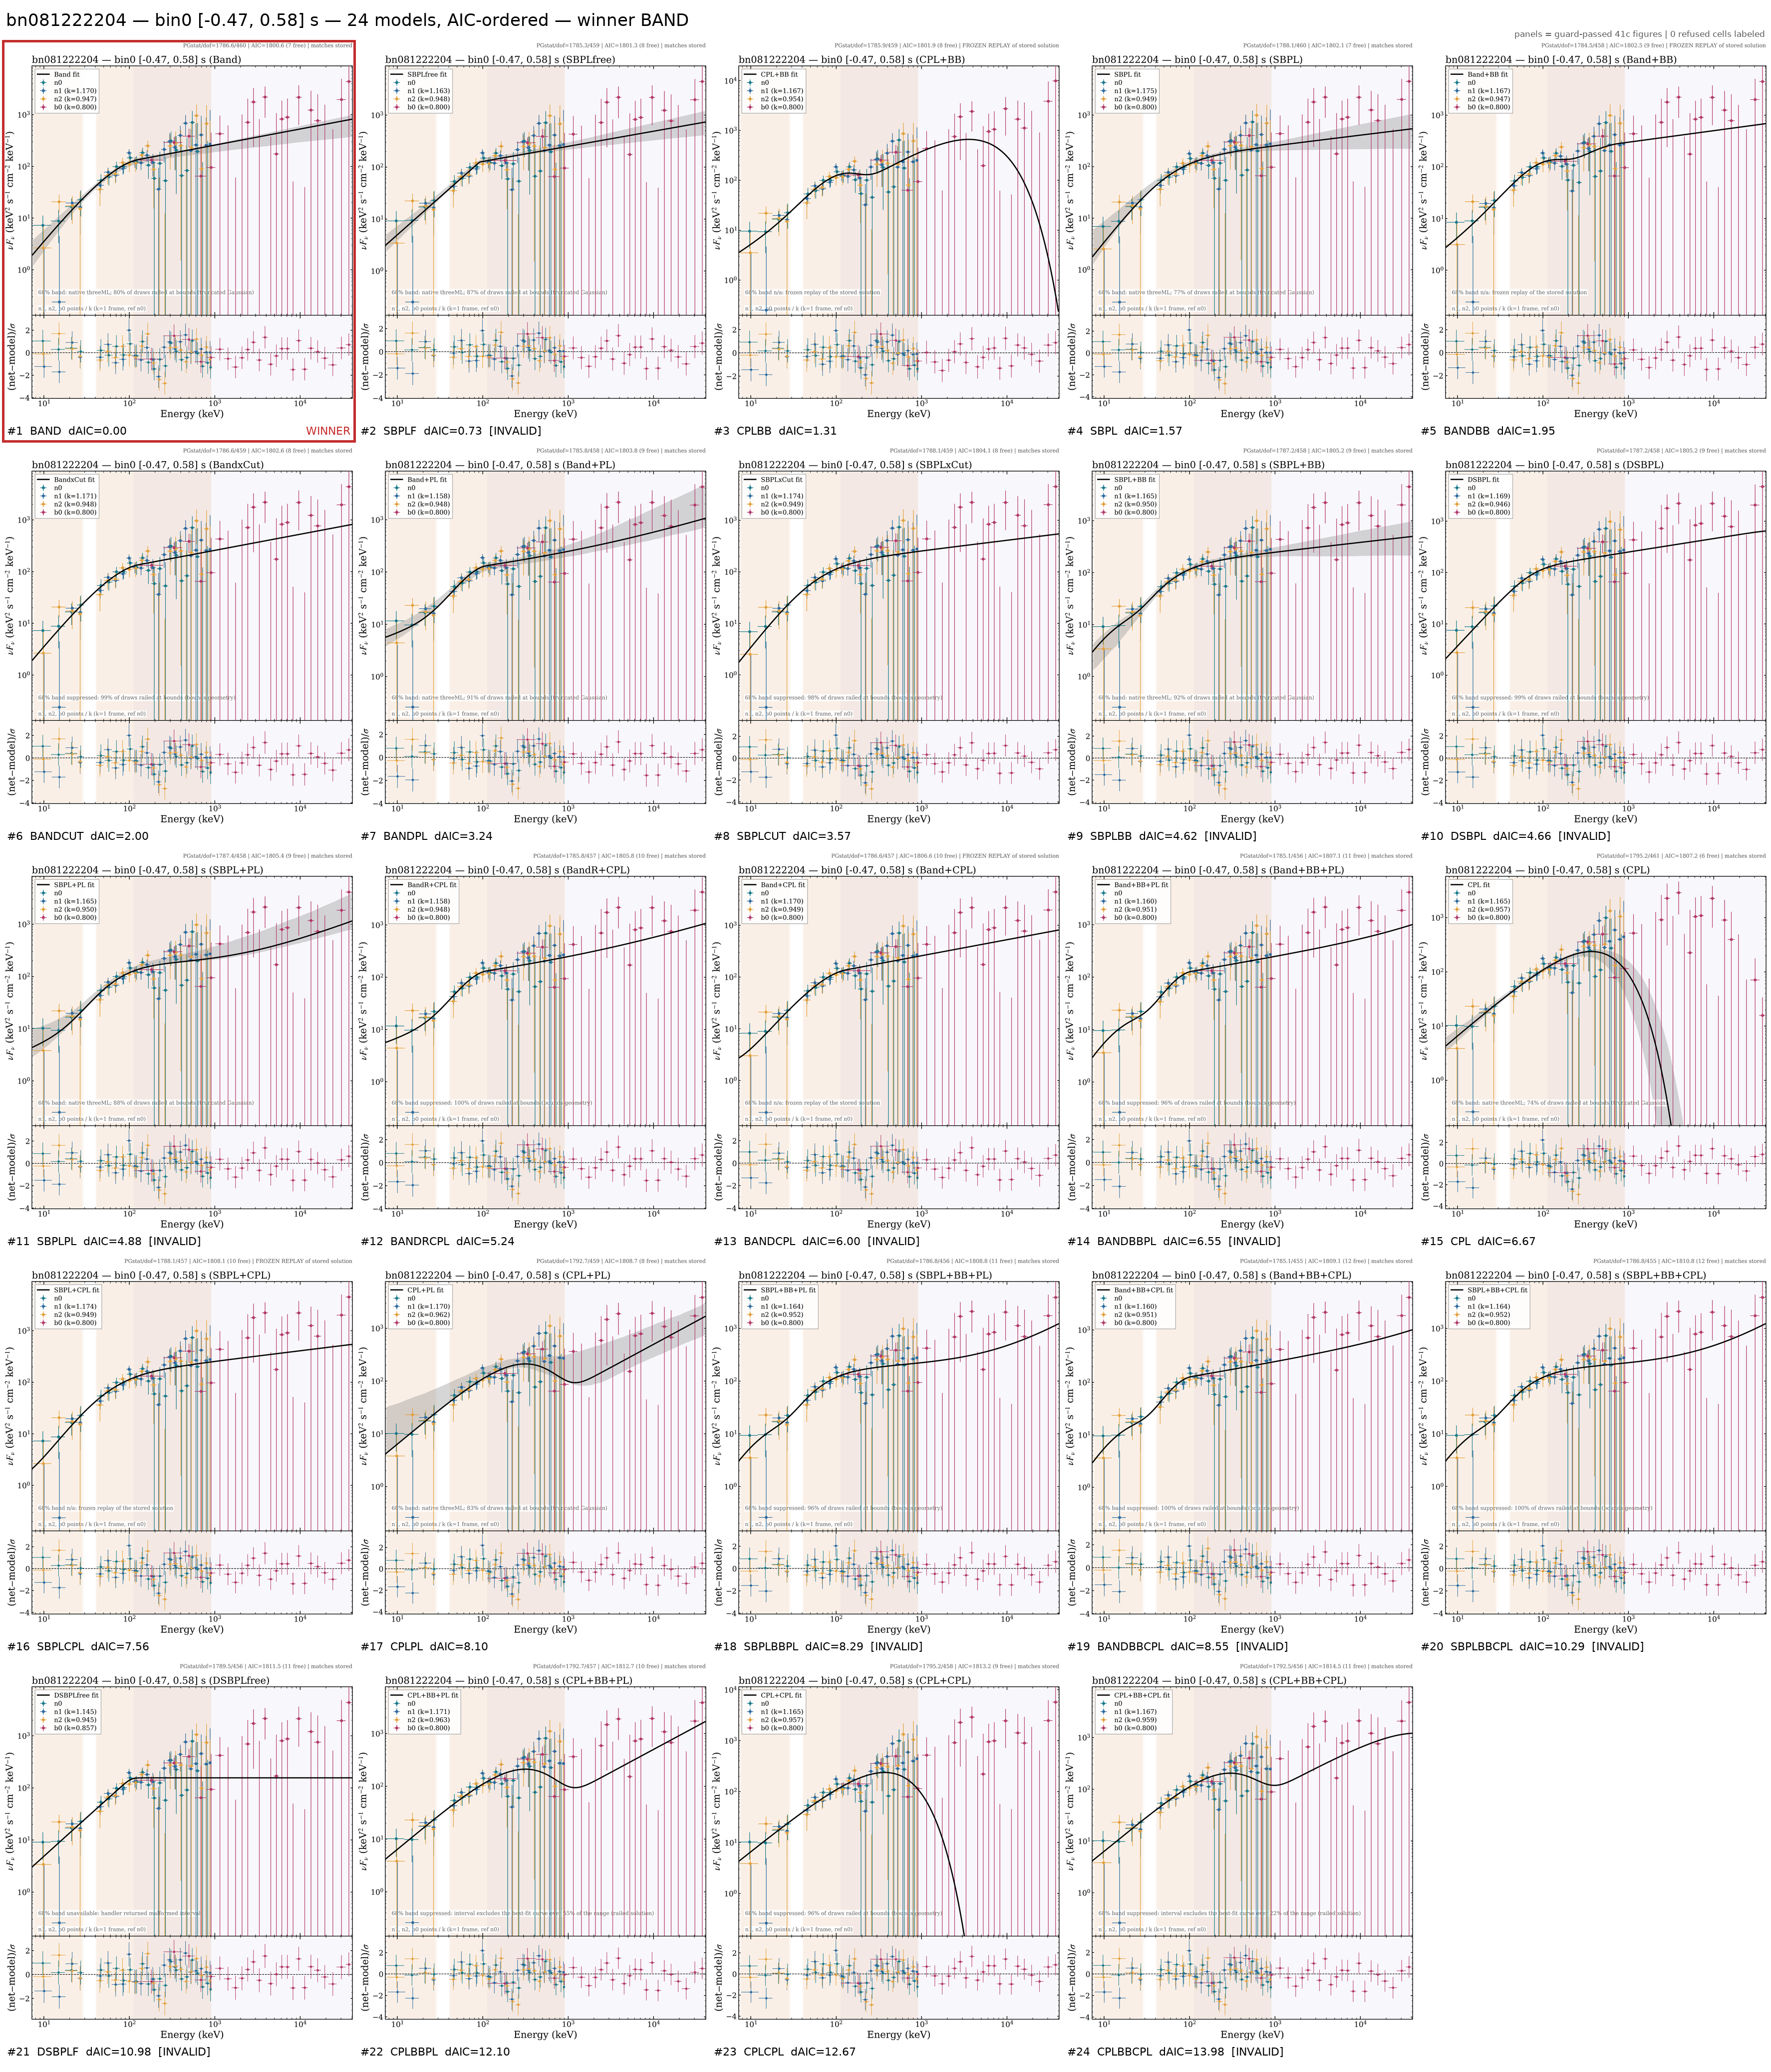
\includegraphics[width=\textwidth]{figs/bn081222204_montage_bin0.png}
\caption{Bin 0 montage.}\end{figure*}
\begin{figure*}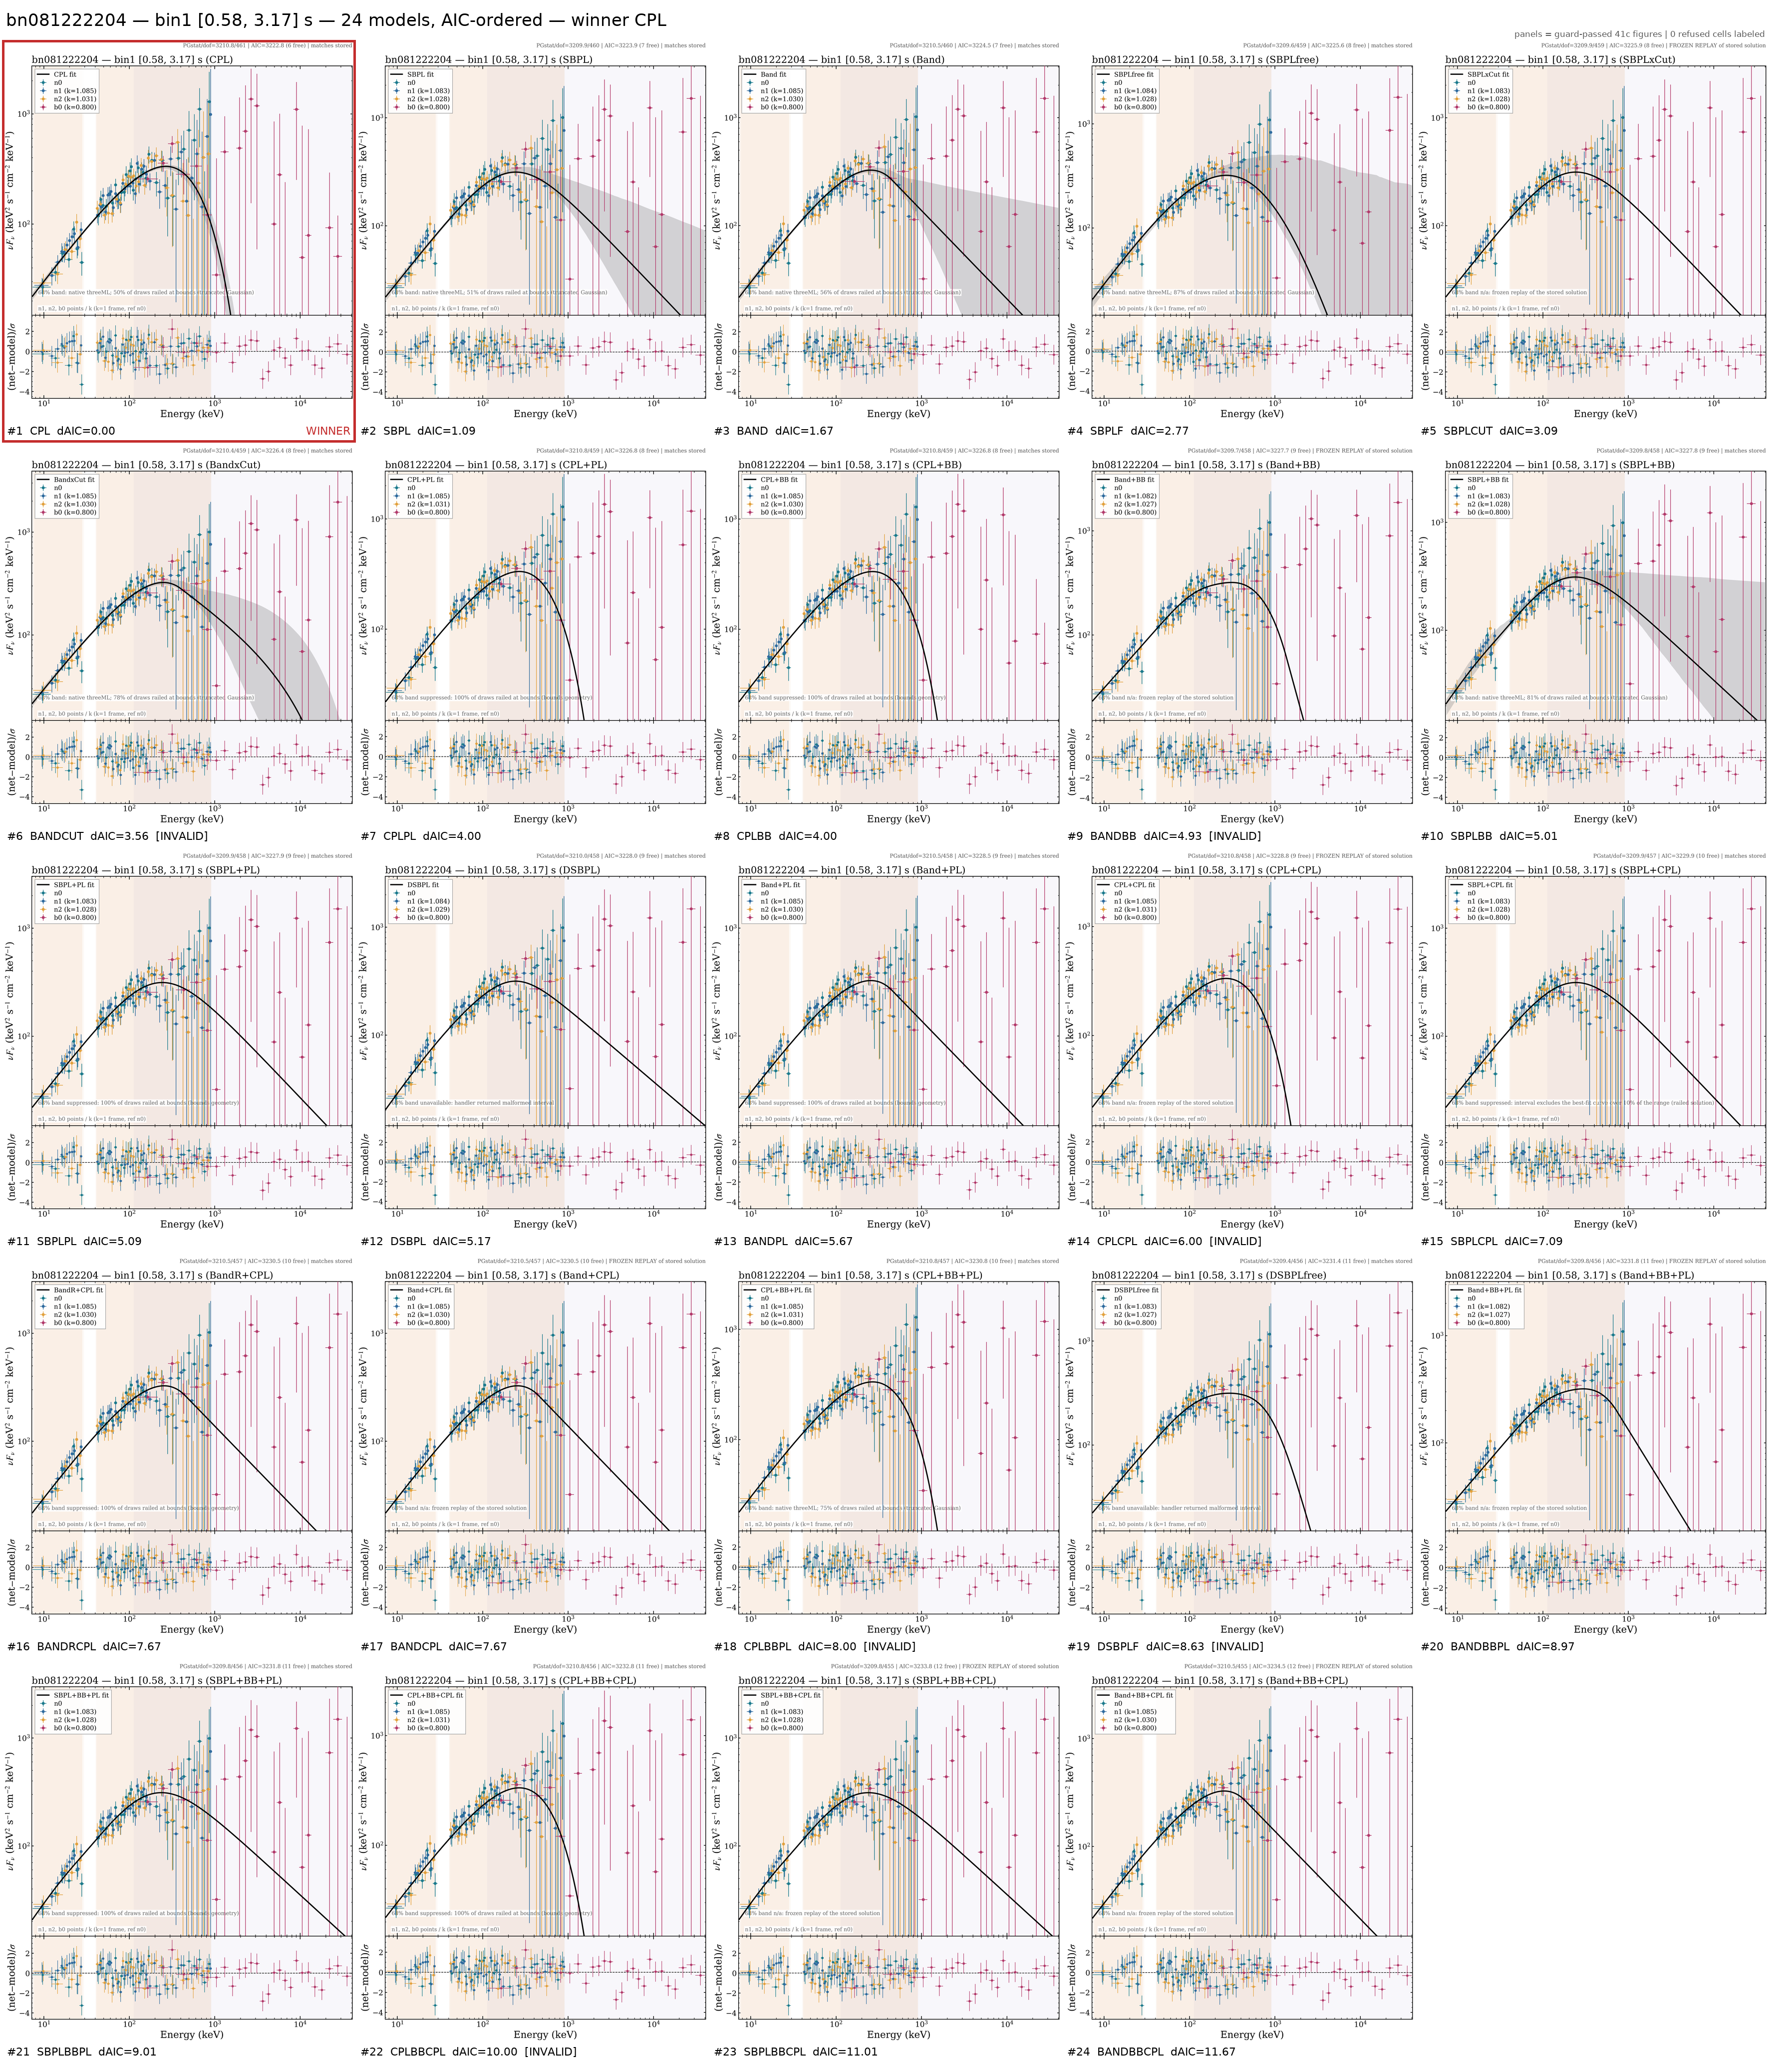
\includegraphics[width=\textwidth]{figs/bn081222204_montage_bin1.png}
\caption{Bin 1 montage.}\end{figure*}
\begin{figure*}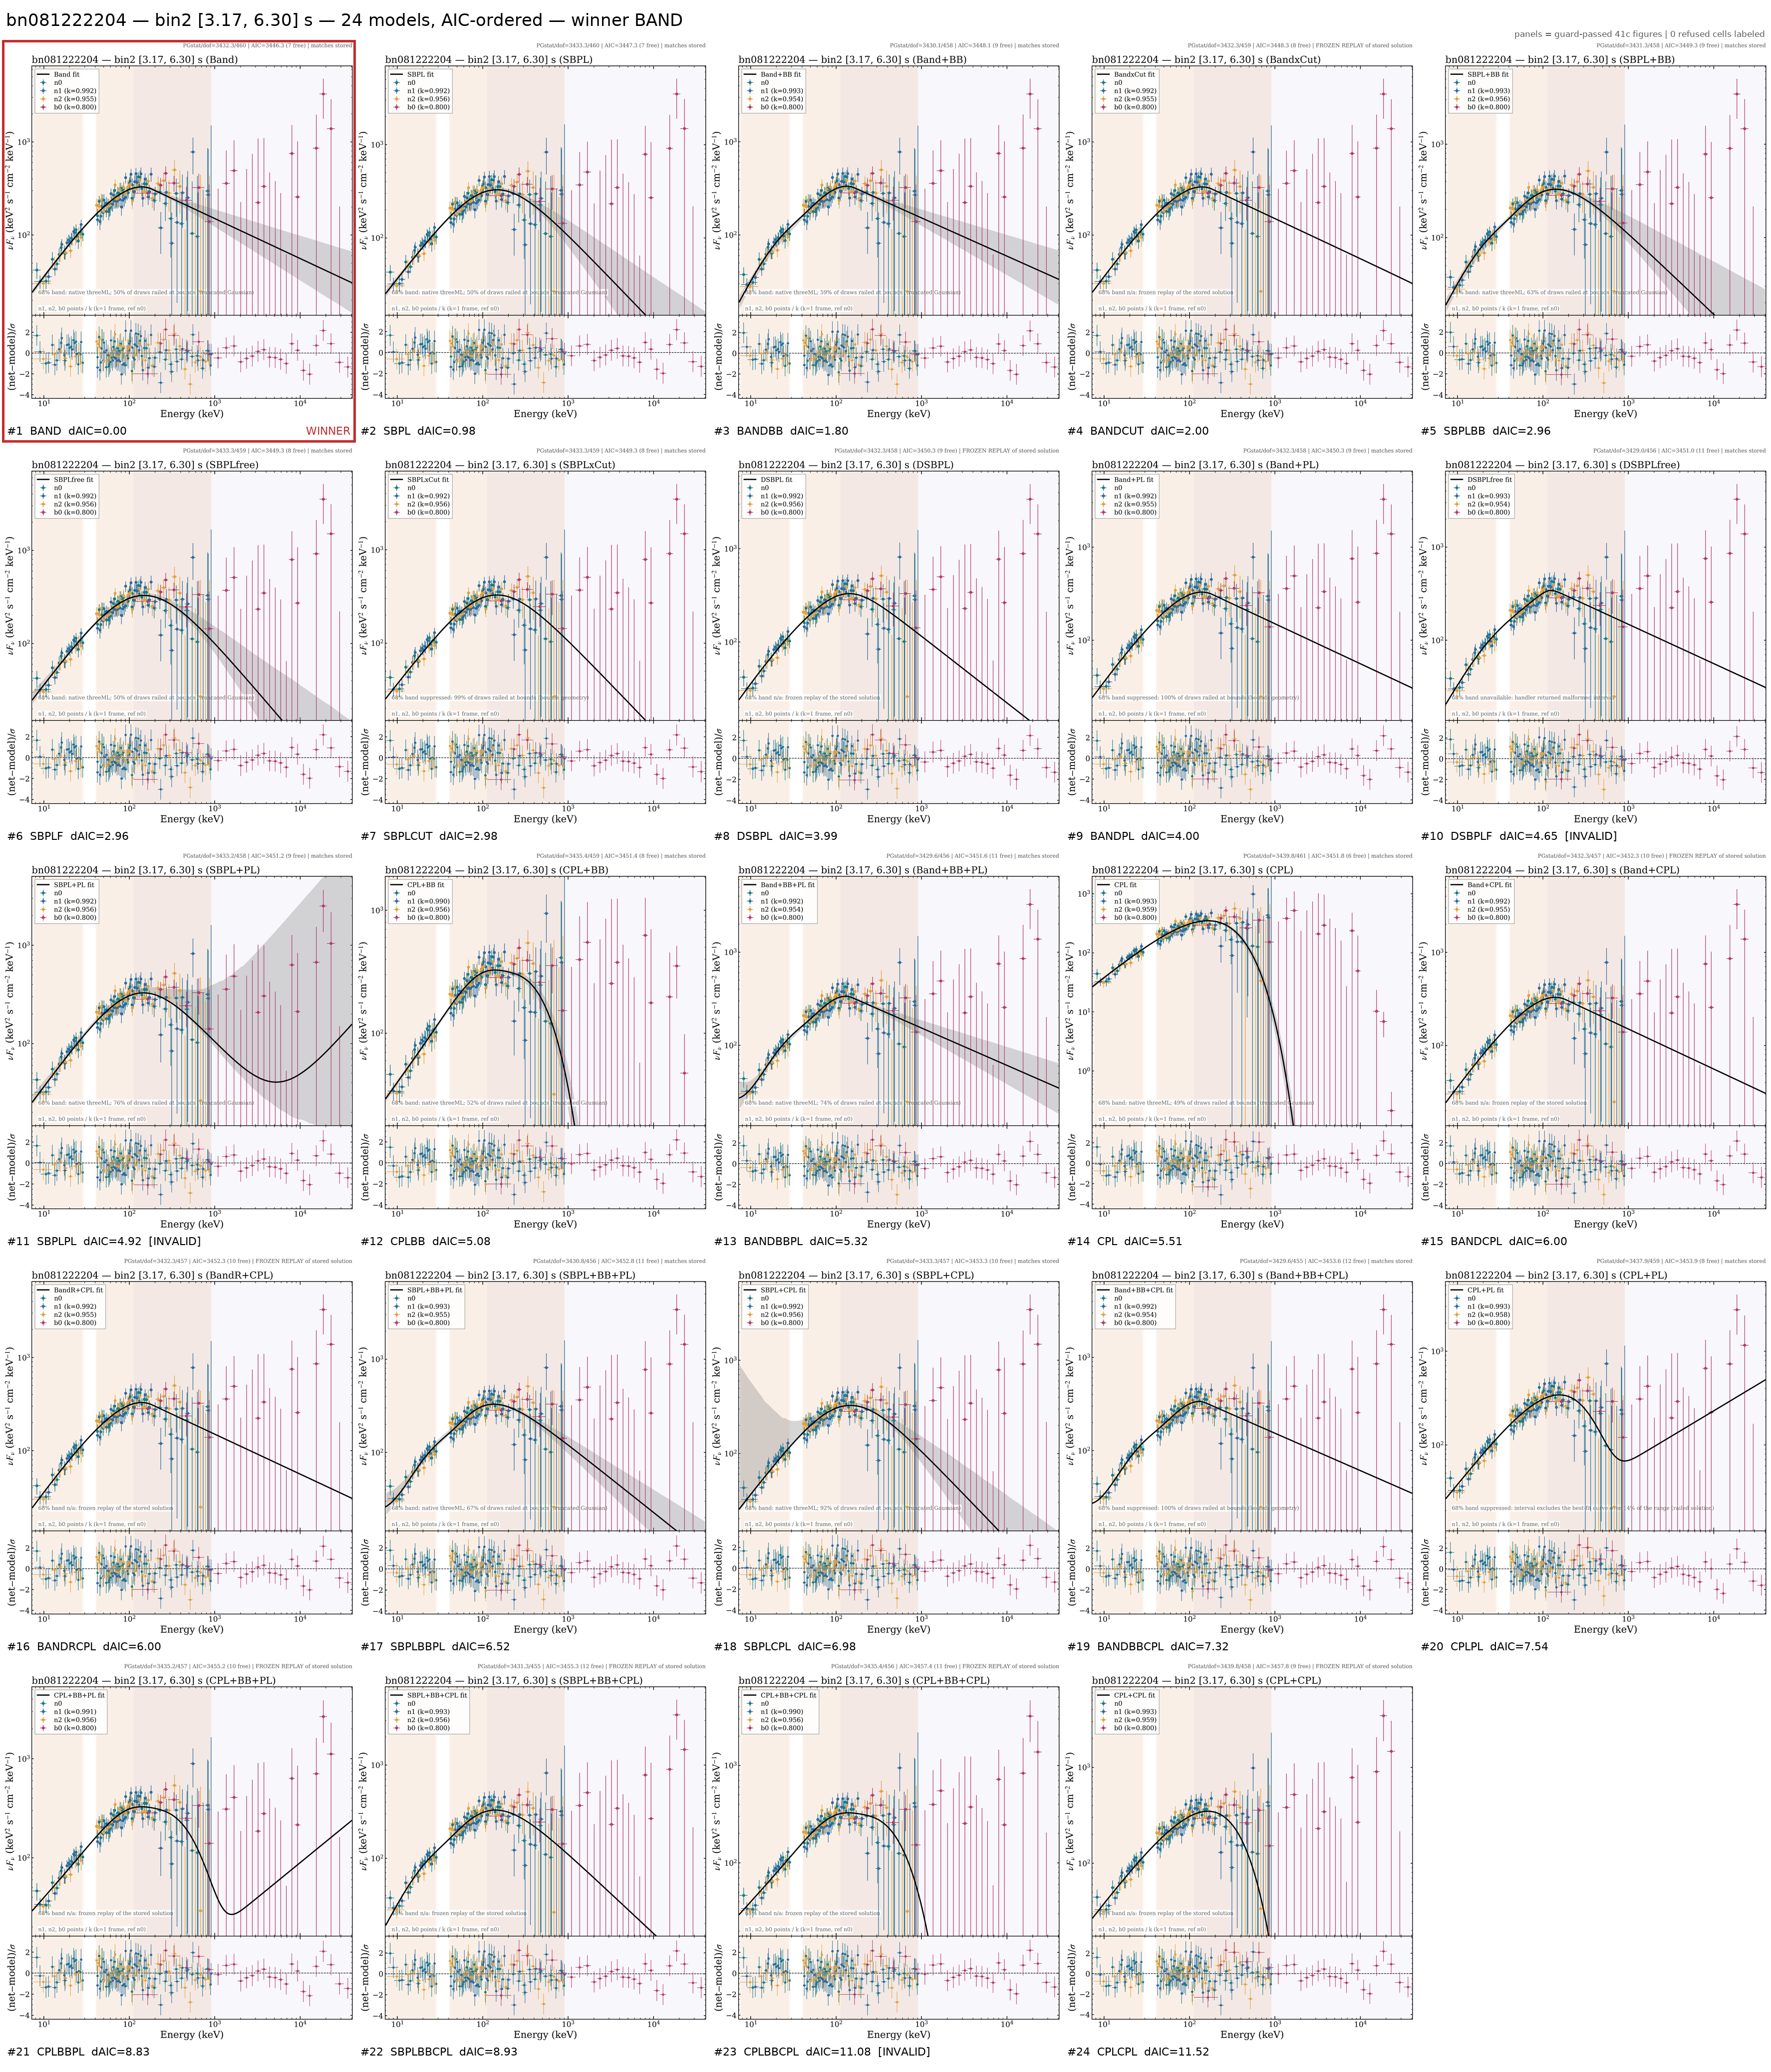
\includegraphics[width=\textwidth]{figs/bn081222204_montage_bin2.png}
\caption{Bin 2 montage.}\end{figure*}
\begin{figure*}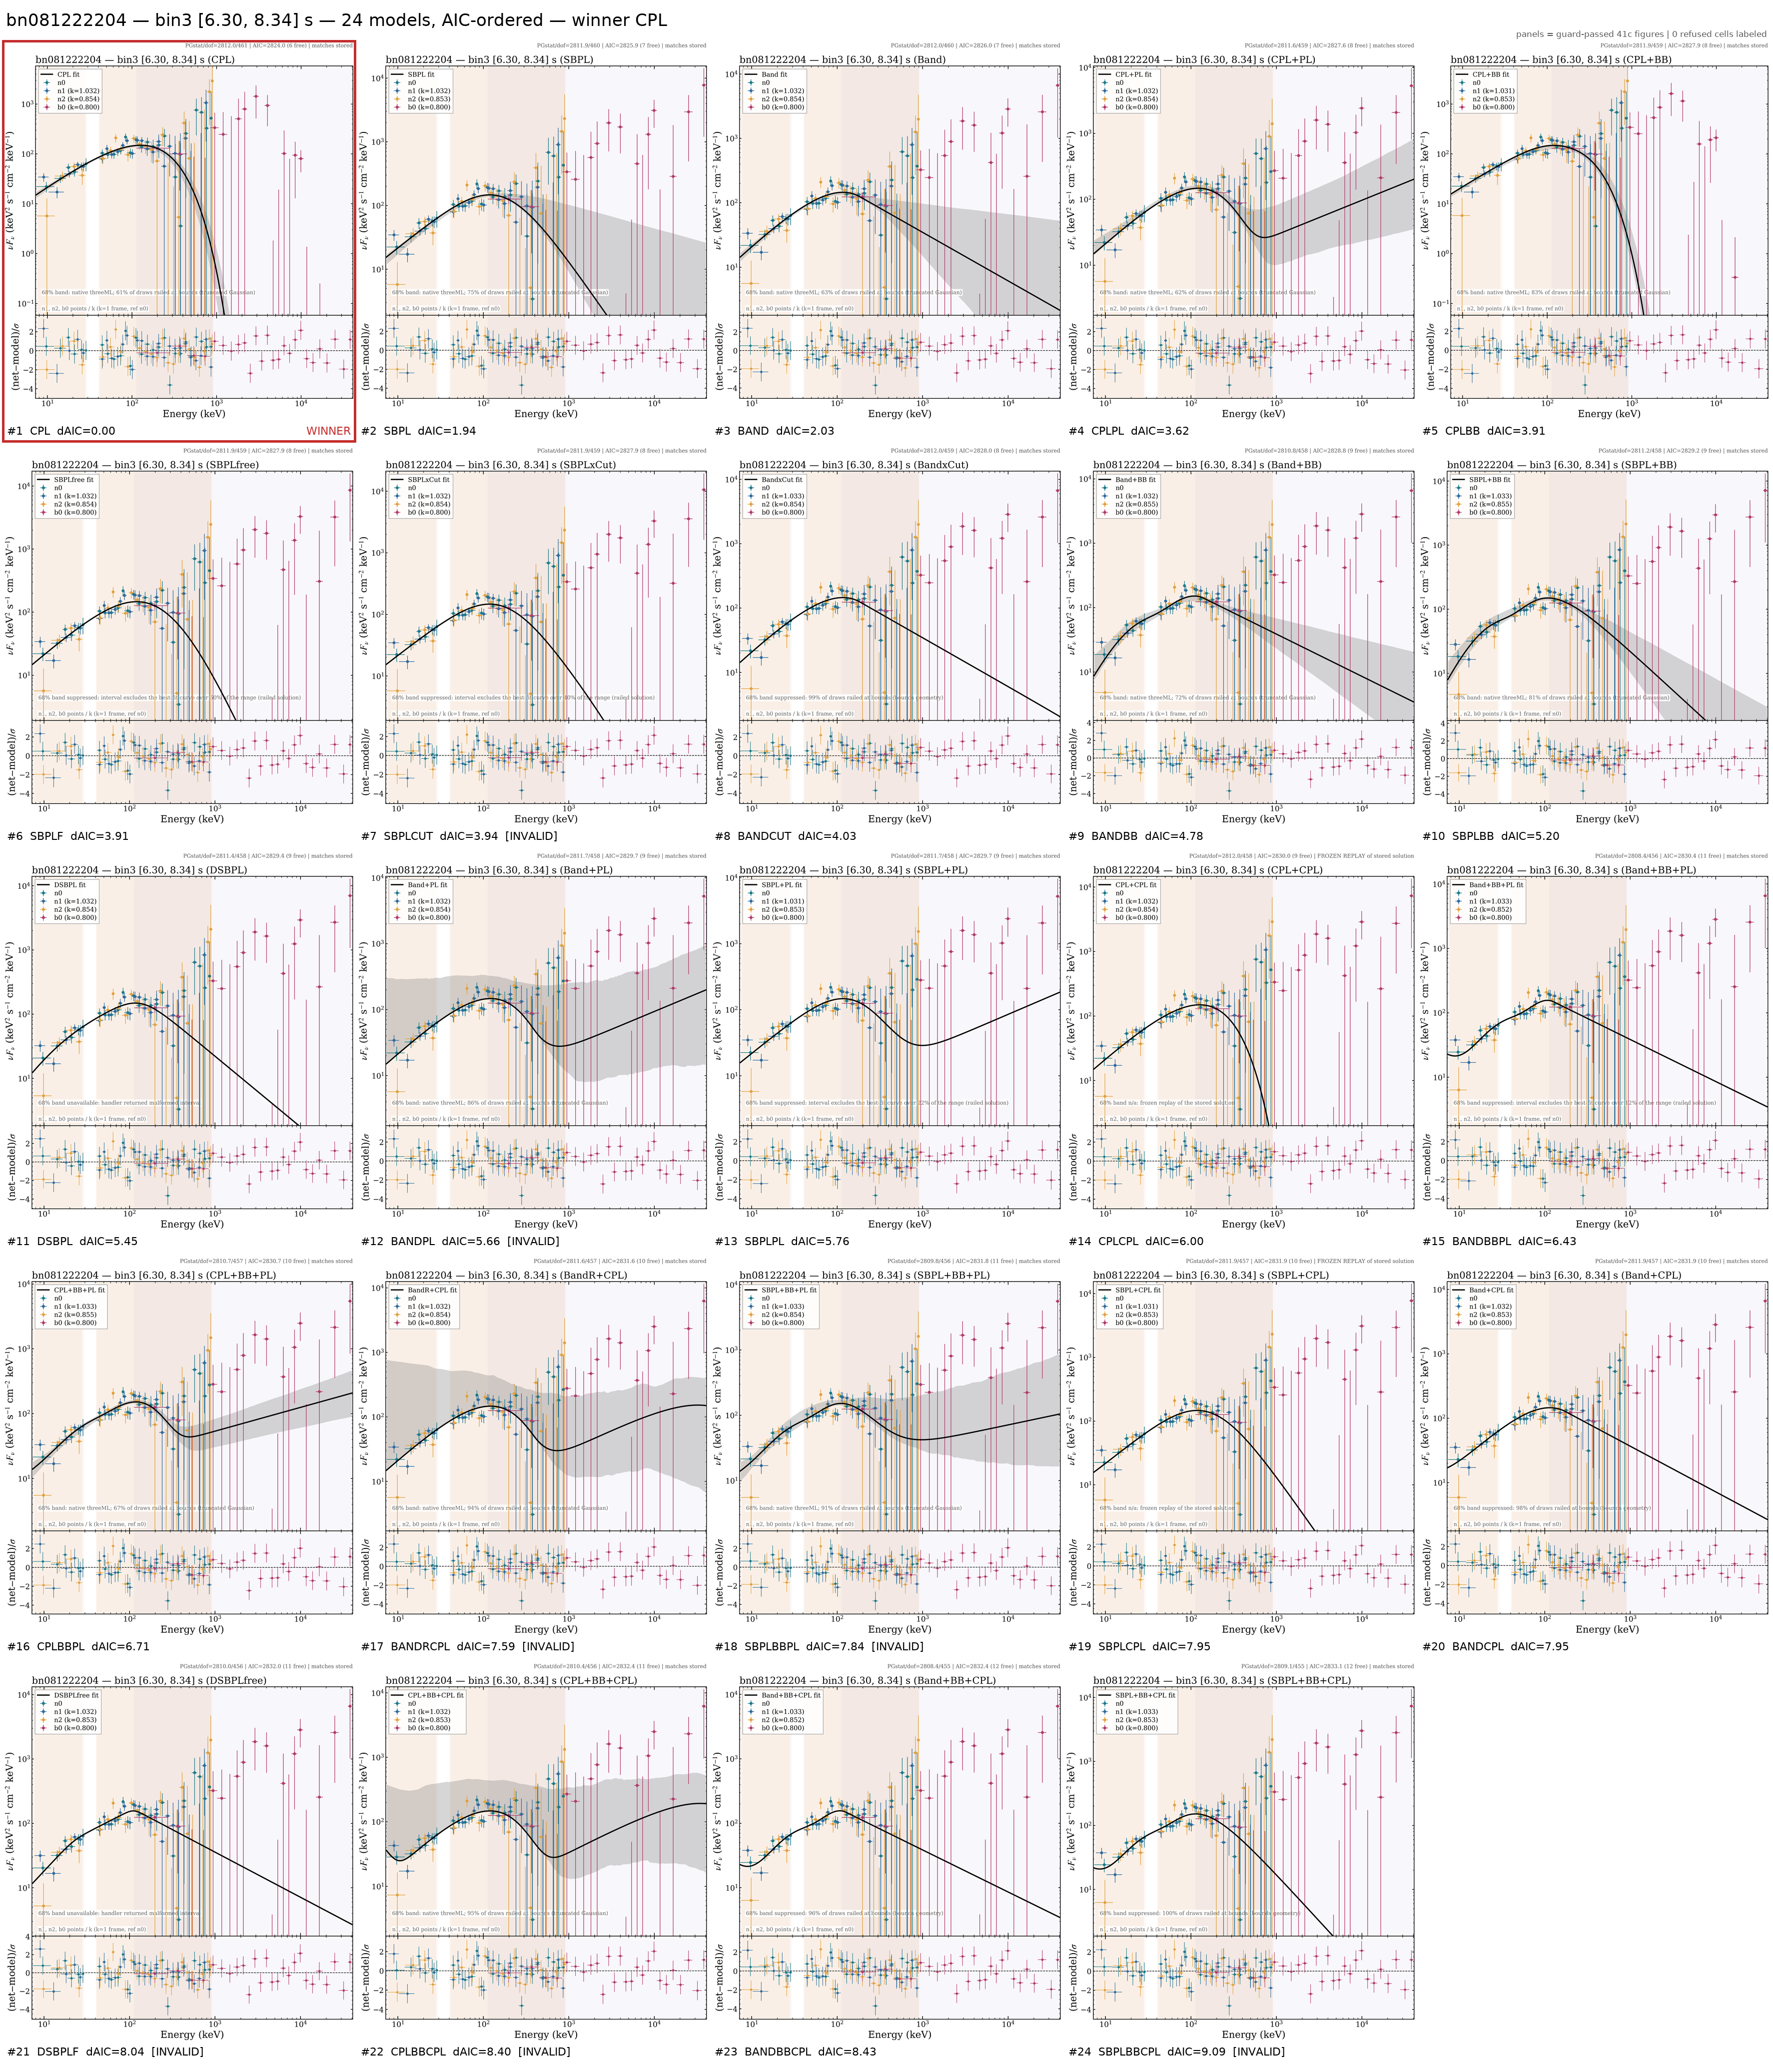
\includegraphics[width=\textwidth]{figs/bn081222204_montage_bin3.png}
\caption{Bin 3 montage.}\end{figure*}
\begin{figure*}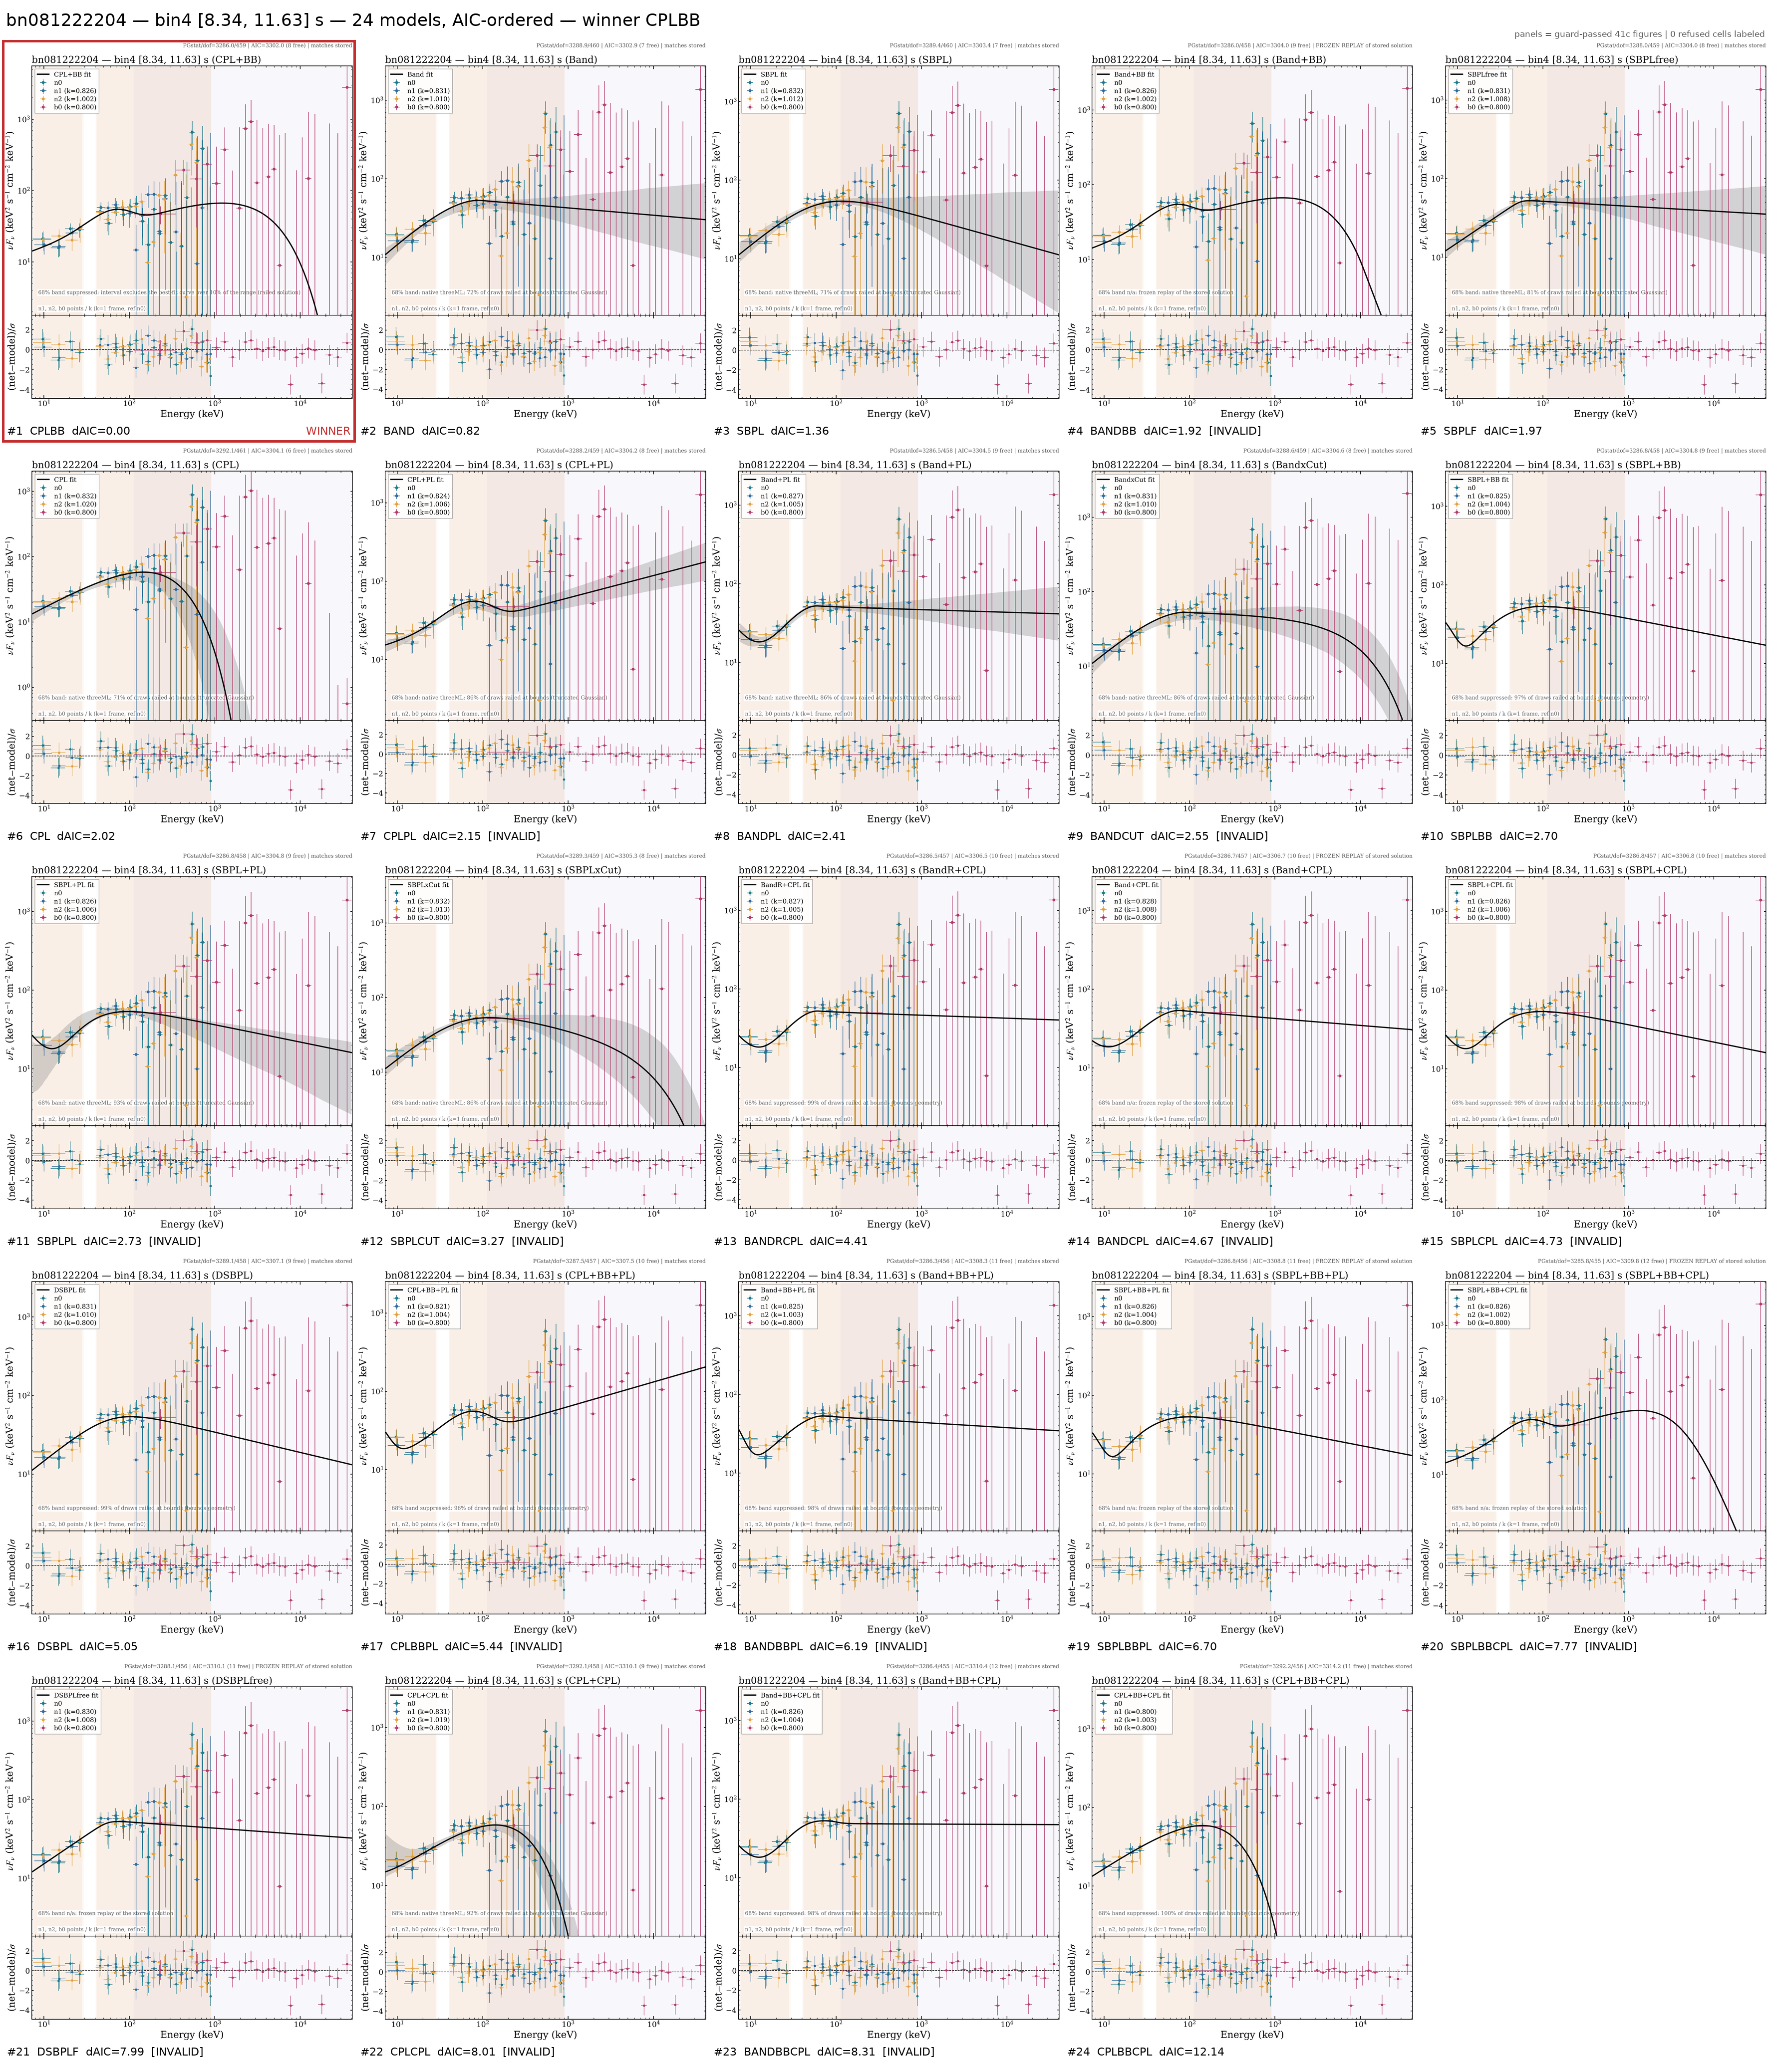
\includegraphics[width=\textwidth]{figs/bn081222204_montage_bin4.png}
\caption{Bin 4 montage.}\end{figure*}
\begin{figure*}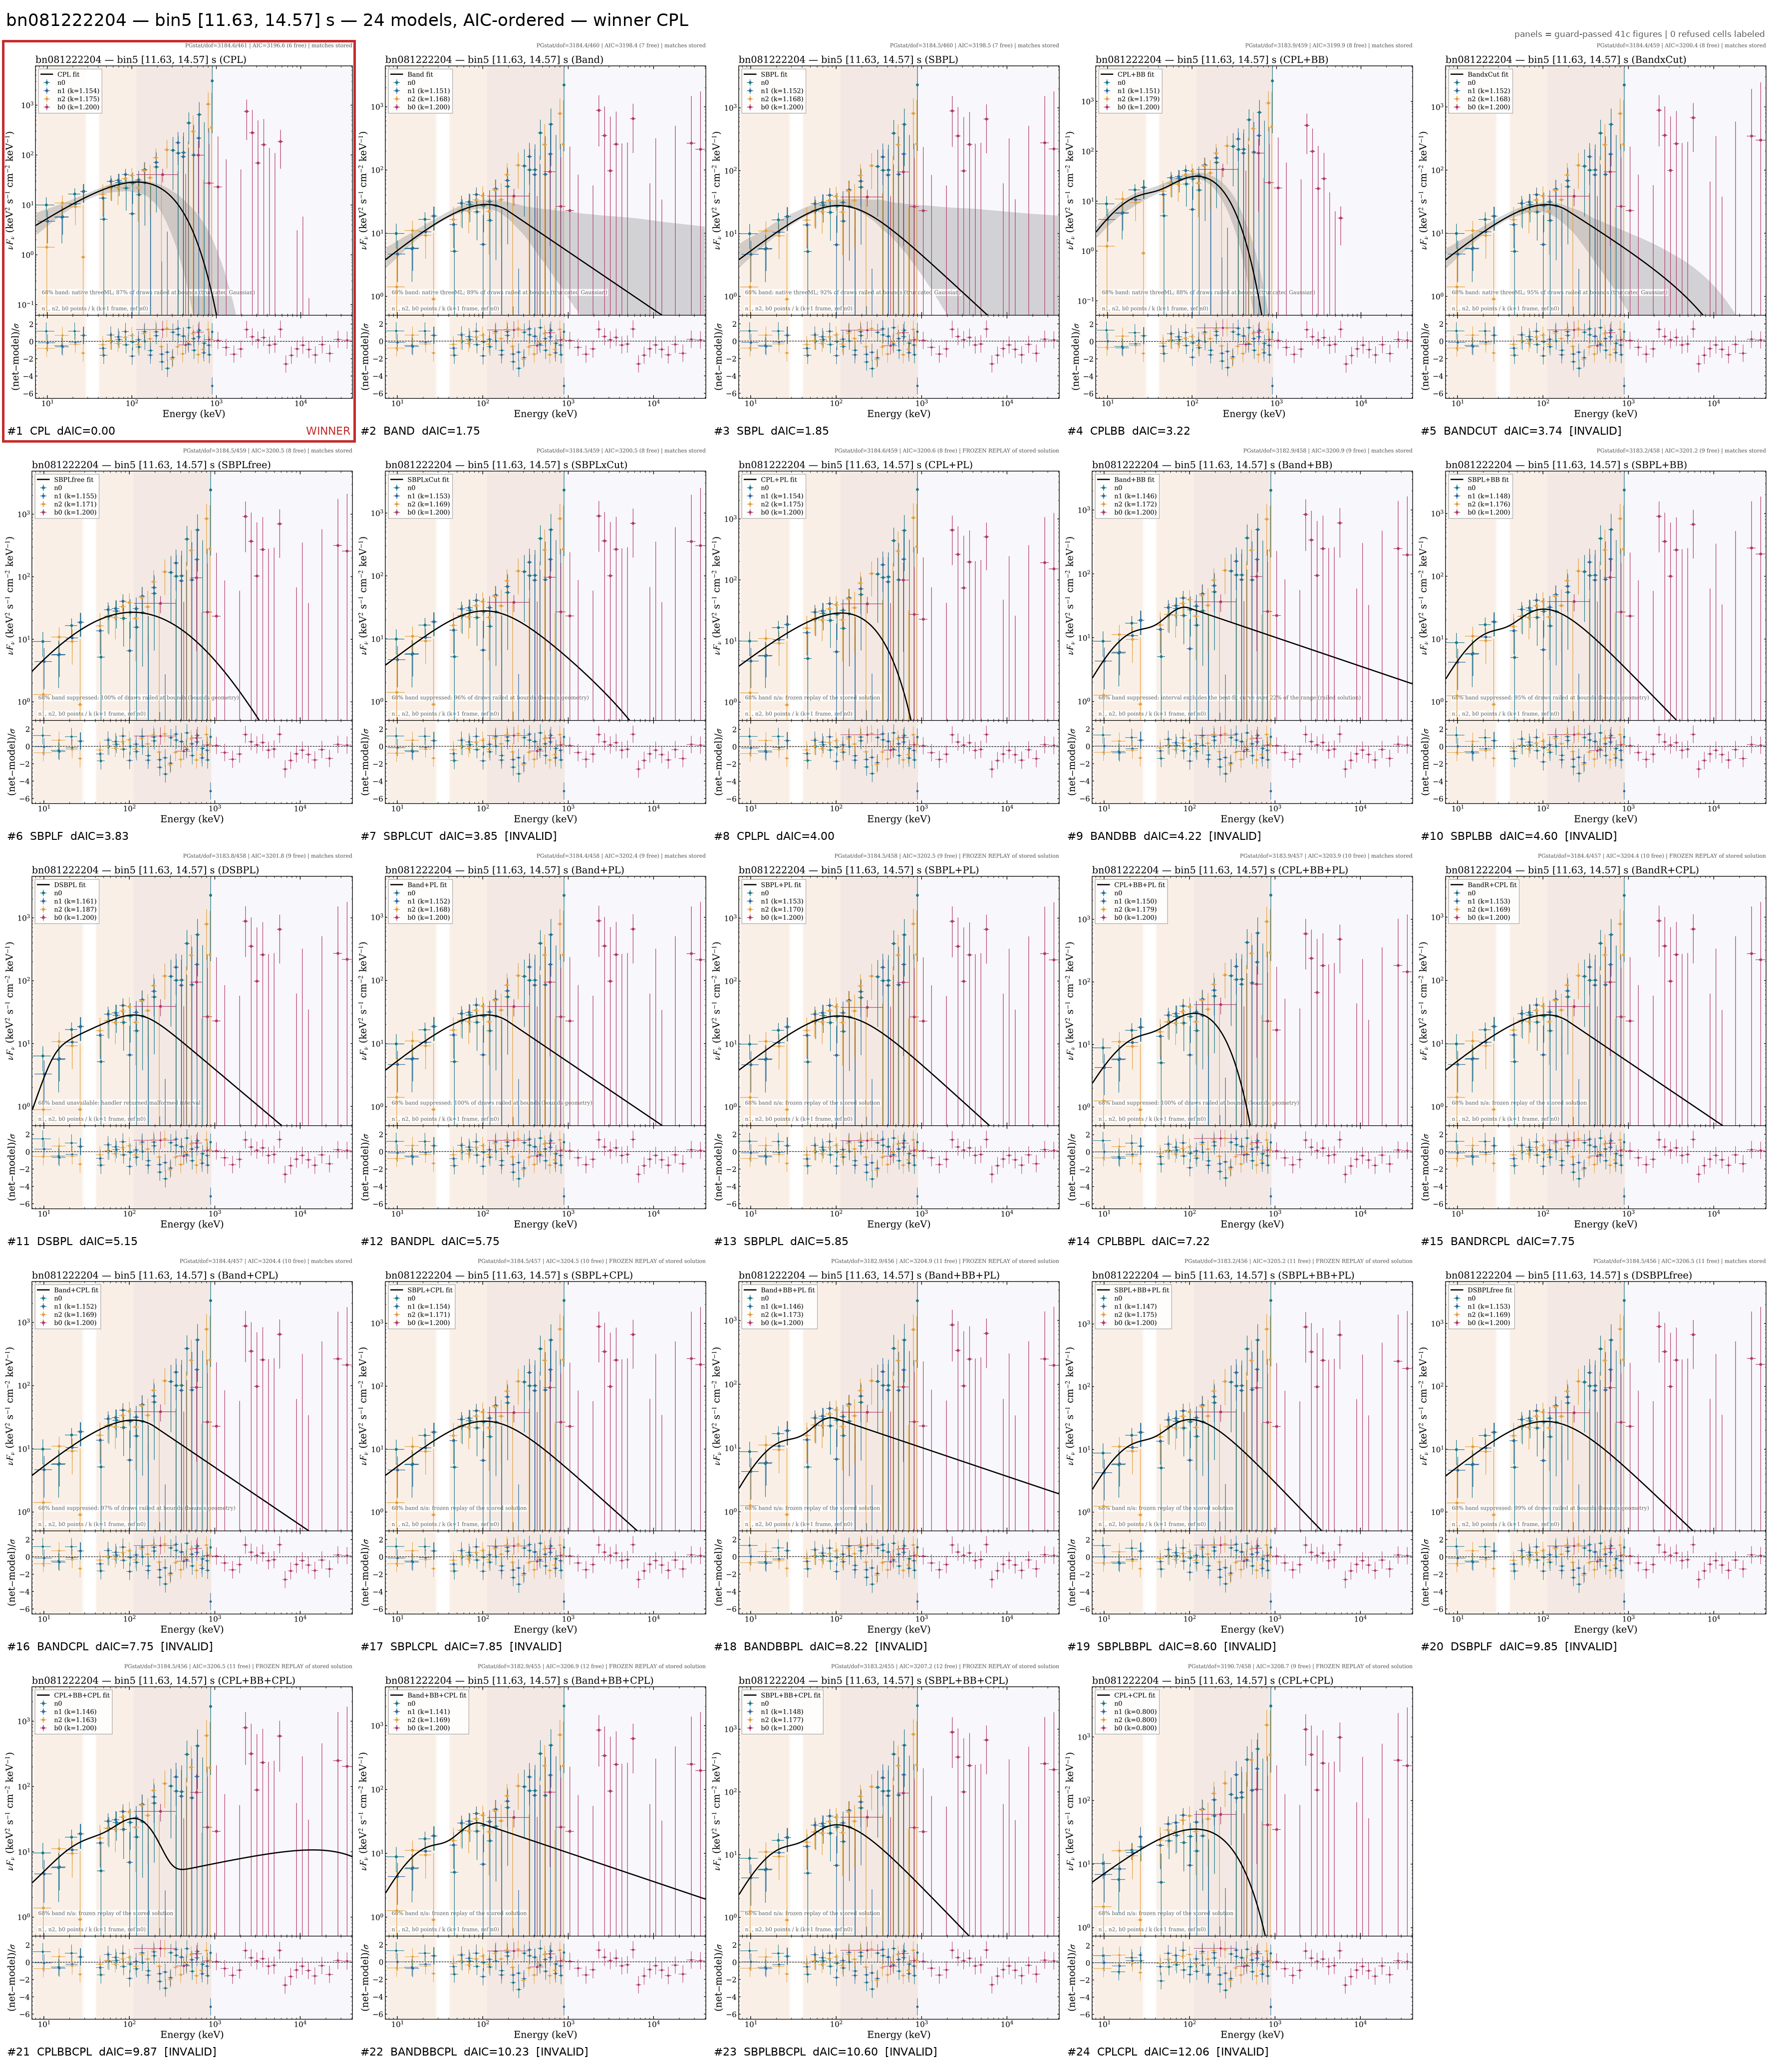
\includegraphics[width=\textwidth]{figs/bn081222204_montage_bin5.png}
\caption{Bin 5 montage.}\end{figure*}

\bibliography{refs}
\bibliographystyle{aasjournal}

\end{document}
